%------ PACKAGES--------
\documentclass[a4paper]{report} % Uses article class in A4 format
\usepackage[utf8]{inputenc}
\usepackage{hyperref}
\usepackage{graphicx}
\usepackage[english]{babel} % Language hyphenation and typographical rules
\usepackage{amsthm, amsmath, amssymb} % Mathematical typesetting
\usepackage{pseudocode} % Environment for specifying algorithms in a natural way
\usepackage{fancyhdr} % Headers and footers
\usepackage{todonotes}
\usepackage{algorithmicx}
\usepackage{algorithm}
\usepackage{algpseudocode}
\usepackage{todonotes}
\usepackage{tikz}
\usepackage{bbold}
\usepackage{footnote}%(Salvo: I added this in order to add footnotes inside algorithms, I hope it does not cause any trouble)
\usepackage{verbatim}%Salvo(For multiline comments)
\usepackage{cancel}%Firas: to strike out terms in an equation
\pagestyle{fancy} 
% All pages have headers and footers
\fancyhead{}\renewcommand{\headrulewidth}{0pt} % Blank out the default header
\fancyfoot[L]{} % Custom footer text
\fancyfoot[C]{} % Custom footer text
\fancyfoot[R]{\thepage} % Custom footer text

\usepackage{subfiles} 
\usepackage{pdfpages}
\usepackage{caption}
\captionsetup{font=scriptsize,labelfont={sf,bf}}
%-------------------


\title{Numerical Methods} 
\author{PCS Students \\ Academic year 2020/2021}
\date{\today} 

\begin{document}
\par

\maketitle
\tableofcontents

\chapter{Statistical Mechanics}
    \section{Introduction}
In molecular dynamics, a thermostat is an algorithm built with the purpose of generating samples from a statistical ensemble at constant temperature $T$.
At this point, we know that the typical choice among the statistical ensembles, when simulating a real physical system, is the Canonical one, which allows fluctuations of the total energy under the constraint that its average remains constant over time.
Therefore, our aim will be to build thermostats which sample configurations drawn from the Canonical ensemble. 

Before entering in the implementation of these algorithms, let's recall some of the main features of the ensemble we are interested in.

\subsection{Recap of the Canonical ensemble}
The probability distribution related to the Canonical ensemble, as defined in Chapter 1 (1.36), is given by
\begin{equation}
     P(x)=\frac{e^{-\beta H(x)}}{Z}
\end{equation}
with 
\begin{equation}
     Z=\int_ {}^{} e^{-\beta H(x)}dx
\label{zetafunc}
\end{equation} 

\par Is important to remember that here $x$ represents a vector that contains the position and momenta of all the particles of the system, so the integral (5.2) is taken over all the points composing the phase space of our system. 

As we have already seen, this formulation allows us to compute the average of a generic observable $A(x)$ as
\begin{equation}
     \langle A \rangle =\int_ {}^{} P(x)A(x)dx,
\end{equation}

and, as a consequence, its variation with respect to the temperature as
\begin{equation}
    \frac{\partial \langle A \rangle}{\partial T}=-\frac{1}{k_B T^2} (-\langle HA \rangle+\langle H \rangle\langle A\rangle). 
\end{equation}

Some relevant examples are the derivatives of the average values of:
\begin{itemize}
    \item The total energy $H$
    \begin{equation}
      \frac{\partial \langle H \rangle}{\partial T}=\frac{1}{k_B T^2} (\langle H^2\rangle-\langle H\rangle^2)=\frac{1}{k_B T^2}\sigma_H^2
    \end{equation} 
    which is proportional to the variance of $H$ (i.e. the amplitude of its fluctuations) and which can be physically interpreted as the amount of energy needed in order for the temperature to increase by 1 degree, i.e. the Heat capacity; 
    \item The potential energy $U$
    \begin{equation}
        \frac{\partial \langle U \rangle}{\partial T}=\frac{1}{k_B T^2} (\langle U^2 \rangle -\langle U \rangle^2)=\frac{1}{k_B T^2}\sigma_U^2 ;
    \end{equation}
    \item the kinetic energy $K$
    \begin{equation}
        \frac{\partial \langle K \rangle}{\partial T}=\frac{1}{k_B T^2} (\langle K^2\rangle-\langle K \rangle^2)=\frac{1}{k_B T^2}\sigma_K^2 .
    \end{equation}
\end{itemize}

In particular, the last two results are obtained exploiting the feature of the Hamiltonian of the majority of the systems we are interested in, built as the sum of a kinetic contribution \begin{math} K(p)=\sum_{i=1}^{N_a} \frac{{p_i}^2}{2m_i} \end{math}, which depends only on the momenta $p_i$ of the particles, and a potential contribution $U(q)$, specific of the system, which depends only on the positions $q_i$. 

This composition of the Hamiltonian makes the probability distribution $P(x=p,q)$ factorizable into two separate parts: \begin{math}P_K(p) \propto e^{-\beta \sum_{i=1}^{N_a} \frac{p_i^2}{2m_i}} \end{math} (which is a gaussian) and $P_U(q)$.

Then, from  $P_K(p)$ we can obtain the probability distribution of the kinetic energies $P_K(K)$, which is not a gaussian (because as $K<0$, $P_K$ is identically equal to $0$), but a Gamma distribution
\begin{equation}
    P_K(K) \propto K^{N_F/2 -1}e^{-\beta K}
\end{equation}
where $N_F=3N_a$ is the number of degrees of freedom, with average
\begin{equation}
    <K>=\frac{3}{2} N_a k_B T \implies \frac{\partial <K>}{\partial T}=\frac{3}{2} N_a k_B
\end{equation}

and width (from (5.7) and (5.8))
\begin{equation}
    \sigma_K=\sqrt{k_B T^2 \frac{\partial <K>}{\partial T}}=\sqrt{\frac{3}{2} N_a k_B^2 T^2}= \sqrt{<K>^2 \frac{2}{3 N_a}}.
\end{equation}
In particular, the factor $K^{N_F/2 -1}$ is in some way related to the density of state: this explains why negative kinetic energies are not allowed ($P_K(K<0)=0$) and why, without the compensation of the Boltzmann factor \begin{math} e^{-\beta K} \end{math}, high kinetic energies would be more likely.
A qualitative description of the behaviour of $P_K(K)$ can be seen in Figure \ref{fig:kinetic distribution}

\begin{figure}
    \centering
    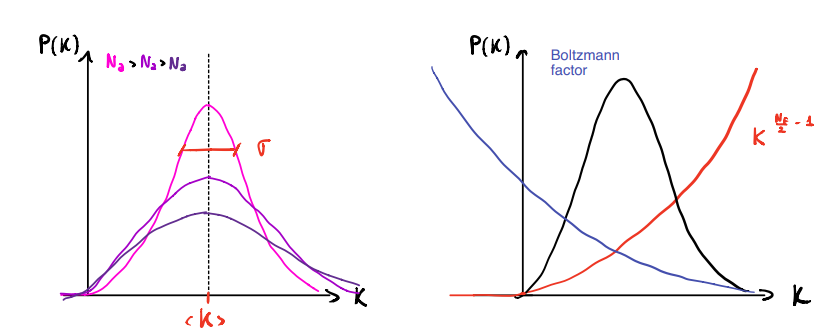
\includegraphics[width=0.7\textwidth]{Thermostats/images/kinetic distribution.PNG}
    \caption{On the left: qualitative behaviour of the Gamma distribution $P_K(K)$ at different values of $N_a$, always centered in the same value in order to compare visually the different shapes. On the right: qualitative behaviour of the two factors that compose $P_K(K)$, whose coexistence leads to the typical shape of the Gamma distribution.}
    \label{fig:kinetic distribution}
\end{figure}

\section{Algorithms}

As mentioned in the Introduction, the two main properties of the thermostats we want to implement are:
\begin{itemize}
    \item Equilibration of the system to a target value of the temperature $\bar T$, that, after an early transient, have to remain constant;
    \item Production of configurations drawn from the Canonical ensemble.
\end{itemize}

First of all, we have seen, as one of the main results of the theoretical description of the Canonical ensemble, that \begin{math} <K> \propto T \end{math}. 
Therefore, we can think about controlling the value of the temperature through the control of the kinetic energy $K(p)$, which will have to reach the target value $\bar K \propto \bar T$. This control on $K(p)$ can be realized imposing proper variations of $K(p)$ itself, in such a way that $<K>= \bar K$. 

But this will not be sufficient in order to satisfy the second request: in fact, in order for our simulation to produce canonical configurations, we need also the fluctuations on $K(p)$ to be coherent with the canonical distribution, and so equal to its variance $\sigma_K^2$.

As a consequence of these requirements, the main idea to implement thermostats is by choosing a rule for the variation of $K(p)$, and evolving the system through a modified version of Hamilton equations, which will determine variations of potential energy $U(q)$ in such a way that the ones of $K(p)$ are balanced, and so that the total energy is approximately conserved.


\subsection{Trial and error}

The first attempt, which can not be called an actual algorithm, but is useful to introduce us to the logic underlying thermostats, is the "Trial and error". 
It exploits the behaviour of the simulation to set the proper value of the initialization $K_0$ which, after a transient, will lead to the target value \begin{math} \bar K \end{math} (and so to the target value \begin{math} \bar T \end{math}).

At first, in fact, we could try initializating the kinetic energy at its target value. Unfortunately, starting the simulation we would see that $K$ doesn't remain constant at $\bar K$, but equilibrates to a different value.

So, we could think of starting a new simulation from a different $K_0$, shifted from the previous by the difference between $\bar K$ and the previous equilibration value.
Typically, the optimal result can not be reached in a unique attempt, but after various iterations, which can be stopped when the difference between $\bar K$ and the new equilibration value of $K$ is small enough.

\begin{figure}
    \centering
    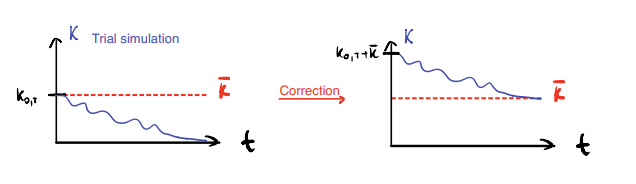
\includegraphics[width=0.7\textwidth]{Thermostats/images/Trial and error.PNG}
    \caption{The first image represent the Trial simulation, where the kinetic energy is initialized to its target value. The second represent the correct simulation, where the initialization is set to that value from which, after the equilibration, the kinetic energy reaches the target value.}
    \label{fig:trial and error}
\end{figure}

In Figure \ref{fig:trial and error} we see how this procedure would look if a unique attempt would be sufficient.

Unfortunately, as we can imagine looking at the triviality of this algorithm, this is not a suitable choice for implementing a thermostat.

\subsection{Velocity rescaling}
The Velocity rescaling algorithm is based on the following idea:
\begin{itemize}
    \item Given an initial configuration of the system, we run a number \textit {stride} of steps using a Hamilton equations integrator, like, for example, Velocity Verlet;
    \item We check the istantaneous value of $K$ and we change it rescaling it by a factor that makes it equal to the target value $\bar K=\frac{3}{2}N_a K_B \bar T$.
\end{itemize}

A pseudocode representing these operations would be:
\begin{algorithm}[H]\label{velocity_rescaling}
			\caption{Velocity rescaling algorithm}
			\begin{algorithmic}[1]
				\For{$i step\; inrange (nsteps)$}
    				\State $p+=f*\Delta t/2$
    				\State $q+=p*\Delta t/m$
    				\State $p+=f*\Delta t/2$
    				\If{$i step\%stride==0$}
    				    \State $K= \frac{\sum_{i}{p_i^2}}{{2m_i}}$
    				    \State $p* = \sqrt{\frac{\Bar{K}}{K}}$
    				\EndIf
				\EndFor
			\end{algorithmic}
		\end{algorithm}

\begin{figure}
    \centering
    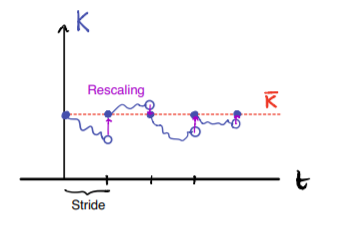
\includegraphics[width=0.7\textwidth]{Thermostats/images/velocity rescaling.PNG}
    \caption{Example of a trajectory $K(t)$ produced using the Velocity rescaling thermostat.}
    \label{fig:velocity rescaling}
\end{figure}		

As we can see, in this case the change in the kinetic energy is made on its total value, and not on the specific values $K_i$ of the single particles: this feature defines the so called \textit {Global thermostats}.

Although, as also qualitatively represented in Figure \ref{fig:velocity rescaling}, this algorithm works well in the equilibration to the target value $\bar K$, reached in a time interval $\propto {\textit {stride}}$, this is not an optimal choice for two main reasons: first of all, the distribution we are sampling from is unknown, and certainly it is not the canonical since the fluctuations of $K$ are not the proper ones (see Figure \ref{fig:fluctuations}); then, the trajectory is discontinuous, and this does not allow us to convert the algorithm into a differential equation.

\begin{figure}
    \centering
    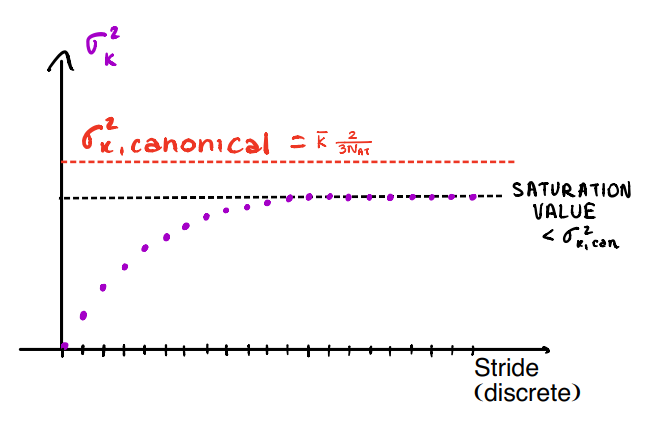
\includegraphics[width=0.7\textwidth]{Thermostats/images/fluctuations.PNG}
    \caption{Behaviour of $\sigma_K^2$ as a function of \textit {stride}. If \textit {stride} is small, the trajectory is smoother and $<K>=\bar K$, but the fluctuations are too small. If \textit{stride} is too big, the fluctuations will reach a saturation value smaller than the correct one, and also $K$ doesn't reach the target: in fact, this choice would basically correspond to evolving the system according to Velocity Verlet, which guarantees the conservation of the total energy and then produces configurations drawn from the Microcanonical distribution. }
    \label{fig:fluctuations}
\end{figure}

\subsection{Berendsen thermostat}
The problem of discontinuity in Velocity rescaling algorithm is soon solved by the Berendsen thermostat, which can be interpreted as its "continuous version".

It is based on the idea of modifying $K$ at each step, rescaling it by a properly weighted sum of the current value and the target value.

In practice, this operation would consist into the multiplication of the current value of the momentum $p$ by a factor
\begin{equation}
    F={\sqrt{\frac{c_1K+c_2 \bar K}{K}}}.
\end{equation}

In particular, the choice of the weights ${c_1}$ and ${c_2}$ has to guarantee the following properties:
\begin{itemize}
    \item $c_1+c_2=1$
    since, when $K=\bar K$, the factor F must be equal to 1, because the target value has been reached, and then we do not have to modify the current value;
    \item the limit $c_1 \rightarrow 1$ ( $\implies c_2 \rightarrow 0$), which represents the absence of the thermostat (since there are no corrections to the current values $p$) should coincide with the limit case of $\textit{stride}=\tau \rightarrow \infty$ in Velocity rescaling;
    \item the limit $c_2 \rightarrow 1$ ($\implies c_1 \rightarrow 0$), which basically respresents the application of Velocity rescaling at each step, should coincide with the limit case of $\textit{stride}=\tau \rightarrow 0$.
\end{itemize}

A choice which guarantees the latter requests is:
\begin{equation}
   c_1=e^{-{\frac{\Delta t}{\tau}}} ;\quad
      c_2=1-c_1=1-e^{-{\frac{\Delta t}{\tau}}}
\end{equation}

At this point, we can try converting the algorithm into a differential equation:
\begin{multline*}
    K_{new}={\frac{e^{-{\frac{\Delta t}{\tau}}}K+\left(1-e^{-{\frac{\Delta t}{\tau}}}\right) \bar K}{K}}K \\ 
    \implies \Delta K=K_{new}-K=e^{-{\frac{\Delta t}{\tau}}}K + (1-e^{-{\frac{\Delta t}{\tau}}}) \bar K - K \\
    = (1-e^{-{\frac{\Delta t}{\tau}}} )(\bar K -K) 
\end{multline*}

Then, performing the infinitesimal limit:
\begin{equation*}
    \lim_{{\Delta t}\to 0} \Delta K = (1-1+\frac{\Delta t}{\tau} + \textit{h.o.t})(\bar K-K)=\frac{\Delta t}{\tau}(\bar K-K)
\end{equation*}

\begin{equation}
    \implies dK=dt \frac{(\bar K-K)}{\tau}
\end{equation}

that is actually a differential equation. This means its solution, i.e. $K(t)$, is continuous, and then we can say that the issue we had with Velocity rescaling is solved.

Another advantage with respect to Velocity rescaling is that now we have a control parameter $\tau$, which, differently from \textit{stride}, has a physical interpretation:
it is the relaxation time of the system, and gives a qualitative measure of the thermal inertia of it, since the greater is $\tau$, the more difficult will be to change $K$, namely $T$.

Moreover, as a smoother version of Velocity rescaling, Berendsen's is itself a global thermostat.

So, in conclusion, one of the main advantages of using this algorithm is that the trajectories it produces are continuous, but it is not the only one. In fact, according to the huge number of citations of the original paper by Berendsen (1984), it is probably the most used thermostat, and this is due to a series of properties: it empirically equilibrates well; it is easy to understand; it is efficient. Regarding the efficiency, this is what actually makes people prefer this algorithm to more exact ones like, for example, Hybrid Montecarlo: indeed, the approximation makes Berendsen thermostat quicker in simulating very large systems, for  which a more accurate algorithm would take a too long time.

However, this algorithm does not sample configurations from the canonical distribution. In fact, even if balance is satisfied, because a stationary distribution can be reached, this is not the canonical one, and this is due to the fact that $K$ does not respect the proper fluctuations. Detailed balance is instead not guaranteed, because $K$ is forced to reach $\bar K$ and a time-reversed trajectory is not even possible.




    \section{Maximum entropy principle and microcanonical ensemble}
As before, consider a system divided in two compartments with energies $E_1$ and $E_2$. The two subsystems can exchange energy, but the sum $E_1+E_2 = E$ is fixed. We have already demonstrated that the phase space of the system at the equilibrium is given by 
\begin{equation}
    \Gamma_{1+2}(E) = \Gamma_1(E_1^*)\,\Gamma_2(E-E_1^*),
\end{equation}
where $E_1^*$ is the energy that maximizes $\Gamma_{1+2}$. This relation is clearer if one thinks of $\Gamma_i$ as the degeneracy of a state with an energy $E_i$. The equilibrium condition then becomes
\begin{equation}
    \frac{\partial \Gamma_{1+2}}{\partial E_1}\bigg|_{E_1^*} = \frac{\partial \Gamma_1(E_1)}{\partial E_1} \Gamma_2(E - E_1) + \Gamma_1(E_1)\frac{\partial \Gamma_2(E - E_1)}{\partial E_1} = 0.
\end{equation}
Since we have the constraint $E_2 = E-E_1$, we can take the derivative of $\Gamma_2$ with respect to $E_2$, changing its sign. Ordering the terms and multiplying by the Boltzmann constant $k_B$ we obtain
\begin{equation}
    \frac{k_B}{\Gamma_1} \frac{\partial \Gamma_1}{\partial E_1} = \frac{k_B}{\Gamma_2} \frac{\partial \Gamma_2}{\partial E_2} \: \Longrightarrow \:
    k_B \frac{\partial (\ln{\Gamma_1})}{\partial E_1} = k_B \frac{\partial (\ln{\Gamma_2})}{\partial E_2}
\end{equation}
and $k_B\ln{\Gamma}$ was our definition of entropy $S$. So the equilibrium condition is 
\begin{equation}
    \frac{\partial S_1}{\partial E_1} = \frac{\partial S_2}{\partial E_2}
\end{equation}
which is equivalent to having the same temperature. \\ \\

Entropy is an observable, so its expected value can be written as $S = \int d\Gamma \rho f(q,p)$ for a certain function $f$ of positions and momenta. From an analogy with probability theory and Shannon entropy, entropy turns out to be
\begin{equation}
    S = -\int d\Gamma \rho \ln{\rho}.
\end{equation}
which is also equal to $S=\ln{\Gamma}$ (for $k_B=1$).
We don't give a formal proof of this statement, but we show that it gives correct results in two particular limit cases:
\begin{itemize}
    \item case 1: $n$ energy levels, with $p_1 = 1$ and $p_{i\neq 1} = 0 \: \Rightarrow \: S=0$. \\
    \item case 2: $p_i = 1/n$ for all $i \: \Rightarrow \: S= -\frac{1}{n}\ln(\frac{1}{n})^n = \ln{n}$.
\end{itemize}
The maximum entropy principle states that a system in equilibrium tends to maximize entropy, given the constraints, for every probability density $\rho$. For the microcanonical ensemble, we consider the following constraints for $\rho$:
\begin{gather}
    \int d\Gamma \rho = 1 \: \Rightarrow \: \text{normalization} \\
    \rho(\mathbf{q},\mathbf{p}) = 0 \: \text{if} \: H(\mathbf{q},\mathbf{p}) \not\in (E,E+\Delta).
\end{gather}
For $k_B=1$, $S = -\int d\Gamma \rho \ln{\rho}$ and introducing the Lagrange multiplier $\lambda$ we can construct the functional
\begin{equation}
    \mathcal{F}[\rho] = -\int d\Gamma (\rho \ln{\rho} - \lambda\rho)
\end{equation}
and our goal is to find $\rho^*$ that makes it stationary. More explicitly, we want the functional differential
\begin{equation}
    \partial\mathcal{F}[\rho^*] \equiv \mathcal{F}[\rho^*+\delta\rho] - \mathcal{F}[\rho^*]
\end{equation}
with no linear terms in $\delta\rho$. Then we get
\begin{align}
\label{eq:rho_micro}
    \partial\mathcal{F}[\rho^*] &= -\int d\Gamma [(\rho^*+\delta\rho)\ln(\rho^*+\delta\rho) - \lambda(\rho^*+\delta\rho)] + \int d\Gamma (\rho^*\ln\rho^* - \lambda\rho^*) \nonumber \\
    &= -\int d\Gamma (\delta\rho\ln{\rho^*}+\delta\rho-\lambda\,\delta\rho) + h.o.t. \nonumber \\
    &= -\int d\Gamma \delta\rho \,(\ln{\rho^*}+1-\lambda) = 0
\end{align}
where in the second line we have used the fact that 
\begin{equation}
    \ln(\rho^*+\delta\rho) \simeq \ln{\rho^*} + \frac{\delta\rho}{\rho^*} + h.o.t.
\end{equation}
Since eq. (\ref{eq:rho_micro}) has to hold for every $\delta\rho$, the integrand must be null, i.e.
\begin{equation}
    \ln{\rho^*}(\mathbf{q},\mathbf{p}) = \lambda-1
\end{equation}
that does not depend on $\mathbf{q}$ and $\mathbf{p}$, so we obtain a uniform \textit{a priori} probability. This is due to the fact that we had no constraints, except for the normalization of the probability density. We can repeat the same calculation adding the constraint 
\begin{equation}
    \int d\Gamma \rho\,H = \bar{E}
\end{equation}
that corresponds to the canonical ensemble.




    %by Elena C. WORK IN PROGRESS
\subsection{Leapfrog Algorithm}
The Velocity Verlet algorithm shown previously (Algorithm \ref{alg:velocity_verlet}) can be modified to reduce the computational cost.\\ In particular, compute a force is quite expensive: computing the force twice will require twice the simulation time. One solution to reduce the computational cost is to merge the momenta shifts together (using the same value of the force): this leads to a slightly faster simulation, but on the other side this kills the possibility of printing the values of p and q at the same time (access to the phase space). This solution is called \textbf{Leapfrog algorithm}.\\
\begin{algorithm}[H]
			\caption{Leapfrog algorithm}
			\label{alg:leapfrog}
			\begin{algorithmic}[1]
			    \State $p=p+f*\Delta t/2$	\For{$i=1,...,nsteps$}
    			\State	$q=q+p/m \Delta t$
                 \State	$f=force(q)$
    			\State	$p=p+f*\Delta t$
				\EndFor
			\end{algorithmic}
		\end{algorithm}
Momentum and position are moved in an alternate way: at the end of a cycle, we do not find the values of the positions and momenta at the same timestep, they are found at a difference of half timestep. Slightly faster than Velocity Verlet, not very significant. 
\begin{figure}[H]
    \centering
    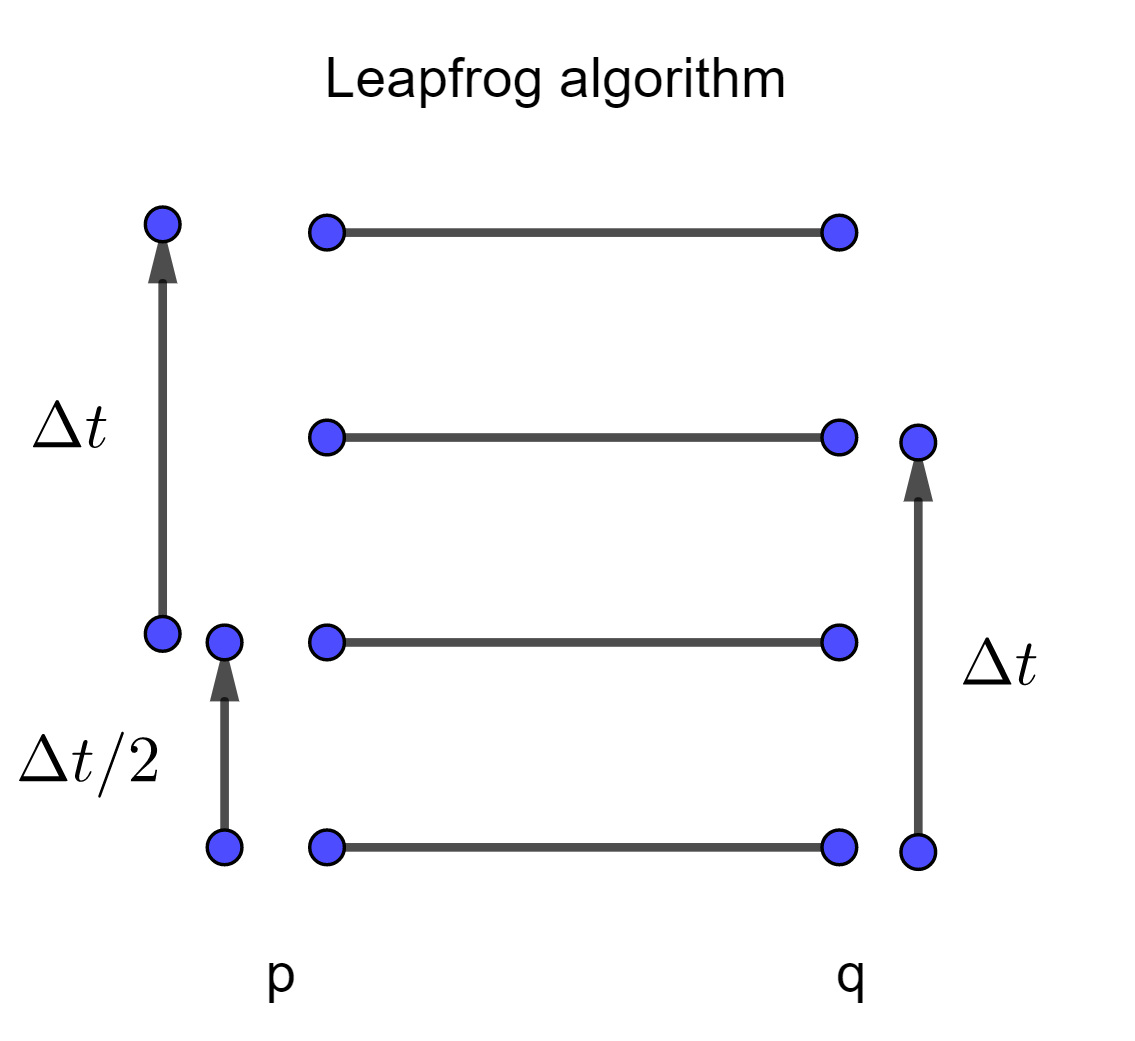
\includegraphics[width=50mm,scale=0.5]{Integrators/images/leapfrog.png}
    \caption{Scheme of the leapfrog algorithm}
    \label{fig:leapfrog}
\end{figure}
\subsection{Position Verlet}
Another alternative to the Velocity Verlet algorithm it is the so-called \textbf{Position Verlet algorithm}.
\begin{algorithm}[H]
			\caption{Position Verlet}
			\label{alg:position_verlet}
			\begin{algorithmic}[1]
        	\For{$i=1,...,nsteps$}
			\State	$q=q+p/m* \Delta t/2$
			\State	$f=force(q)$
			\State	$p=p+f*\Delta t$
			\State	$q=q+p/m* \Delta t/2$
				\EndFor
			\end{algorithmic}
		\end{algorithm}
This algorithm is the swapped version of Velocity Verlet, where the free particle is evolved for half timestep, then the infinite mass system is evolved for one timestep, then the free particle again for half timestep. 
\begin{itemize}
    \item \textbf{Advantages:} the force is computed only once, which is computationally advantageous (only one update of the momentum).
    \item \textbf{Disadvantages:} I cannot print the total energy. Potential energy needs to be computed with a similar procedure to the computation of forces (very expensive). Therefore, it is more convenient to compute forces and energies at the same time, but it is not possible with Position Verlet. Moreover, this algorithm is less used than Velocity Verlet, which is the simplest one.
\end{itemize}

\subsection{Other considerations on the Velocity Verlet algorithm}
Let us recall the Velocity Verlet algorithm:
    \begin{equation}\label{velocityverlet}
            \begin{cases}
                q(t+\Delta t)= q(t)+\frac{p(t)}{m}\Delta t+ \frac{f(t)}{m}\frac{\Delta t^2}{2}\\
                p(t+\Delta t)= p(t)+\frac{f(t)}{2}\Delta t+ \frac{f(t+\Delta t)}{2}\Delta t
            \end{cases}
            \end{equation}
Let's prove that the trajectories obtained with Velocity Verlet are equivalent to those obtained with Verlet algorithm. Trajectories are exactly time reversible, which means that we are allowed to compute $q(t-\Delta t)$ changing the sign of $\Delta t$ in the first equation \ref{velocityverlet}:
\begin{equation}\label{t-dt}
q(t-\Delta t)= q(t)-\frac{p(t)}{m}\Delta t+ \frac{f(t)}{m}\frac{\Delta t^2}{2}
\end{equation}
Let us sum $q(t-\Delta t)$ and $q(t+\Delta t)$ (first eq. \ref{velocityverlet} and eq. \ref{t-dt}):
\begin{equation*}
    q(t-\Delta t)+q(t+\Delta t)=2q(t)+\frac{f(t)}{m}\Delta t^2
\end{equation*}
This is consistent because equation \ref{velocityverlet} for the positions resembles a Taylor expansion of q.  The introduction of operator formalism is significant only for the sake of studying the evolution of momenta, while the evolution of positions is equivalent to the one obtained with the Verlet algorithm. 
In fact, the same trajectory results from the application of Verlet and Velocity Verlet algorithms.\\
Differences between the two algorithms are found by the fact that the Verlet algorithm considers differences between positions (current position $q(t_0)$ minus previous position $q(t_0-\Delta t$)): this leads to large round-off errors. Meanwhile, this problem is not present in Velocity Verlet, which is more numerically stable. Moreover, Velocity Verlet already includes a definition of the velocity, not present in Verlet algorithm: in the former case it is possible to compute the total energy and check if it is conserved.
We recall the properties of Velocity Verlet already discussed in section \ref{chapt:properites_vel_verlet}:
\begin{itemize}
\item \textbf{Trajectory is time reversible.}
\item \textbf{Volume in phase space is conserved.}
\item \textbf{Energy is not conserved}
\end{itemize}
Let us check the latter property for a simple example.
\subsubsection{Harmonic oscillator}
Force is given by 
\begin{equation*}
    f=- k q
\end{equation*}
Change slightly the notation:
\begin{equation*}
    \begin{cases}
        q=q(t)\\
        q'=q(t+\Delta t)
    \end{cases}
\end{equation*}
\begin{equation*}
    \begin{cases}
        q'=q+\frac{p}{m}\Delta t -\frac{k}{m}\frac{q \Delta t^2}{2}=(1-\frac{k}{m}\frac{\Delta t^2}{2})q+\frac{\Delta t}{m}p\\
        p'=p-\frac{k q \Delta t}{2}-\frac{k q' \Delta t}{2}
    \end{cases}
\end{equation*}
Substituting the first equation into the second equation we obtain:
\begin{equation}
    p'=p-k q \Delta t-\frac{k p \Delta t^2}{2m}+\frac{k \Delta t^3 k q}{4 m} = (1-\frac{k}{2m}\Delta t^2)p+(-k \Delta t+\frac{k^2 \Delta t^3}{4 m})q
\end{equation}
In a matrix form:\\
\begin{equation}
  \begin{pmatrix}
    q'\\
    p'
  \end{pmatrix}
  =
  \begin{pmatrix}
    1-\frac{k}{m}\frac{\Delta t^2}{2} & \frac{\Delta t}{m} \\
    -k \Delta t+\frac{k^2 \Delta t^3}{4 m} & 1-\frac{k}{m}\frac{\Delta t^2}{2}
  \end{pmatrix} 
  \begin{pmatrix}
    q \\
    p
  \end{pmatrix}
\end{equation}
  If k=m=1 (unit-less expression):
\begin{equation}
  \begin{pmatrix}
    q'\\
    p'
  \end{pmatrix}
  =
  \begin{pmatrix}
    1-\frac{\Delta t^2}{2} & \Delta t \\
    -\Delta t+\frac{\Delta t^3}{4} & 1-\frac{\Delta t^2}{2}
  \end{pmatrix} 
  \begin{pmatrix}
    q \\
    p
  \end{pmatrix}
\end{equation}
If energy is conserved, the exact solution should be given by a circular trajectory. In other words, the energy conservation is satisfied if the transformation matrix is a rotation.
A rotation matrix is given by
\begin{equation}
A=
    \begin{pmatrix}
      \cos{\theta} & -\sin{\theta} \\
      \sin{\theta} & \cos{\theta}
    \end{pmatrix}
\end{equation}
Therefore, we could impose $\cos{\theta}=1-\frac{\Delta t^2}{2}$ and it is okay because the elements on the diagonal are equal, but $ \Delta t\neq -(-\Delta t+\frac{\Delta t^3}{4})$ in general. Let us also check if the determinant is equal to 1 as the determinant of a rotational matrix.
\begin{equation}
    det(A)= \left(1-\frac{\Delta t^2}{2}\right)^2-\left(-\Delta t+\frac{\Delta t^3}{4}\right)*\Delta t =1
\end{equation}
Still, this is not exactly a rotational matrix but only approximately. This implies that, starting from a point on the trajectory, the next one will not follow the exact trajectory. In order to study the behaviour of the trajectory, i.e., if the trajectory explodes, implodes or fluctuates, let us consider the eigenvalues of $A$.
\begin{equation}
det(A-\lambda \mathbb{1})=(1-\frac{\Delta t^2}{2}-\lambda)^2-(-\Delta t+\frac{\Delta t^3}{4})*\Delta t=0
\end{equation}
\begin{equation*}
(1-\frac{\Delta t^2}{2}-\lambda)^2=(-\Delta t+\frac{\Delta t^3}{4})*\Delta t
\end{equation*}
\begin{equation*}
    \lambda_{1,2}=1-\frac{\Delta t^2}{2}\pm \sqrt{-\Delta t^2 + \frac{\Delta t^4}{4}} 
\end{equation*}
Eigenvalues can be either both real or both complex and conjugated (see graph \ref{fig:complexplane}) in the former case, their product should be 1 ($\lambda_1*\lambda_2=1$). 
\begin{figure}[H]
    \centering
    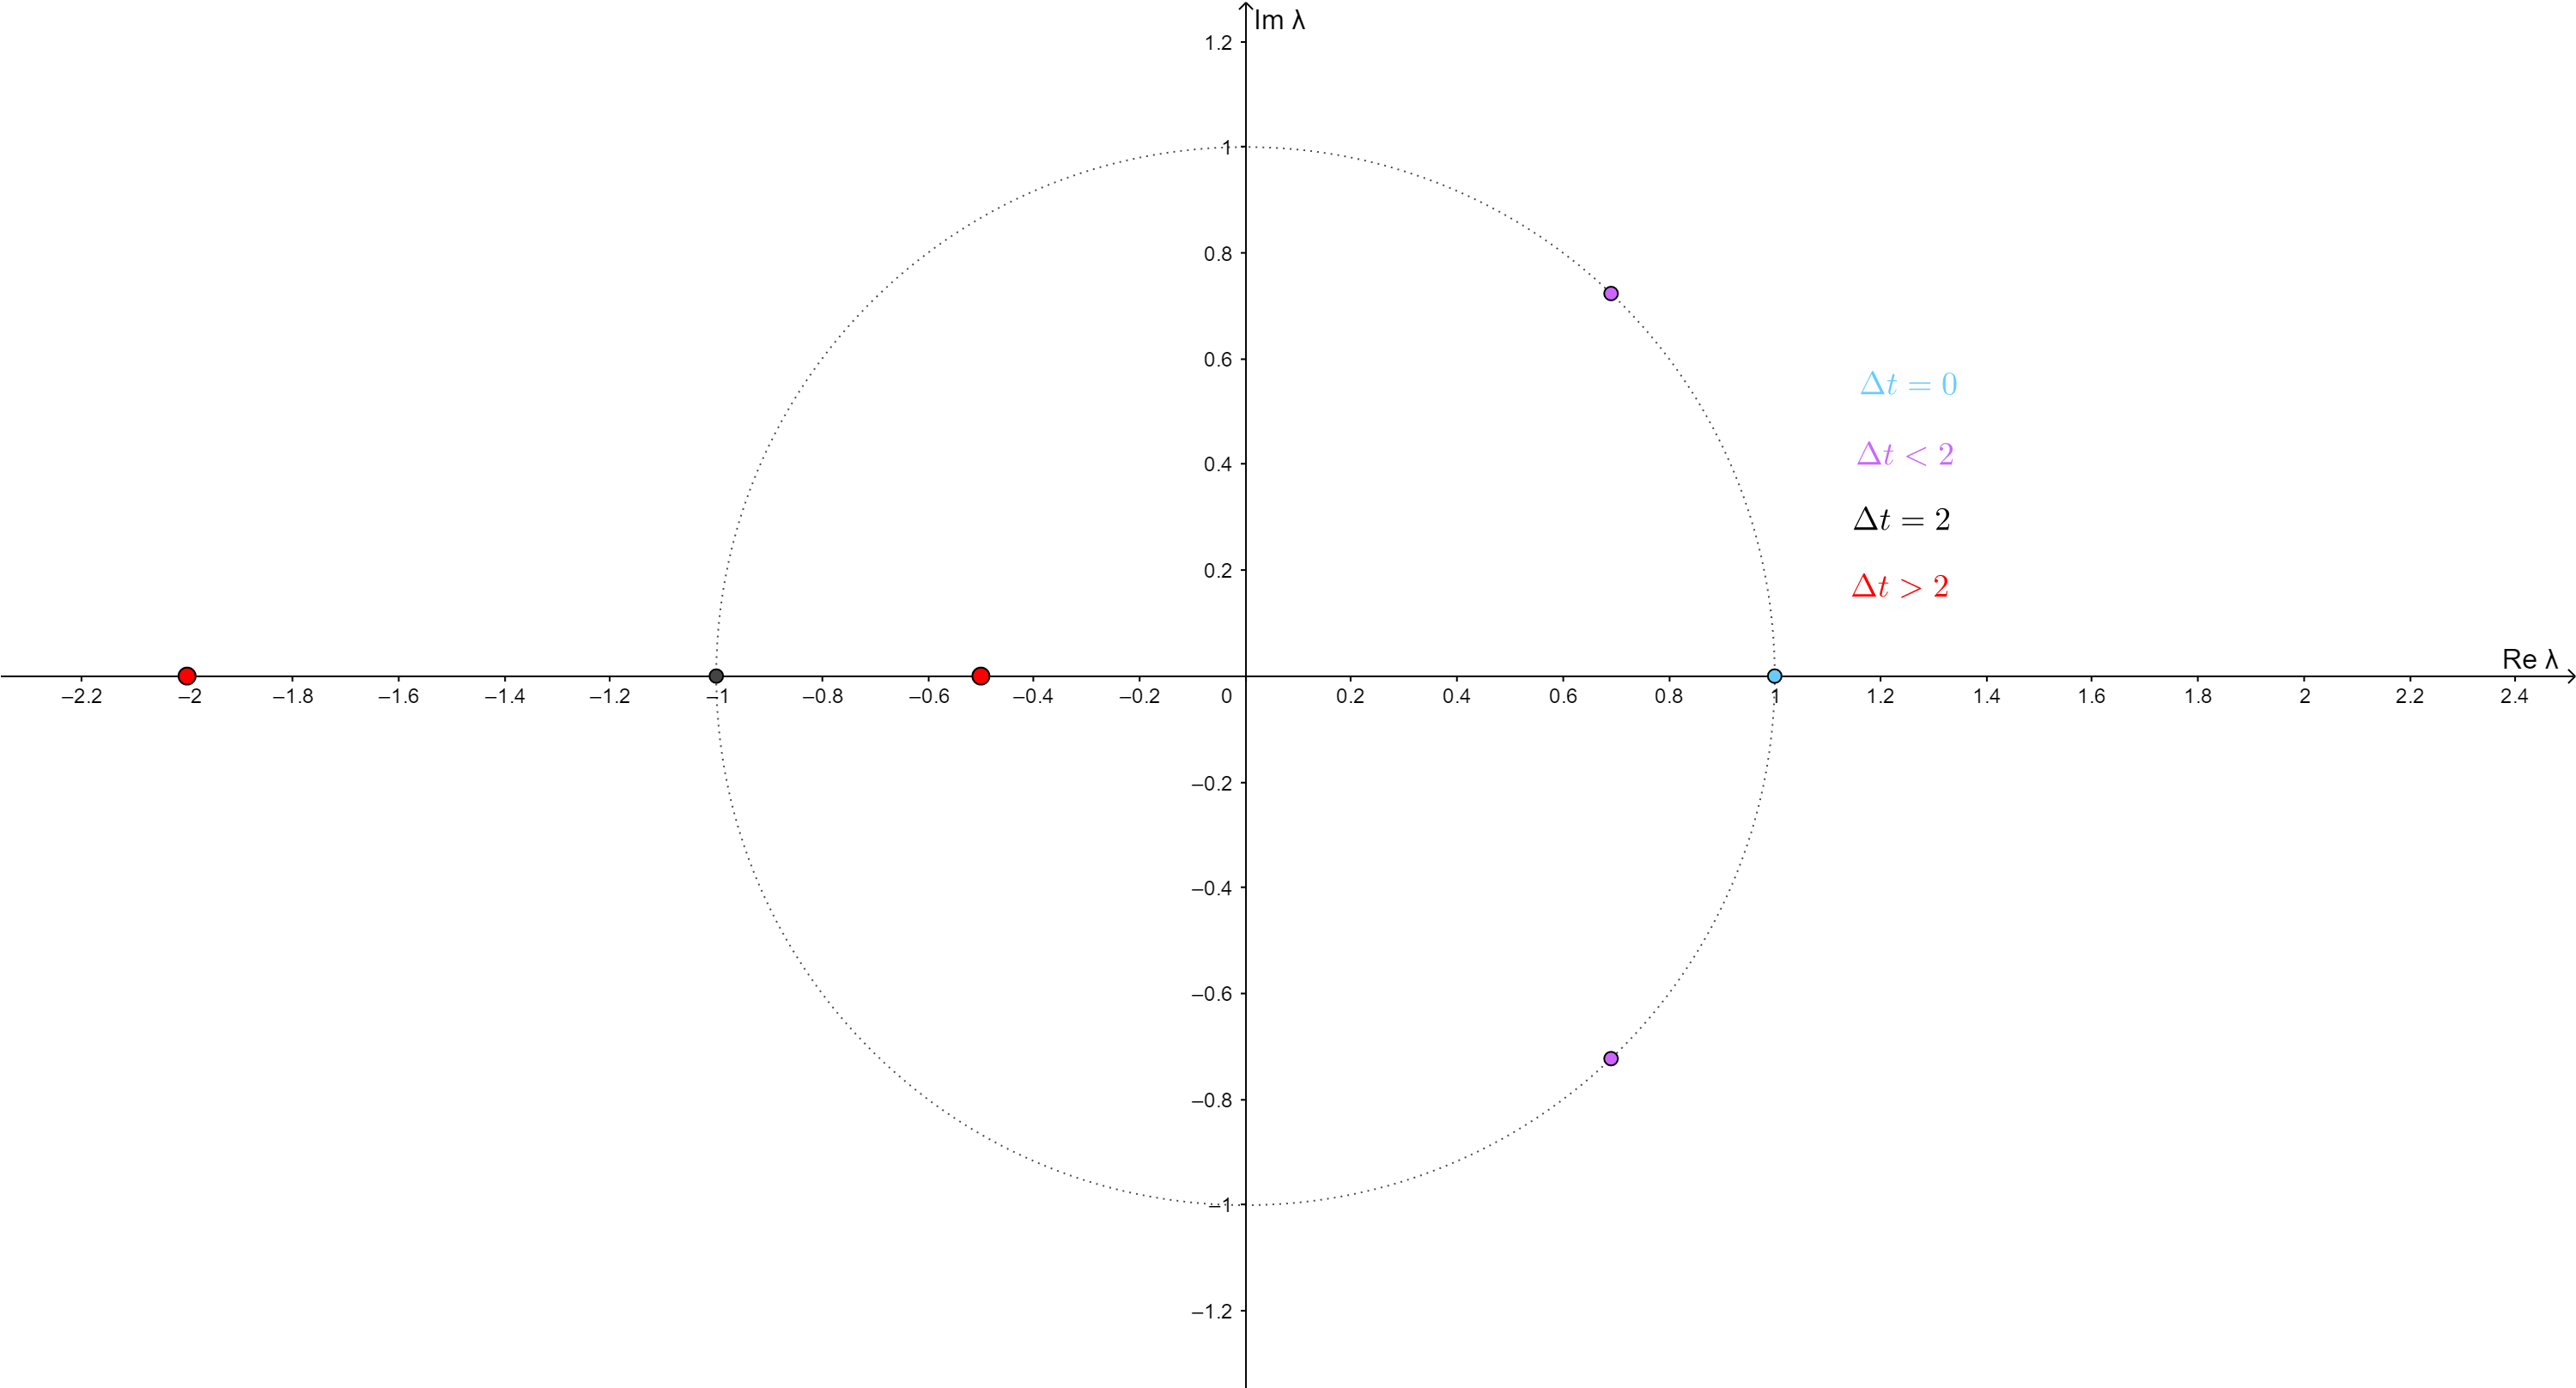
\includegraphics[scale=3.0]{Integrators/images/complexplane.png}
    \caption{Possible eigenvalues of the matrix $A$}
    \label{fig:complexplane}
\end{figure}
In the case where they are complex, their imaginary part is opposite and the real parts are equal.
After n steps:
\begin{equation}
    \begin{pmatrix}
      q' \\
      p'
    \end{pmatrix}
    = A^n
    \begin{pmatrix}
      q \\
      p
    \end{pmatrix}
\end{equation}
Check the behaviour for a large number of time steps ($n\xrightarrow{}\infty$):
\begin{itemize}
    \item if $A^n$ contains some infinite term, then the trajectory will diverge.
    \item if $A^n$ goes to 0, then the trajectory will converge (oscillate around the circular trajectory).
\end{itemize}
The eigenvalues of $A^n$ are equal to the eigenvalues of $A$ raised to the n-th power, therefore:
\begin{itemize}
    \item  $\lambda_1=\lambda_2=-1$: trajectory will oscillate\footnote{$\lambda_1=\lambda_2=1$ is the case when the timestep is equal to zero, therefore the system is not moving}. $$\Delta t = 2$$
    \item $\lambda_1> -1$, $\lambda_2< -1$ or $\lambda_2> -1$, $\lambda_1< -1$: matrix explodes, trajectory diverges. $$\Delta t > 2$$
    \item complex eigenvalues with unitary modulus: trajectory will oscillate.  $$\Delta t < 2$$
\end{itemize}
Threshold for stability of a numerical simulation:
\begin{equation}
    \Delta t < \frac{T}{\pi}
\end{equation}
This is the theoretical limit for the timestep, given the period. The criterion for the timestep is the same for Verlet and Velocity Verlet.
\subsection{Multiple springs}
Let us consider a situation where there are 3 particles with the same mass connected by springs with $k_1 >> k_2$. Let us estimate the maximum time step that should be used. The solution is to take the stiffest spring to impose the limit on the timestep, i.e., that gives the shortest timestep.
In general, this condition is given by the fastest degree of freedom, in other words, by the lightest possible atom with the stiffest spring. This is the way to find the upper bound for our timestep:
computing the period $2\pi \sqrt{\frac{m}{k}}$.
If energy is sufficiently conserved, this means that the timestep is small enough. It is difficult to predict a priori a good value of the timestep because there could be nonlinear potentials.


    \section{The Gran-Canonical ensemble}
Let's now consider a system for which the number of particles is allowed to fluctuate, as if the system were in contact with a larger system at the same temperature, with which it can exchange particles. In order to treat this case, we need to add to the phase space distribution function an extra index accounting for the number of particles N:
\begin{equation}
    \rho(\textbf{q},\textbf{p}) \rightarrow \rho_N(\textbf{q},\textbf{p}).
\end{equation}
A more general definition of Entropy may be written too:
\begin{equation}
        S = -k_B \sum_N \int \frac{d\Gamma_N}{h^{3N}}  \rho_N\ln{\rho_N},\label{S}
\end{equation}
  This corresponds to the most general integration over phase space of the expression $\rho_N\ln{\rho_N}$. $h^{3N}$ is a dimensional factor deriving from quantization of phase space. Being it a constant, we will neglect this factor from now on. Again, due to the maximum entropy principle, an expression for the density $\rho_N$ can be found maximizing entropy with the appropriate constraints:
\begin{itemize}
    \item $\sum_N \int d\Gamma_N  \rho_N = 1 \: \Rightarrow \: \text{normalization} $\\
    \item $\sum_N \int d\Gamma_N  \rho_N H_N = <E> \: \Rightarrow \: \text{mean energy conservation}\\$
    \item $\sum_N \int d\Gamma_N  \rho_N N = <N> \: \Rightarrow \: \text{mean n. of particles conservation}\\$
\end{itemize}
Hence, we're looking for $\rho_N^*$ such that the functional 
\begin{equation}
    \mathcal{F}[\rho_N] = -\sum_N\int d\Gamma_N \rho_N ( \ln{\rho_N} - \lambda + \beta H_N - \beta \mu N)
\end{equation}
is stationary. Imposing: 
\begin{align}
    \partial\mathcal{F}[\rho_N^*] &\equiv \mathcal{F}[\rho_N^*+\delta\rho_N] - \mathcal{F}[\rho_N^*]\\
    &\simeq -\sum_N\int d\Gamma_N \delta\rho_N(\ln{\rho_N^*}+1-\lambda+\beta H_N -\beta \mu N)=0
\end{align}
we get the following expression:
\begin{equation}
\label{eq:rho_micro}
    \rho_N^*=\frac{e^{-\beta(H_N-\mu N)}}{Z_{GC}}\:. 
\end{equation}
An \textit{ad hoc} extra factor $1/N!$ has to be introduced to obtain the correct additive Entropy (see Huang), so that the final result is:
\begin{equation}\label{incriminate} 
    \rho_N^*=\frac{e^{-\beta(H_N-\mu N)}}{N! Z_{GC}},\hspace{0.5 cm} \text{with} \: Z_{GC}= \sum_N\int d\Gamma_N \frac{e^{-\beta(H_N-\mu N)}}{N!}.
\end{equation}
The new Lagrange multiplier we have introduced, $\mu$, is called \textit{chemical potential}. We will later give an interpretation for it.\\

\textit{\textbf{Comment:} I believe Micheletti was imprecise here. In eq.\ref{incriminate} the factor $1/N!$ should be present in the expression for $Z$ but not in the one for $\rho$. Actually, if both expressions contained it, we would be multiplying $\rho$ for a $N!/N!=1$ factor and eq.\ref{S} would remain unchanged. The correct interpretation is the following: being atoms quantum mechanically indistinguishable, any permutation of the atoms indexes does not produce a new state of the system. Then the factor $1/N!$ accounts for the fact that an infinitesimal volume $dpdq$ in phase space corresponds to $dpdq/N!$ different micro-states only. In conclusion, when taking averages of functions $f(p,q)$ over the possible micro-states of the system, we should write integrals as:
\begin{equation}
    <f> = \sum_N \int \frac{d\Gamma_N}{N!h^{3N}}  \rho_N f(q,p).
\end{equation}
This explains why $1/N!$ is only present in the expression for $Z$. Also, computing entropy like this all factors $1/N!$ simplify apart from the one inside the logarithm, so that we obtain the correctly rescaled expression.
}\\

As an example, we can compute the Gran-Canonical partition function $Z_{GC}$ for an ideal gas:
\begin{equation}
    \begin{split}
    Z_{GC} &= \sum_N \frac{1}{N!}\int d\Gamma_N e^{-\beta(H_N-\mu N)}\\
    &=\sum_N \frac{e^{\beta \mu N}}{N!}\int d\Gamma_N e^{-\beta H_N}\\
    &=\sum_N \frac{e^{\beta \mu N}}{N!}V^N\biggl( \frac{2\pi m}{\beta}\biggr)^{3N/2}\\
    &=\sum_N \frac{x^N}{N!}=e^x, \hspace{0.5 cm} \text{with} \:x=e^{\beta \mu}V \biggl(\frac{2\pi m}{\beta}\biggr)^{3/2}.
    \end{split}
\end{equation}
We have used the expression \ref{eq:zcannone} for the Canonical partition function computed in the previous section. We call the factor $z=e^{\beta \mu}$ \textit{fugacity}. The mean number of particles $<N>$ can be computed too. Being $Z_{GC}$ a cumulant generating function, 
\begin{equation}
    <N>=\frac{\partial ln Z_{GC}}{\partial (\beta \mu)}
    =e^{\beta \mu}V \biggl(\frac{2\pi     m}{\beta}\biggr)^{3/2}. \label{eq.N}
\end{equation}
Consequently:
\begin{equation}
   \begin{split}
    & e^{-\beta \mu}=\frac{V}{<N>}\biggl(\frac{2\pi m}{\beta}\biggr)^{3/2} \\
    & \mu=-K_B T ln \biggl[\frac{V}{<N>}\biggl(\frac{2\pi m}{\beta}\biggr)^{3/2} \biggr].
    \end{split}
\end{equation}
The equation we have obtained for $\mu$ tells us something important about its physical interpretation. Recalling the equation for the \textit{free energy} for a canonical ensemble in the case of an ideal gas,
\begin{equation}
    \begin{split}
    F_{CAN}&=-k_B T \ln{Z_{CAN}}\\
    &=-k_B T ln\biggl[ \frac{V^N}{N!}\left(\frac{2\pi m}{\beta} \right)^{3N/2}\biggr]\\
    &=-k_B T \biggl[N\ln{V}-ln(N!)+\frac{3N}{2}\ln{\left(\frac{2\pi m}{\beta} \right)}\biggr]\\
    &\simeq -k_B T \biggl[N\ln{V}-(NlnN-N)+\frac{3N}{2}\ln{\left(\frac{2\pi m}{\beta} \right)}\biggr],\\
    \end{split}
\end{equation}
where we have used Stirling's approximation, we have that:
\begin{equation}
   \frac{\partial F_{CAN}}{\partial N}=-K_B T ln \biggl[\frac{V}{N}\biggl(\frac{2\pi m}{\beta}\biggr)^{3/2} \biggr]=\mu.
\end{equation}
In conclusion, $\mu$ corresponds to the difference in \textit{free energy} due to variations of the number of particles the system is composed of.

\subsection{Equilibrium condition for chemical reactions}
The \textit{chemical potential} $\mu$ turns out to be very useful in some chemistry problems. Let's consider a generic chemical reaction involving n reactants and m products:
\begin{equation}
    \nu_1 x_1 + ... + \nu_n x_n \rightleftharpoons \nu_{n+1} x_{n+1} + ... + \nu_{n+m} x_{n+m}
\end{equation}
Clearly, when elements react, the number of molecules $N_i$ of element i varies: $N_i \rightarrow N_i+\delta N_i$. This makes the system we're studying a Gran-Canonical one. On the other hand, starting from equilibrium, the ratio $\delta N_i/\nu_i$ between the variation of the number of molecules of element i and its stoichiometric coefficient must be constant and equal for all i's. Also, if the system keeps at equilibrium the \textit{free energy} F must be minimal. Then:
\begin{equation}
    \begin{split}
    \partial F &= F(N_1+\delta N_1,...,N_{n+m}+\delta N_{n+m})-F(N_1,...,N_{n+m})\\
    &=\frac{\partial F}{\partial N_1}\delta N_1+...+\frac{\partial F}{\partial N_{n+m}}\delta N_{n+m}\\
    &=\mu_1 \delta N_1+...+\mu_{n+m} \delta N_{n+m}=0.
    \end{split}
\end{equation}
Knowing $\delta N_i/\nu_i= const=\delta N$, with $\delta N$ arbitrary, we get to the equilibrium condition:
\begin{equation}
    \sum_i \mu_i \nu_i=0.
\end{equation}
Notice that, for convention, stoichiometric coefficients $\nu_i$ are positive for reactants and negative for products. This same condition may be written in terms of the fugacity $z$ as:
\begin{equation}
    e^{\beta\sum_i \mu_i \nu_i}=\prod_i (z_i)^{\nu_i}=1.\label{eq.fugacity}
\end{equation}
From eq.\ref{eq.N}:
\begin{equation}
    z=\bigl[ v \bigl( \frac{2\pi m}{\beta}\bigr)^{3/2}\bigr]^{-1}, 
\end{equation}
where $v=\frac{V}{N}$ is the concentration of the $i_{th}$ element. Then eq.\ref{eq.fugacity} tells us:
\begin{equation}
    \prod_i v_i^{\nu_i}\sim\prod_i (m^{\nu_i})^{-3/2}.  
\end{equation}
This is known as the law of mass action, stating that the the quantity $\prod_i v_i^{\nu_i}$ is a constant for reactions at equilibrium, namely the \textit{equilibrium constant}.  
\chapter{Integrators}
    \section{Introduction}
In molecular dynamics, a thermostat is an algorithm built with the purpose of generating samples from a statistical ensemble at constant temperature $T$.
At this point, we know that the typical choice among the statistical ensembles, when simulating a real physical system, is the Canonical one, which allows fluctuations of the total energy under the constraint that its average remains constant over time.
Therefore, our aim will be to build thermostats which sample configurations drawn from the Canonical ensemble. 

Before entering in the implementation of these algorithms, let's recall some of the main features of the ensemble we are interested in.

\subsection{Recap of the Canonical ensemble}
The probability distribution related to the Canonical ensemble, as defined in Chapter 1 (1.36), is given by
\begin{equation}
     P(x)=\frac{e^{-\beta H(x)}}{Z}
\end{equation}
with 
\begin{equation}
     Z=\int_ {}^{} e^{-\beta H(x)}dx
\label{zetafunc}
\end{equation} 

\par Is important to remember that here $x$ represents a vector that contains the position and momenta of all the particles of the system, so the integral (5.2) is taken over all the points composing the phase space of our system. 

As we have already seen, this formulation allows us to compute the average of a generic observable $A(x)$ as
\begin{equation}
     \langle A \rangle =\int_ {}^{} P(x)A(x)dx,
\end{equation}

and, as a consequence, its variation with respect to the temperature as
\begin{equation}
    \frac{\partial \langle A \rangle}{\partial T}=-\frac{1}{k_B T^2} (-\langle HA \rangle+\langle H \rangle\langle A\rangle). 
\end{equation}

Some relevant examples are the derivatives of the average values of:
\begin{itemize}
    \item The total energy $H$
    \begin{equation}
      \frac{\partial \langle H \rangle}{\partial T}=\frac{1}{k_B T^2} (\langle H^2\rangle-\langle H\rangle^2)=\frac{1}{k_B T^2}\sigma_H^2
    \end{equation} 
    which is proportional to the variance of $H$ (i.e. the amplitude of its fluctuations) and which can be physically interpreted as the amount of energy needed in order for the temperature to increase by 1 degree, i.e. the Heat capacity; 
    \item The potential energy $U$
    \begin{equation}
        \frac{\partial \langle U \rangle}{\partial T}=\frac{1}{k_B T^2} (\langle U^2 \rangle -\langle U \rangle^2)=\frac{1}{k_B T^2}\sigma_U^2 ;
    \end{equation}
    \item the kinetic energy $K$
    \begin{equation}
        \frac{\partial \langle K \rangle}{\partial T}=\frac{1}{k_B T^2} (\langle K^2\rangle-\langle K \rangle^2)=\frac{1}{k_B T^2}\sigma_K^2 .
    \end{equation}
\end{itemize}

In particular, the last two results are obtained exploiting the feature of the Hamiltonian of the majority of the systems we are interested in, built as the sum of a kinetic contribution \begin{math} K(p)=\sum_{i=1}^{N_a} \frac{{p_i}^2}{2m_i} \end{math}, which depends only on the momenta $p_i$ of the particles, and a potential contribution $U(q)$, specific of the system, which depends only on the positions $q_i$. 

This composition of the Hamiltonian makes the probability distribution $P(x=p,q)$ factorizable into two separate parts: \begin{math}P_K(p) \propto e^{-\beta \sum_{i=1}^{N_a} \frac{p_i^2}{2m_i}} \end{math} (which is a gaussian) and $P_U(q)$.

Then, from  $P_K(p)$ we can obtain the probability distribution of the kinetic energies $P_K(K)$, which is not a gaussian (because as $K<0$, $P_K$ is identically equal to $0$), but a Gamma distribution
\begin{equation}
    P_K(K) \propto K^{N_F/2 -1}e^{-\beta K}
\end{equation}
where $N_F=3N_a$ is the number of degrees of freedom, with average
\begin{equation}
    <K>=\frac{3}{2} N_a k_B T \implies \frac{\partial <K>}{\partial T}=\frac{3}{2} N_a k_B
\end{equation}

and width (from (5.7) and (5.8))
\begin{equation}
    \sigma_K=\sqrt{k_B T^2 \frac{\partial <K>}{\partial T}}=\sqrt{\frac{3}{2} N_a k_B^2 T^2}= \sqrt{<K>^2 \frac{2}{3 N_a}}.
\end{equation}
In particular, the factor $K^{N_F/2 -1}$ is in some way related to the density of state: this explains why negative kinetic energies are not allowed ($P_K(K<0)=0$) and why, without the compensation of the Boltzmann factor \begin{math} e^{-\beta K} \end{math}, high kinetic energies would be more likely.
A qualitative description of the behaviour of $P_K(K)$ can be seen in Figure \ref{fig:kinetic distribution}

\begin{figure}
    \centering
    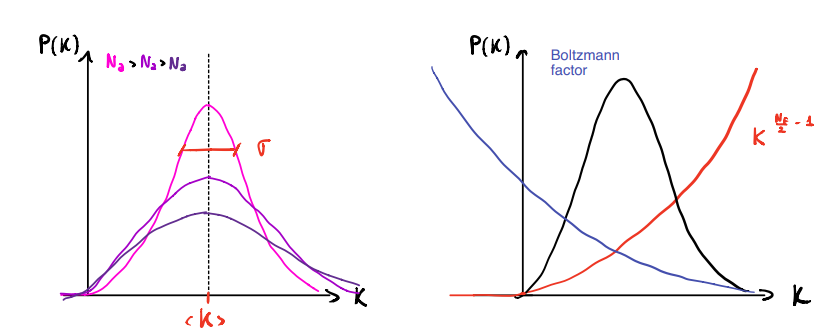
\includegraphics[width=0.7\textwidth]{Thermostats/images/kinetic distribution.PNG}
    \caption{On the left: qualitative behaviour of the Gamma distribution $P_K(K)$ at different values of $N_a$, always centered in the same value in order to compare visually the different shapes. On the right: qualitative behaviour of the two factors that compose $P_K(K)$, whose coexistence leads to the typical shape of the Gamma distribution.}
    \label{fig:kinetic distribution}
\end{figure}

\section{Algorithms}

As mentioned in the Introduction, the two main properties of the thermostats we want to implement are:
\begin{itemize}
    \item Equilibration of the system to a target value of the temperature $\bar T$, that, after an early transient, have to remain constant;
    \item Production of configurations drawn from the Canonical ensemble.
\end{itemize}

First of all, we have seen, as one of the main results of the theoretical description of the Canonical ensemble, that \begin{math} <K> \propto T \end{math}. 
Therefore, we can think about controlling the value of the temperature through the control of the kinetic energy $K(p)$, which will have to reach the target value $\bar K \propto \bar T$. This control on $K(p)$ can be realized imposing proper variations of $K(p)$ itself, in such a way that $<K>= \bar K$. 

But this will not be sufficient in order to satisfy the second request: in fact, in order for our simulation to produce canonical configurations, we need also the fluctuations on $K(p)$ to be coherent with the canonical distribution, and so equal to its variance $\sigma_K^2$.

As a consequence of these requirements, the main idea to implement thermostats is by choosing a rule for the variation of $K(p)$, and evolving the system through a modified version of Hamilton equations, which will determine variations of potential energy $U(q)$ in such a way that the ones of $K(p)$ are balanced, and so that the total energy is approximately conserved.


\subsection{Trial and error}

The first attempt, which can not be called an actual algorithm, but is useful to introduce us to the logic underlying thermostats, is the "Trial and error". 
It exploits the behaviour of the simulation to set the proper value of the initialization $K_0$ which, after a transient, will lead to the target value \begin{math} \bar K \end{math} (and so to the target value \begin{math} \bar T \end{math}).

At first, in fact, we could try initializating the kinetic energy at its target value. Unfortunately, starting the simulation we would see that $K$ doesn't remain constant at $\bar K$, but equilibrates to a different value.

So, we could think of starting a new simulation from a different $K_0$, shifted from the previous by the difference between $\bar K$ and the previous equilibration value.
Typically, the optimal result can not be reached in a unique attempt, but after various iterations, which can be stopped when the difference between $\bar K$ and the new equilibration value of $K$ is small enough.

\begin{figure}
    \centering
    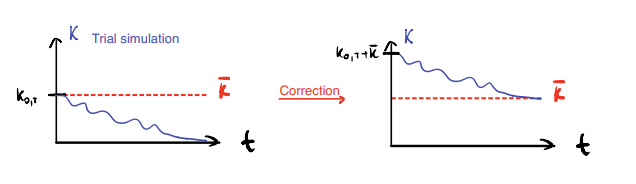
\includegraphics[width=0.7\textwidth]{Thermostats/images/Trial and error.PNG}
    \caption{The first image represent the Trial simulation, where the kinetic energy is initialized to its target value. The second represent the correct simulation, where the initialization is set to that value from which, after the equilibration, the kinetic energy reaches the target value.}
    \label{fig:trial and error}
\end{figure}

In Figure \ref{fig:trial and error} we see how this procedure would look if a unique attempt would be sufficient.

Unfortunately, as we can imagine looking at the triviality of this algorithm, this is not a suitable choice for implementing a thermostat.

\subsection{Velocity rescaling}
The Velocity rescaling algorithm is based on the following idea:
\begin{itemize}
    \item Given an initial configuration of the system, we run a number \textit {stride} of steps using a Hamilton equations integrator, like, for example, Velocity Verlet;
    \item We check the istantaneous value of $K$ and we change it rescaling it by a factor that makes it equal to the target value $\bar K=\frac{3}{2}N_a K_B \bar T$.
\end{itemize}

A pseudocode representing these operations would be:
\begin{algorithm}[H]\label{velocity_rescaling}
			\caption{Velocity rescaling algorithm}
			\begin{algorithmic}[1]
				\For{$i step\; inrange (nsteps)$}
    				\State $p+=f*\Delta t/2$
    				\State $q+=p*\Delta t/m$
    				\State $p+=f*\Delta t/2$
    				\If{$i step\%stride==0$}
    				    \State $K= \frac{\sum_{i}{p_i^2}}{{2m_i}}$
    				    \State $p* = \sqrt{\frac{\Bar{K}}{K}}$
    				\EndIf
				\EndFor
			\end{algorithmic}
		\end{algorithm}

\begin{figure}
    \centering
    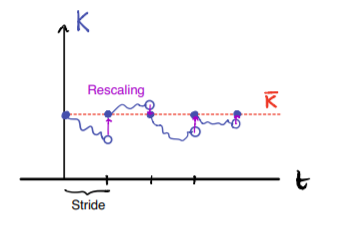
\includegraphics[width=0.7\textwidth]{Thermostats/images/velocity rescaling.PNG}
    \caption{Example of a trajectory $K(t)$ produced using the Velocity rescaling thermostat.}
    \label{fig:velocity rescaling}
\end{figure}		

As we can see, in this case the change in the kinetic energy is made on its total value, and not on the specific values $K_i$ of the single particles: this feature defines the so called \textit {Global thermostats}.

Although, as also qualitatively represented in Figure \ref{fig:velocity rescaling}, this algorithm works well in the equilibration to the target value $\bar K$, reached in a time interval $\propto {\textit {stride}}$, this is not an optimal choice for two main reasons: first of all, the distribution we are sampling from is unknown, and certainly it is not the canonical since the fluctuations of $K$ are not the proper ones (see Figure \ref{fig:fluctuations}); then, the trajectory is discontinuous, and this does not allow us to convert the algorithm into a differential equation.

\begin{figure}
    \centering
    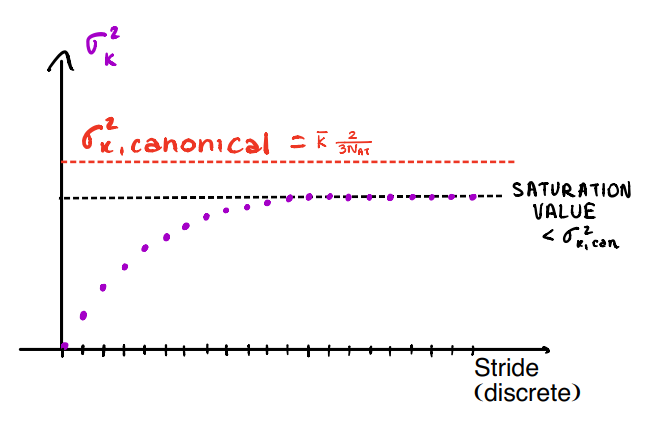
\includegraphics[width=0.7\textwidth]{Thermostats/images/fluctuations.PNG}
    \caption{Behaviour of $\sigma_K^2$ as a function of \textit {stride}. If \textit {stride} is small, the trajectory is smoother and $<K>=\bar K$, but the fluctuations are too small. If \textit{stride} is too big, the fluctuations will reach a saturation value smaller than the correct one, and also $K$ doesn't reach the target: in fact, this choice would basically correspond to evolving the system according to Velocity Verlet, which guarantees the conservation of the total energy and then produces configurations drawn from the Microcanonical distribution. }
    \label{fig:fluctuations}
\end{figure}

\subsection{Berendsen thermostat}
The problem of discontinuity in Velocity rescaling algorithm is soon solved by the Berendsen thermostat, which can be interpreted as its "continuous version".

It is based on the idea of modifying $K$ at each step, rescaling it by a properly weighted sum of the current value and the target value.

In practice, this operation would consist into the multiplication of the current value of the momentum $p$ by a factor
\begin{equation}
    F={\sqrt{\frac{c_1K+c_2 \bar K}{K}}}.
\end{equation}

In particular, the choice of the weights ${c_1}$ and ${c_2}$ has to guarantee the following properties:
\begin{itemize}
    \item $c_1+c_2=1$
    since, when $K=\bar K$, the factor F must be equal to 1, because the target value has been reached, and then we do not have to modify the current value;
    \item the limit $c_1 \rightarrow 1$ ( $\implies c_2 \rightarrow 0$), which represents the absence of the thermostat (since there are no corrections to the current values $p$) should coincide with the limit case of $\textit{stride}=\tau \rightarrow \infty$ in Velocity rescaling;
    \item the limit $c_2 \rightarrow 1$ ($\implies c_1 \rightarrow 0$), which basically respresents the application of Velocity rescaling at each step, should coincide with the limit case of $\textit{stride}=\tau \rightarrow 0$.
\end{itemize}

A choice which guarantees the latter requests is:
\begin{equation}
   c_1=e^{-{\frac{\Delta t}{\tau}}} ;\quad
      c_2=1-c_1=1-e^{-{\frac{\Delta t}{\tau}}}
\end{equation}

At this point, we can try converting the algorithm into a differential equation:
\begin{multline*}
    K_{new}={\frac{e^{-{\frac{\Delta t}{\tau}}}K+\left(1-e^{-{\frac{\Delta t}{\tau}}}\right) \bar K}{K}}K \\ 
    \implies \Delta K=K_{new}-K=e^{-{\frac{\Delta t}{\tau}}}K + (1-e^{-{\frac{\Delta t}{\tau}}}) \bar K - K \\
    = (1-e^{-{\frac{\Delta t}{\tau}}} )(\bar K -K) 
\end{multline*}

Then, performing the infinitesimal limit:
\begin{equation*}
    \lim_{{\Delta t}\to 0} \Delta K = (1-1+\frac{\Delta t}{\tau} + \textit{h.o.t})(\bar K-K)=\frac{\Delta t}{\tau}(\bar K-K)
\end{equation*}

\begin{equation}
    \implies dK=dt \frac{(\bar K-K)}{\tau}
\end{equation}

that is actually a differential equation. This means its solution, i.e. $K(t)$, is continuous, and then we can say that the issue we had with Velocity rescaling is solved.

Another advantage with respect to Velocity rescaling is that now we have a control parameter $\tau$, which, differently from \textit{stride}, has a physical interpretation:
it is the relaxation time of the system, and gives a qualitative measure of the thermal inertia of it, since the greater is $\tau$, the more difficult will be to change $K$, namely $T$.

Moreover, as a smoother version of Velocity rescaling, Berendsen's is itself a global thermostat.

So, in conclusion, one of the main advantages of using this algorithm is that the trajectories it produces are continuous, but it is not the only one. In fact, according to the huge number of citations of the original paper by Berendsen (1984), it is probably the most used thermostat, and this is due to a series of properties: it empirically equilibrates well; it is easy to understand; it is efficient. Regarding the efficiency, this is what actually makes people prefer this algorithm to more exact ones like, for example, Hybrid Montecarlo: indeed, the approximation makes Berendsen thermostat quicker in simulating very large systems, for  which a more accurate algorithm would take a too long time.

However, this algorithm does not sample configurations from the canonical distribution. In fact, even if balance is satisfied, because a stationary distribution can be reached, this is not the canonical one, and this is due to the fact that $K$ does not respect the proper fluctuations. Detailed balance is instead not guaranteed, because $K$ is forced to reach $\bar K$ and a time-reversed trajectory is not even possible.




    \section{Maximum entropy principle and microcanonical ensemble}
As before, consider a system divided in two compartments with energies $E_1$ and $E_2$. The two subsystems can exchange energy, but the sum $E_1+E_2 = E$ is fixed. We have already demonstrated that the phase space of the system at the equilibrium is given by 
\begin{equation}
    \Gamma_{1+2}(E) = \Gamma_1(E_1^*)\,\Gamma_2(E-E_1^*),
\end{equation}
where $E_1^*$ is the energy that maximizes $\Gamma_{1+2}$. This relation is clearer if one thinks of $\Gamma_i$ as the degeneracy of a state with an energy $E_i$. The equilibrium condition then becomes
\begin{equation}
    \frac{\partial \Gamma_{1+2}}{\partial E_1}\bigg|_{E_1^*} = \frac{\partial \Gamma_1(E_1)}{\partial E_1} \Gamma_2(E - E_1) + \Gamma_1(E_1)\frac{\partial \Gamma_2(E - E_1)}{\partial E_1} = 0.
\end{equation}
Since we have the constraint $E_2 = E-E_1$, we can take the derivative of $\Gamma_2$ with respect to $E_2$, changing its sign. Ordering the terms and multiplying by the Boltzmann constant $k_B$ we obtain
\begin{equation}
    \frac{k_B}{\Gamma_1} \frac{\partial \Gamma_1}{\partial E_1} = \frac{k_B}{\Gamma_2} \frac{\partial \Gamma_2}{\partial E_2} \: \Longrightarrow \:
    k_B \frac{\partial (\ln{\Gamma_1})}{\partial E_1} = k_B \frac{\partial (\ln{\Gamma_2})}{\partial E_2}
\end{equation}
and $k_B\ln{\Gamma}$ was our definition of entropy $S$. So the equilibrium condition is 
\begin{equation}
    \frac{\partial S_1}{\partial E_1} = \frac{\partial S_2}{\partial E_2}
\end{equation}
which is equivalent to having the same temperature. \\ \\

Entropy is an observable, so its expected value can be written as $S = \int d\Gamma \rho f(q,p)$ for a certain function $f$ of positions and momenta. From an analogy with probability theory and Shannon entropy, entropy turns out to be
\begin{equation}
    S = -\int d\Gamma \rho \ln{\rho}.
\end{equation}
which is also equal to $S=\ln{\Gamma}$ (for $k_B=1$).
We don't give a formal proof of this statement, but we show that it gives correct results in two particular limit cases:
\begin{itemize}
    \item case 1: $n$ energy levels, with $p_1 = 1$ and $p_{i\neq 1} = 0 \: \Rightarrow \: S=0$. \\
    \item case 2: $p_i = 1/n$ for all $i \: \Rightarrow \: S= -\frac{1}{n}\ln(\frac{1}{n})^n = \ln{n}$.
\end{itemize}
The maximum entropy principle states that a system in equilibrium tends to maximize entropy, given the constraints, for every probability density $\rho$. For the microcanonical ensemble, we consider the following constraints for $\rho$:
\begin{gather}
    \int d\Gamma \rho = 1 \: \Rightarrow \: \text{normalization} \\
    \rho(\mathbf{q},\mathbf{p}) = 0 \: \text{if} \: H(\mathbf{q},\mathbf{p}) \not\in (E,E+\Delta).
\end{gather}
For $k_B=1$, $S = -\int d\Gamma \rho \ln{\rho}$ and introducing the Lagrange multiplier $\lambda$ we can construct the functional
\begin{equation}
    \mathcal{F}[\rho] = -\int d\Gamma (\rho \ln{\rho} - \lambda\rho)
\end{equation}
and our goal is to find $\rho^*$ that makes it stationary. More explicitly, we want the functional differential
\begin{equation}
    \partial\mathcal{F}[\rho^*] \equiv \mathcal{F}[\rho^*+\delta\rho] - \mathcal{F}[\rho^*]
\end{equation}
with no linear terms in $\delta\rho$. Then we get
\begin{align}
\label{eq:rho_micro}
    \partial\mathcal{F}[\rho^*] &= -\int d\Gamma [(\rho^*+\delta\rho)\ln(\rho^*+\delta\rho) - \lambda(\rho^*+\delta\rho)] + \int d\Gamma (\rho^*\ln\rho^* - \lambda\rho^*) \nonumber \\
    &= -\int d\Gamma (\delta\rho\ln{\rho^*}+\delta\rho-\lambda\,\delta\rho) + h.o.t. \nonumber \\
    &= -\int d\Gamma \delta\rho \,(\ln{\rho^*}+1-\lambda) = 0
\end{align}
where in the second line we have used the fact that 
\begin{equation}
    \ln(\rho^*+\delta\rho) \simeq \ln{\rho^*} + \frac{\delta\rho}{\rho^*} + h.o.t.
\end{equation}
Since eq. (\ref{eq:rho_micro}) has to hold for every $\delta\rho$, the integrand must be null, i.e.
\begin{equation}
    \ln{\rho^*}(\mathbf{q},\mathbf{p}) = \lambda-1
\end{equation}
that does not depend on $\mathbf{q}$ and $\mathbf{p}$, so we obtain a uniform \textit{a priori} probability. This is due to the fact that we had no constraints, except for the normalization of the probability density. We can repeat the same calculation adding the constraint 
\begin{equation}
    \int d\Gamma \rho\,H = \bar{E}
\end{equation}
that corresponds to the canonical ensemble.




    %by Elena C. WORK IN PROGRESS
\subsection{Leapfrog Algorithm}
The Velocity Verlet algorithm shown previously (Algorithm \ref{alg:velocity_verlet}) can be modified to reduce the computational cost.\\ In particular, compute a force is quite expensive: computing the force twice will require twice the simulation time. One solution to reduce the computational cost is to merge the momenta shifts together (using the same value of the force): this leads to a slightly faster simulation, but on the other side this kills the possibility of printing the values of p and q at the same time (access to the phase space). This solution is called \textbf{Leapfrog algorithm}.\\
\begin{algorithm}[H]
			\caption{Leapfrog algorithm}
			\label{alg:leapfrog}
			\begin{algorithmic}[1]
			    \State $p=p+f*\Delta t/2$	\For{$i=1,...,nsteps$}
    			\State	$q=q+p/m \Delta t$
                 \State	$f=force(q)$
    			\State	$p=p+f*\Delta t$
				\EndFor
			\end{algorithmic}
		\end{algorithm}
Momentum and position are moved in an alternate way: at the end of a cycle, we do not find the values of the positions and momenta at the same timestep, they are found at a difference of half timestep. Slightly faster than Velocity Verlet, not very significant. 
\begin{figure}[H]
    \centering
    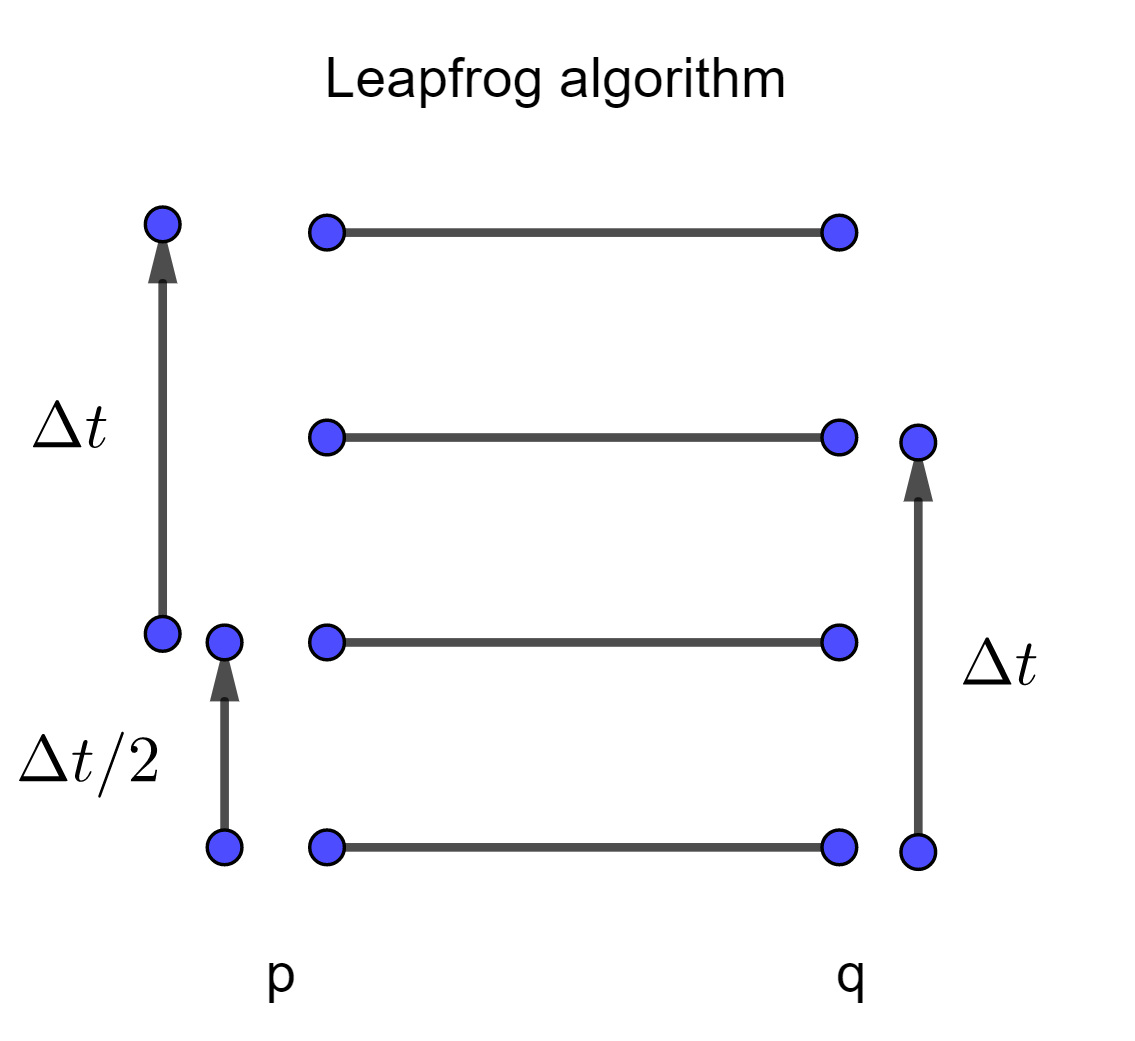
\includegraphics[width=50mm,scale=0.5]{Integrators/images/leapfrog.png}
    \caption{Scheme of the leapfrog algorithm}
    \label{fig:leapfrog}
\end{figure}
\subsection{Position Verlet}
Another alternative to the Velocity Verlet algorithm it is the so-called \textbf{Position Verlet algorithm}.
\begin{algorithm}[H]
			\caption{Position Verlet}
			\label{alg:position_verlet}
			\begin{algorithmic}[1]
        	\For{$i=1,...,nsteps$}
			\State	$q=q+p/m* \Delta t/2$
			\State	$f=force(q)$
			\State	$p=p+f*\Delta t$
			\State	$q=q+p/m* \Delta t/2$
				\EndFor
			\end{algorithmic}
		\end{algorithm}
This algorithm is the swapped version of Velocity Verlet, where the free particle is evolved for half timestep, then the infinite mass system is evolved for one timestep, then the free particle again for half timestep. 
\begin{itemize}
    \item \textbf{Advantages:} the force is computed only once, which is computationally advantageous (only one update of the momentum).
    \item \textbf{Disadvantages:} I cannot print the total energy. Potential energy needs to be computed with a similar procedure to the computation of forces (very expensive). Therefore, it is more convenient to compute forces and energies at the same time, but it is not possible with Position Verlet. Moreover, this algorithm is less used than Velocity Verlet, which is the simplest one.
\end{itemize}

\subsection{Other considerations on the Velocity Verlet algorithm}
Let us recall the Velocity Verlet algorithm:
    \begin{equation}\label{velocityverlet}
            \begin{cases}
                q(t+\Delta t)= q(t)+\frac{p(t)}{m}\Delta t+ \frac{f(t)}{m}\frac{\Delta t^2}{2}\\
                p(t+\Delta t)= p(t)+\frac{f(t)}{2}\Delta t+ \frac{f(t+\Delta t)}{2}\Delta t
            \end{cases}
            \end{equation}
Let's prove that the trajectories obtained with Velocity Verlet are equivalent to those obtained with Verlet algorithm. Trajectories are exactly time reversible, which means that we are allowed to compute $q(t-\Delta t)$ changing the sign of $\Delta t$ in the first equation \ref{velocityverlet}:
\begin{equation}\label{t-dt}
q(t-\Delta t)= q(t)-\frac{p(t)}{m}\Delta t+ \frac{f(t)}{m}\frac{\Delta t^2}{2}
\end{equation}
Let us sum $q(t-\Delta t)$ and $q(t+\Delta t)$ (first eq. \ref{velocityverlet} and eq. \ref{t-dt}):
\begin{equation*}
    q(t-\Delta t)+q(t+\Delta t)=2q(t)+\frac{f(t)}{m}\Delta t^2
\end{equation*}
This is consistent because equation \ref{velocityverlet} for the positions resembles a Taylor expansion of q.  The introduction of operator formalism is significant only for the sake of studying the evolution of momenta, while the evolution of positions is equivalent to the one obtained with the Verlet algorithm. 
In fact, the same trajectory results from the application of Verlet and Velocity Verlet algorithms.\\
Differences between the two algorithms are found by the fact that the Verlet algorithm considers differences between positions (current position $q(t_0)$ minus previous position $q(t_0-\Delta t$)): this leads to large round-off errors. Meanwhile, this problem is not present in Velocity Verlet, which is more numerically stable. Moreover, Velocity Verlet already includes a definition of the velocity, not present in Verlet algorithm: in the former case it is possible to compute the total energy and check if it is conserved.
We recall the properties of Velocity Verlet already discussed in section \ref{chapt:properites_vel_verlet}:
\begin{itemize}
\item \textbf{Trajectory is time reversible.}
\item \textbf{Volume in phase space is conserved.}
\item \textbf{Energy is not conserved}
\end{itemize}
Let us check the latter property for a simple example.
\subsubsection{Harmonic oscillator}
Force is given by 
\begin{equation*}
    f=- k q
\end{equation*}
Change slightly the notation:
\begin{equation*}
    \begin{cases}
        q=q(t)\\
        q'=q(t+\Delta t)
    \end{cases}
\end{equation*}
\begin{equation*}
    \begin{cases}
        q'=q+\frac{p}{m}\Delta t -\frac{k}{m}\frac{q \Delta t^2}{2}=(1-\frac{k}{m}\frac{\Delta t^2}{2})q+\frac{\Delta t}{m}p\\
        p'=p-\frac{k q \Delta t}{2}-\frac{k q' \Delta t}{2}
    \end{cases}
\end{equation*}
Substituting the first equation into the second equation we obtain:
\begin{equation}
    p'=p-k q \Delta t-\frac{k p \Delta t^2}{2m}+\frac{k \Delta t^3 k q}{4 m} = (1-\frac{k}{2m}\Delta t^2)p+(-k \Delta t+\frac{k^2 \Delta t^3}{4 m})q
\end{equation}
In a matrix form:\\
\begin{equation}
  \begin{pmatrix}
    q'\\
    p'
  \end{pmatrix}
  =
  \begin{pmatrix}
    1-\frac{k}{m}\frac{\Delta t^2}{2} & \frac{\Delta t}{m} \\
    -k \Delta t+\frac{k^2 \Delta t^3}{4 m} & 1-\frac{k}{m}\frac{\Delta t^2}{2}
  \end{pmatrix} 
  \begin{pmatrix}
    q \\
    p
  \end{pmatrix}
\end{equation}
  If k=m=1 (unit-less expression):
\begin{equation}
  \begin{pmatrix}
    q'\\
    p'
  \end{pmatrix}
  =
  \begin{pmatrix}
    1-\frac{\Delta t^2}{2} & \Delta t \\
    -\Delta t+\frac{\Delta t^3}{4} & 1-\frac{\Delta t^2}{2}
  \end{pmatrix} 
  \begin{pmatrix}
    q \\
    p
  \end{pmatrix}
\end{equation}
If energy is conserved, the exact solution should be given by a circular trajectory. In other words, the energy conservation is satisfied if the transformation matrix is a rotation.
A rotation matrix is given by
\begin{equation}
A=
    \begin{pmatrix}
      \cos{\theta} & -\sin{\theta} \\
      \sin{\theta} & \cos{\theta}
    \end{pmatrix}
\end{equation}
Therefore, we could impose $\cos{\theta}=1-\frac{\Delta t^2}{2}$ and it is okay because the elements on the diagonal are equal, but $ \Delta t\neq -(-\Delta t+\frac{\Delta t^3}{4})$ in general. Let us also check if the determinant is equal to 1 as the determinant of a rotational matrix.
\begin{equation}
    det(A)= \left(1-\frac{\Delta t^2}{2}\right)^2-\left(-\Delta t+\frac{\Delta t^3}{4}\right)*\Delta t =1
\end{equation}
Still, this is not exactly a rotational matrix but only approximately. This implies that, starting from a point on the trajectory, the next one will not follow the exact trajectory. In order to study the behaviour of the trajectory, i.e., if the trajectory explodes, implodes or fluctuates, let us consider the eigenvalues of $A$.
\begin{equation}
det(A-\lambda \mathbb{1})=(1-\frac{\Delta t^2}{2}-\lambda)^2-(-\Delta t+\frac{\Delta t^3}{4})*\Delta t=0
\end{equation}
\begin{equation*}
(1-\frac{\Delta t^2}{2}-\lambda)^2=(-\Delta t+\frac{\Delta t^3}{4})*\Delta t
\end{equation*}
\begin{equation*}
    \lambda_{1,2}=1-\frac{\Delta t^2}{2}\pm \sqrt{-\Delta t^2 + \frac{\Delta t^4}{4}} 
\end{equation*}
Eigenvalues can be either both real or both complex and conjugated (see graph \ref{fig:complexplane}) in the former case, their product should be 1 ($\lambda_1*\lambda_2=1$). 
\begin{figure}[H]
    \centering
    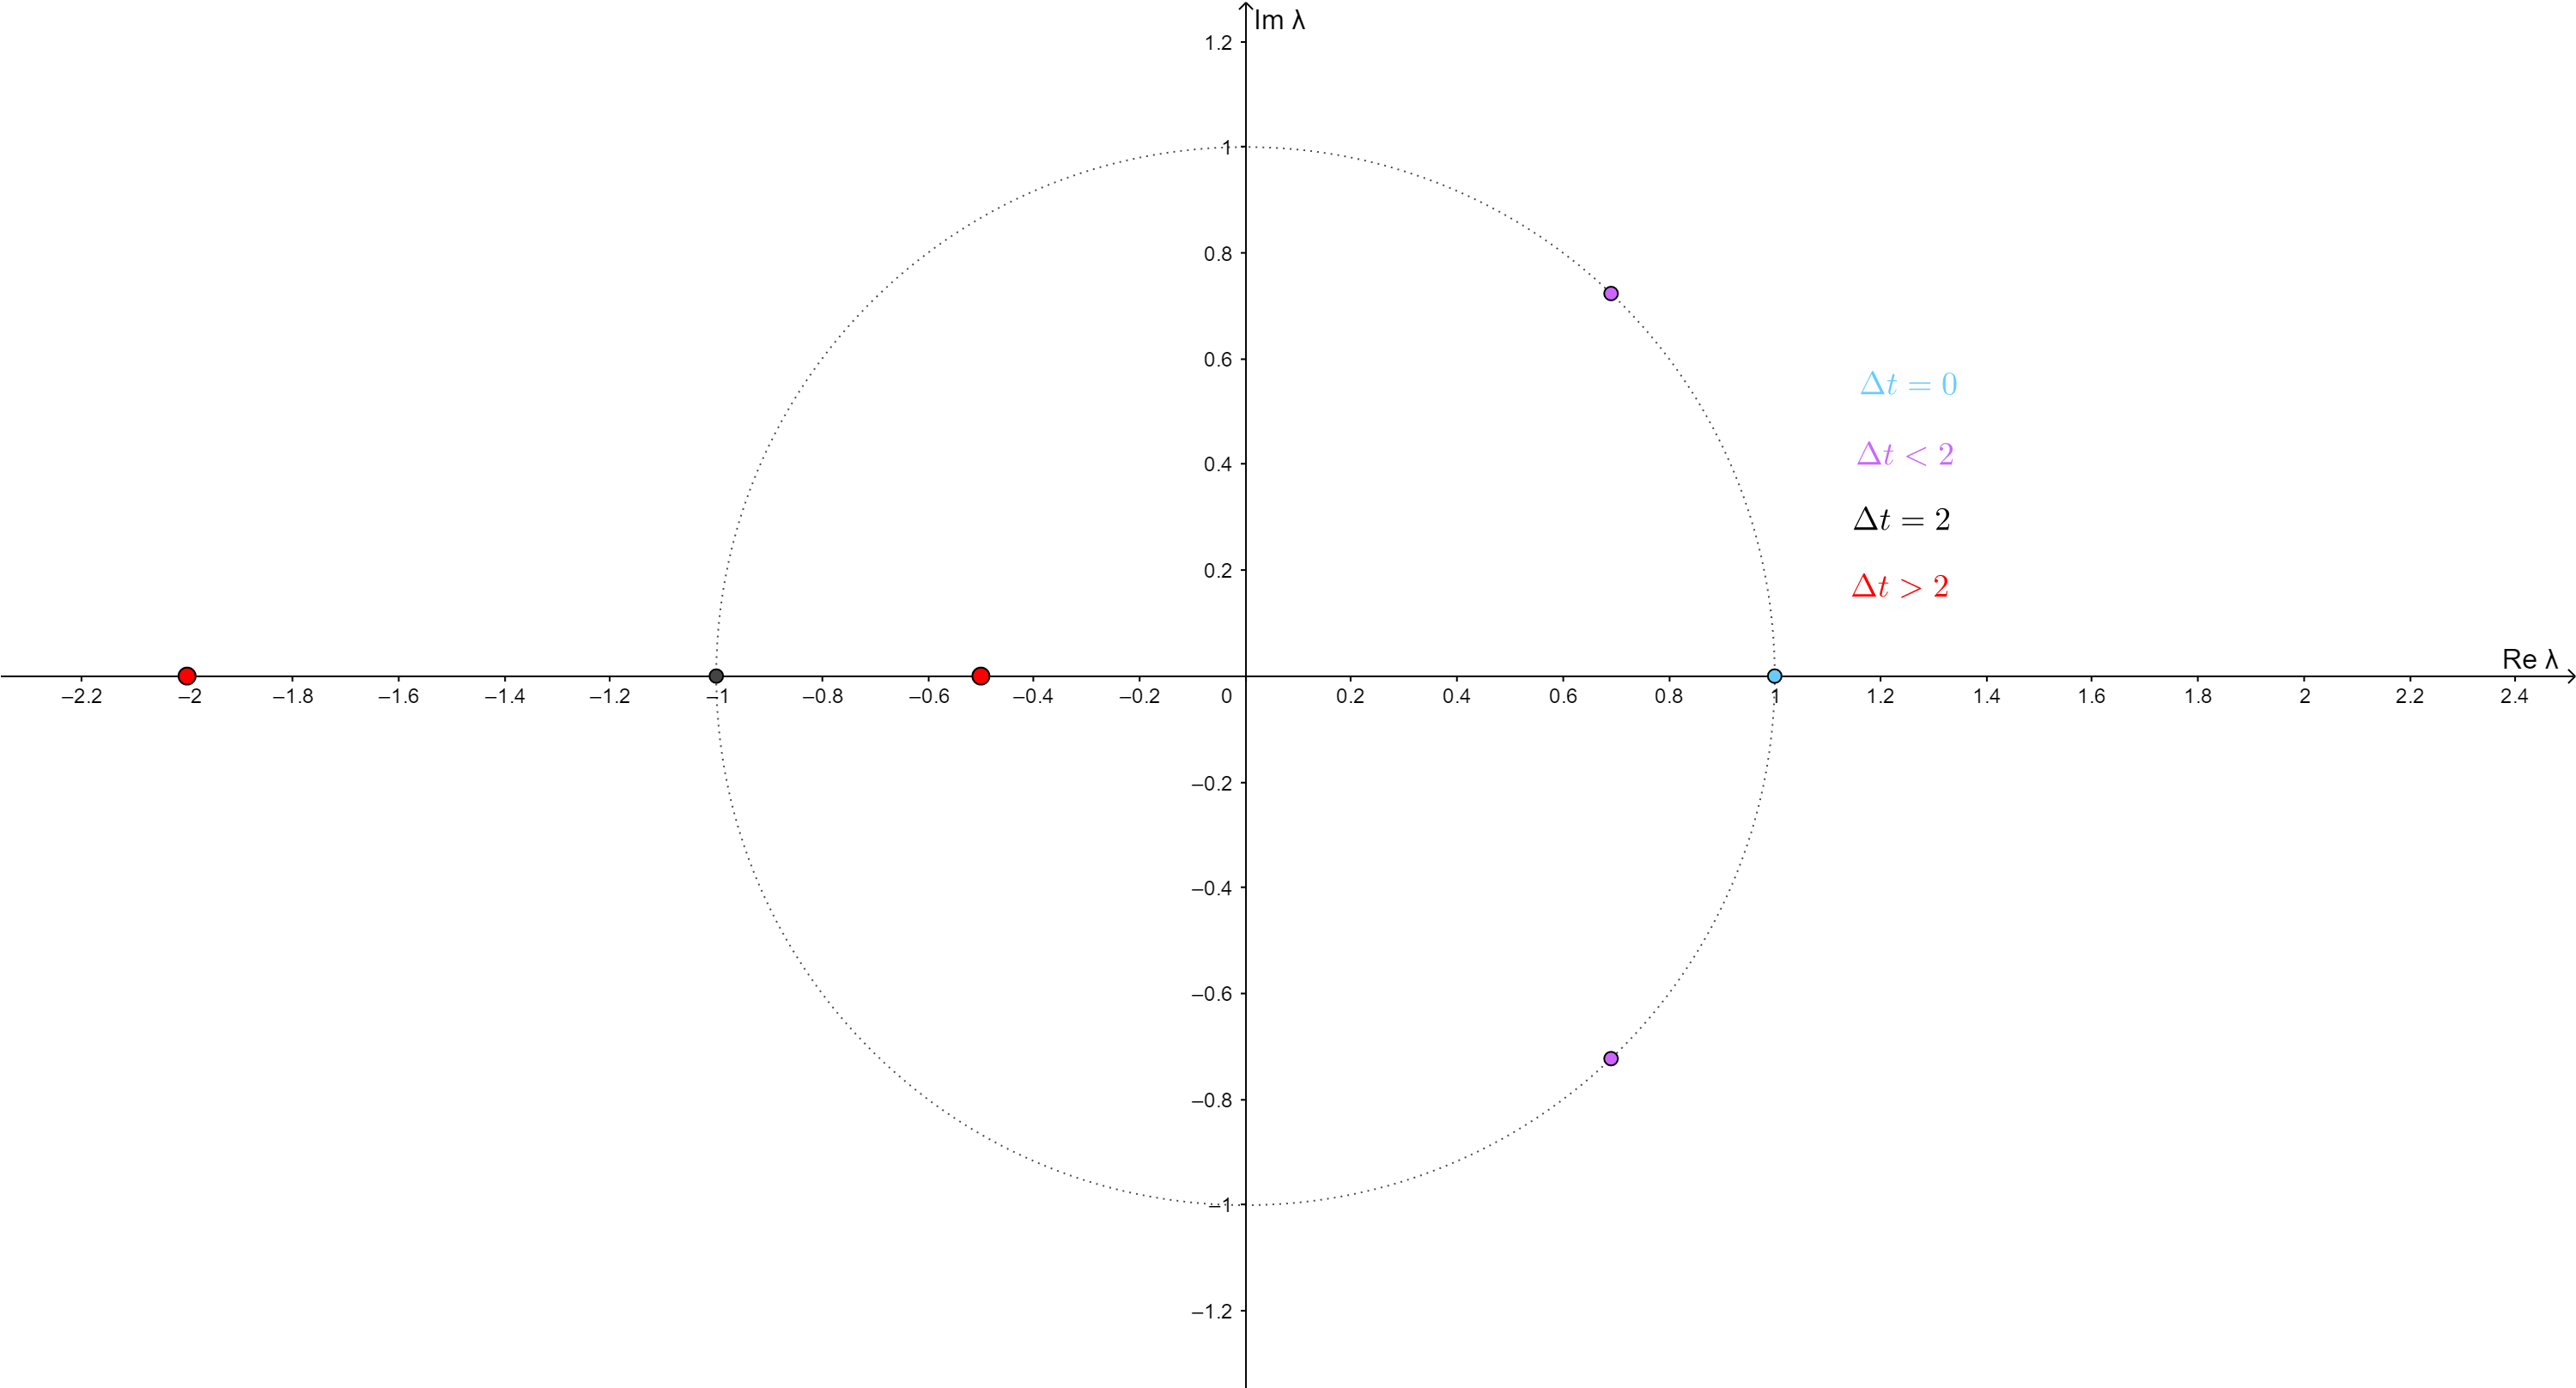
\includegraphics[scale=3.0]{Integrators/images/complexplane.png}
    \caption{Possible eigenvalues of the matrix $A$}
    \label{fig:complexplane}
\end{figure}
In the case where they are complex, their imaginary part is opposite and the real parts are equal.
After n steps:
\begin{equation}
    \begin{pmatrix}
      q' \\
      p'
    \end{pmatrix}
    = A^n
    \begin{pmatrix}
      q \\
      p
    \end{pmatrix}
\end{equation}
Check the behaviour for a large number of time steps ($n\xrightarrow{}\infty$):
\begin{itemize}
    \item if $A^n$ contains some infinite term, then the trajectory will diverge.
    \item if $A^n$ goes to 0, then the trajectory will converge (oscillate around the circular trajectory).
\end{itemize}
The eigenvalues of $A^n$ are equal to the eigenvalues of $A$ raised to the n-th power, therefore:
\begin{itemize}
    \item  $\lambda_1=\lambda_2=-1$: trajectory will oscillate\footnote{$\lambda_1=\lambda_2=1$ is the case when the timestep is equal to zero, therefore the system is not moving}. $$\Delta t = 2$$
    \item $\lambda_1> -1$, $\lambda_2< -1$ or $\lambda_2> -1$, $\lambda_1< -1$: matrix explodes, trajectory diverges. $$\Delta t > 2$$
    \item complex eigenvalues with unitary modulus: trajectory will oscillate.  $$\Delta t < 2$$
\end{itemize}
Threshold for stability of a numerical simulation:
\begin{equation}
    \Delta t < \frac{T}{\pi}
\end{equation}
This is the theoretical limit for the timestep, given the period. The criterion for the timestep is the same for Verlet and Velocity Verlet.
\subsection{Multiple springs}
Let us consider a situation where there are 3 particles with the same mass connected by springs with $k_1 >> k_2$. Let us estimate the maximum time step that should be used. The solution is to take the stiffest spring to impose the limit on the timestep, i.e., that gives the shortest timestep.
In general, this condition is given by the fastest degree of freedom, in other words, by the lightest possible atom with the stiffest spring. This is the way to find the upper bound for our timestep:
computing the period $2\pi \sqrt{\frac{m}{k}}$.
If energy is sufficiently conserved, this means that the timestep is small enough. It is difficult to predict a priori a good value of the timestep because there could be nonlinear potentials.


    \section{The Gran-Canonical ensemble}
Let's now consider a system for which the number of particles is allowed to fluctuate, as if the system were in contact with a larger system at the same temperature, with which it can exchange particles. In order to treat this case, we need to add to the phase space distribution function an extra index accounting for the number of particles N:
\begin{equation}
    \rho(\textbf{q},\textbf{p}) \rightarrow \rho_N(\textbf{q},\textbf{p}).
\end{equation}
A more general definition of Entropy may be written too:
\begin{equation}
        S = -k_B \sum_N \int \frac{d\Gamma_N}{h^{3N}}  \rho_N\ln{\rho_N},\label{S}
\end{equation}
  This corresponds to the most general integration over phase space of the expression $\rho_N\ln{\rho_N}$. $h^{3N}$ is a dimensional factor deriving from quantization of phase space. Being it a constant, we will neglect this factor from now on. Again, due to the maximum entropy principle, an expression for the density $\rho_N$ can be found maximizing entropy with the appropriate constraints:
\begin{itemize}
    \item $\sum_N \int d\Gamma_N  \rho_N = 1 \: \Rightarrow \: \text{normalization} $\\
    \item $\sum_N \int d\Gamma_N  \rho_N H_N = <E> \: \Rightarrow \: \text{mean energy conservation}\\$
    \item $\sum_N \int d\Gamma_N  \rho_N N = <N> \: \Rightarrow \: \text{mean n. of particles conservation}\\$
\end{itemize}
Hence, we're looking for $\rho_N^*$ such that the functional 
\begin{equation}
    \mathcal{F}[\rho_N] = -\sum_N\int d\Gamma_N \rho_N ( \ln{\rho_N} - \lambda + \beta H_N - \beta \mu N)
\end{equation}
is stationary. Imposing: 
\begin{align}
    \partial\mathcal{F}[\rho_N^*] &\equiv \mathcal{F}[\rho_N^*+\delta\rho_N] - \mathcal{F}[\rho_N^*]\\
    &\simeq -\sum_N\int d\Gamma_N \delta\rho_N(\ln{\rho_N^*}+1-\lambda+\beta H_N -\beta \mu N)=0
\end{align}
we get the following expression:
\begin{equation}
\label{eq:rho_micro}
    \rho_N^*=\frac{e^{-\beta(H_N-\mu N)}}{Z_{GC}}\:. 
\end{equation}
An \textit{ad hoc} extra factor $1/N!$ has to be introduced to obtain the correct additive Entropy (see Huang), so that the final result is:
\begin{equation}\label{incriminate} 
    \rho_N^*=\frac{e^{-\beta(H_N-\mu N)}}{N! Z_{GC}},\hspace{0.5 cm} \text{with} \: Z_{GC}= \sum_N\int d\Gamma_N \frac{e^{-\beta(H_N-\mu N)}}{N!}.
\end{equation}
The new Lagrange multiplier we have introduced, $\mu$, is called \textit{chemical potential}. We will later give an interpretation for it.\\

\textit{\textbf{Comment:} I believe Micheletti was imprecise here. In eq.\ref{incriminate} the factor $1/N!$ should be present in the expression for $Z$ but not in the one for $\rho$. Actually, if both expressions contained it, we would be multiplying $\rho$ for a $N!/N!=1$ factor and eq.\ref{S} would remain unchanged. The correct interpretation is the following: being atoms quantum mechanically indistinguishable, any permutation of the atoms indexes does not produce a new state of the system. Then the factor $1/N!$ accounts for the fact that an infinitesimal volume $dpdq$ in phase space corresponds to $dpdq/N!$ different micro-states only. In conclusion, when taking averages of functions $f(p,q)$ over the possible micro-states of the system, we should write integrals as:
\begin{equation}
    <f> = \sum_N \int \frac{d\Gamma_N}{N!h^{3N}}  \rho_N f(q,p).
\end{equation}
This explains why $1/N!$ is only present in the expression for $Z$. Also, computing entropy like this all factors $1/N!$ simplify apart from the one inside the logarithm, so that we obtain the correctly rescaled expression.
}\\

As an example, we can compute the Gran-Canonical partition function $Z_{GC}$ for an ideal gas:
\begin{equation}
    \begin{split}
    Z_{GC} &= \sum_N \frac{1}{N!}\int d\Gamma_N e^{-\beta(H_N-\mu N)}\\
    &=\sum_N \frac{e^{\beta \mu N}}{N!}\int d\Gamma_N e^{-\beta H_N}\\
    &=\sum_N \frac{e^{\beta \mu N}}{N!}V^N\biggl( \frac{2\pi m}{\beta}\biggr)^{3N/2}\\
    &=\sum_N \frac{x^N}{N!}=e^x, \hspace{0.5 cm} \text{with} \:x=e^{\beta \mu}V \biggl(\frac{2\pi m}{\beta}\biggr)^{3/2}.
    \end{split}
\end{equation}
We have used the expression \ref{eq:zcannone} for the Canonical partition function computed in the previous section. We call the factor $z=e^{\beta \mu}$ \textit{fugacity}. The mean number of particles $<N>$ can be computed too. Being $Z_{GC}$ a cumulant generating function, 
\begin{equation}
    <N>=\frac{\partial ln Z_{GC}}{\partial (\beta \mu)}
    =e^{\beta \mu}V \biggl(\frac{2\pi     m}{\beta}\biggr)^{3/2}. \label{eq.N}
\end{equation}
Consequently:
\begin{equation}
   \begin{split}
    & e^{-\beta \mu}=\frac{V}{<N>}\biggl(\frac{2\pi m}{\beta}\biggr)^{3/2} \\
    & \mu=-K_B T ln \biggl[\frac{V}{<N>}\biggl(\frac{2\pi m}{\beta}\biggr)^{3/2} \biggr].
    \end{split}
\end{equation}
The equation we have obtained for $\mu$ tells us something important about its physical interpretation. Recalling the equation for the \textit{free energy} for a canonical ensemble in the case of an ideal gas,
\begin{equation}
    \begin{split}
    F_{CAN}&=-k_B T \ln{Z_{CAN}}\\
    &=-k_B T ln\biggl[ \frac{V^N}{N!}\left(\frac{2\pi m}{\beta} \right)^{3N/2}\biggr]\\
    &=-k_B T \biggl[N\ln{V}-ln(N!)+\frac{3N}{2}\ln{\left(\frac{2\pi m}{\beta} \right)}\biggr]\\
    &\simeq -k_B T \biggl[N\ln{V}-(NlnN-N)+\frac{3N}{2}\ln{\left(\frac{2\pi m}{\beta} \right)}\biggr],\\
    \end{split}
\end{equation}
where we have used Stirling's approximation, we have that:
\begin{equation}
   \frac{\partial F_{CAN}}{\partial N}=-K_B T ln \biggl[\frac{V}{N}\biggl(\frac{2\pi m}{\beta}\biggr)^{3/2} \biggr]=\mu.
\end{equation}
In conclusion, $\mu$ corresponds to the difference in \textit{free energy} due to variations of the number of particles the system is composed of.

\subsection{Equilibrium condition for chemical reactions}
The \textit{chemical potential} $\mu$ turns out to be very useful in some chemistry problems. Let's consider a generic chemical reaction involving n reactants and m products:
\begin{equation}
    \nu_1 x_1 + ... + \nu_n x_n \rightleftharpoons \nu_{n+1} x_{n+1} + ... + \nu_{n+m} x_{n+m}
\end{equation}
Clearly, when elements react, the number of molecules $N_i$ of element i varies: $N_i \rightarrow N_i+\delta N_i$. This makes the system we're studying a Gran-Canonical one. On the other hand, starting from equilibrium, the ratio $\delta N_i/\nu_i$ between the variation of the number of molecules of element i and its stoichiometric coefficient must be constant and equal for all i's. Also, if the system keeps at equilibrium the \textit{free energy} F must be minimal. Then:
\begin{equation}
    \begin{split}
    \partial F &= F(N_1+\delta N_1,...,N_{n+m}+\delta N_{n+m})-F(N_1,...,N_{n+m})\\
    &=\frac{\partial F}{\partial N_1}\delta N_1+...+\frac{\partial F}{\partial N_{n+m}}\delta N_{n+m}\\
    &=\mu_1 \delta N_1+...+\mu_{n+m} \delta N_{n+m}=0.
    \end{split}
\end{equation}
Knowing $\delta N_i/\nu_i= const=\delta N$, with $\delta N$ arbitrary, we get to the equilibrium condition:
\begin{equation}
    \sum_i \mu_i \nu_i=0.
\end{equation}
Notice that, for convention, stoichiometric coefficients $\nu_i$ are positive for reactants and negative for products. This same condition may be written in terms of the fugacity $z$ as:
\begin{equation}
    e^{\beta\sum_i \mu_i \nu_i}=\prod_i (z_i)^{\nu_i}=1.\label{eq.fugacity}
\end{equation}
From eq.\ref{eq.N}:
\begin{equation}
    z=\bigl[ v \bigl( \frac{2\pi m}{\beta}\bigr)^{3/2}\bigr]^{-1}, 
\end{equation}
where $v=\frac{V}{N}$ is the concentration of the $i_{th}$ element. Then eq.\ref{eq.fugacity} tells us:
\begin{equation}
    \prod_i v_i^{\nu_i}\sim\prod_i (m^{\nu_i})^{-3/2}.  
\end{equation}
This is known as the law of mass action, stating that the the quantity $\prod_i v_i^{\nu_i}$ is a constant for reactions at equilibrium, namely the \textit{equilibrium constant}.  
\chapter{Monte Carlo}
    \section{Introduction}
In molecular dynamics, a thermostat is an algorithm built with the purpose of generating samples from a statistical ensemble at constant temperature $T$.
At this point, we know that the typical choice among the statistical ensembles, when simulating a real physical system, is the Canonical one, which allows fluctuations of the total energy under the constraint that its average remains constant over time.
Therefore, our aim will be to build thermostats which sample configurations drawn from the Canonical ensemble. 

Before entering in the implementation of these algorithms, let's recall some of the main features of the ensemble we are interested in.

\subsection{Recap of the Canonical ensemble}
The probability distribution related to the Canonical ensemble, as defined in Chapter 1 (1.36), is given by
\begin{equation}
     P(x)=\frac{e^{-\beta H(x)}}{Z}
\end{equation}
with 
\begin{equation}
     Z=\int_ {}^{} e^{-\beta H(x)}dx
\label{zetafunc}
\end{equation} 

\par Is important to remember that here $x$ represents a vector that contains the position and momenta of all the particles of the system, so the integral (5.2) is taken over all the points composing the phase space of our system. 

As we have already seen, this formulation allows us to compute the average of a generic observable $A(x)$ as
\begin{equation}
     \langle A \rangle =\int_ {}^{} P(x)A(x)dx,
\end{equation}

and, as a consequence, its variation with respect to the temperature as
\begin{equation}
    \frac{\partial \langle A \rangle}{\partial T}=-\frac{1}{k_B T^2} (-\langle HA \rangle+\langle H \rangle\langle A\rangle). 
\end{equation}

Some relevant examples are the derivatives of the average values of:
\begin{itemize}
    \item The total energy $H$
    \begin{equation}
      \frac{\partial \langle H \rangle}{\partial T}=\frac{1}{k_B T^2} (\langle H^2\rangle-\langle H\rangle^2)=\frac{1}{k_B T^2}\sigma_H^2
    \end{equation} 
    which is proportional to the variance of $H$ (i.e. the amplitude of its fluctuations) and which can be physically interpreted as the amount of energy needed in order for the temperature to increase by 1 degree, i.e. the Heat capacity; 
    \item The potential energy $U$
    \begin{equation}
        \frac{\partial \langle U \rangle}{\partial T}=\frac{1}{k_B T^2} (\langle U^2 \rangle -\langle U \rangle^2)=\frac{1}{k_B T^2}\sigma_U^2 ;
    \end{equation}
    \item the kinetic energy $K$
    \begin{equation}
        \frac{\partial \langle K \rangle}{\partial T}=\frac{1}{k_B T^2} (\langle K^2\rangle-\langle K \rangle^2)=\frac{1}{k_B T^2}\sigma_K^2 .
    \end{equation}
\end{itemize}

In particular, the last two results are obtained exploiting the feature of the Hamiltonian of the majority of the systems we are interested in, built as the sum of a kinetic contribution \begin{math} K(p)=\sum_{i=1}^{N_a} \frac{{p_i}^2}{2m_i} \end{math}, which depends only on the momenta $p_i$ of the particles, and a potential contribution $U(q)$, specific of the system, which depends only on the positions $q_i$. 

This composition of the Hamiltonian makes the probability distribution $P(x=p,q)$ factorizable into two separate parts: \begin{math}P_K(p) \propto e^{-\beta \sum_{i=1}^{N_a} \frac{p_i^2}{2m_i}} \end{math} (which is a gaussian) and $P_U(q)$.

Then, from  $P_K(p)$ we can obtain the probability distribution of the kinetic energies $P_K(K)$, which is not a gaussian (because as $K<0$, $P_K$ is identically equal to $0$), but a Gamma distribution
\begin{equation}
    P_K(K) \propto K^{N_F/2 -1}e^{-\beta K}
\end{equation}
where $N_F=3N_a$ is the number of degrees of freedom, with average
\begin{equation}
    <K>=\frac{3}{2} N_a k_B T \implies \frac{\partial <K>}{\partial T}=\frac{3}{2} N_a k_B
\end{equation}

and width (from (5.7) and (5.8))
\begin{equation}
    \sigma_K=\sqrt{k_B T^2 \frac{\partial <K>}{\partial T}}=\sqrt{\frac{3}{2} N_a k_B^2 T^2}= \sqrt{<K>^2 \frac{2}{3 N_a}}.
\end{equation}
In particular, the factor $K^{N_F/2 -1}$ is in some way related to the density of state: this explains why negative kinetic energies are not allowed ($P_K(K<0)=0$) and why, without the compensation of the Boltzmann factor \begin{math} e^{-\beta K} \end{math}, high kinetic energies would be more likely.
A qualitative description of the behaviour of $P_K(K)$ can be seen in Figure \ref{fig:kinetic distribution}

\begin{figure}
    \centering
    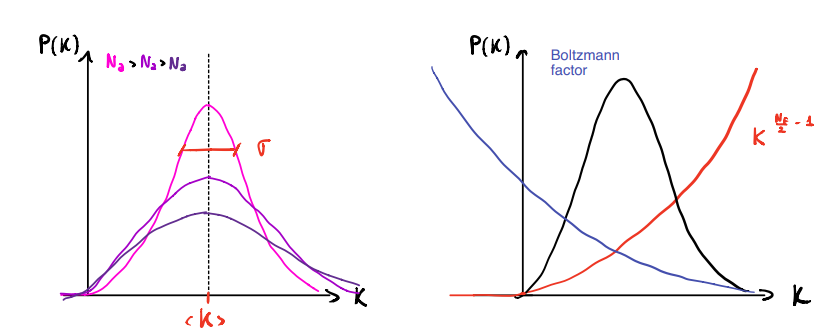
\includegraphics[width=0.7\textwidth]{Thermostats/images/kinetic distribution.PNG}
    \caption{On the left: qualitative behaviour of the Gamma distribution $P_K(K)$ at different values of $N_a$, always centered in the same value in order to compare visually the different shapes. On the right: qualitative behaviour of the two factors that compose $P_K(K)$, whose coexistence leads to the typical shape of the Gamma distribution.}
    \label{fig:kinetic distribution}
\end{figure}

\section{Algorithms}

As mentioned in the Introduction, the two main properties of the thermostats we want to implement are:
\begin{itemize}
    \item Equilibration of the system to a target value of the temperature $\bar T$, that, after an early transient, have to remain constant;
    \item Production of configurations drawn from the Canonical ensemble.
\end{itemize}

First of all, we have seen, as one of the main results of the theoretical description of the Canonical ensemble, that \begin{math} <K> \propto T \end{math}. 
Therefore, we can think about controlling the value of the temperature through the control of the kinetic energy $K(p)$, which will have to reach the target value $\bar K \propto \bar T$. This control on $K(p)$ can be realized imposing proper variations of $K(p)$ itself, in such a way that $<K>= \bar K$. 

But this will not be sufficient in order to satisfy the second request: in fact, in order for our simulation to produce canonical configurations, we need also the fluctuations on $K(p)$ to be coherent with the canonical distribution, and so equal to its variance $\sigma_K^2$.

As a consequence of these requirements, the main idea to implement thermostats is by choosing a rule for the variation of $K(p)$, and evolving the system through a modified version of Hamilton equations, which will determine variations of potential energy $U(q)$ in such a way that the ones of $K(p)$ are balanced, and so that the total energy is approximately conserved.


\subsection{Trial and error}

The first attempt, which can not be called an actual algorithm, but is useful to introduce us to the logic underlying thermostats, is the "Trial and error". 
It exploits the behaviour of the simulation to set the proper value of the initialization $K_0$ which, after a transient, will lead to the target value \begin{math} \bar K \end{math} (and so to the target value \begin{math} \bar T \end{math}).

At first, in fact, we could try initializating the kinetic energy at its target value. Unfortunately, starting the simulation we would see that $K$ doesn't remain constant at $\bar K$, but equilibrates to a different value.

So, we could think of starting a new simulation from a different $K_0$, shifted from the previous by the difference between $\bar K$ and the previous equilibration value.
Typically, the optimal result can not be reached in a unique attempt, but after various iterations, which can be stopped when the difference between $\bar K$ and the new equilibration value of $K$ is small enough.

\begin{figure}
    \centering
    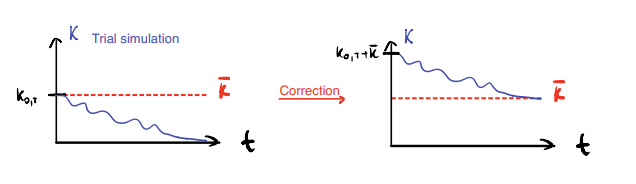
\includegraphics[width=0.7\textwidth]{Thermostats/images/Trial and error.PNG}
    \caption{The first image represent the Trial simulation, where the kinetic energy is initialized to its target value. The second represent the correct simulation, where the initialization is set to that value from which, after the equilibration, the kinetic energy reaches the target value.}
    \label{fig:trial and error}
\end{figure}

In Figure \ref{fig:trial and error} we see how this procedure would look if a unique attempt would be sufficient.

Unfortunately, as we can imagine looking at the triviality of this algorithm, this is not a suitable choice for implementing a thermostat.

\subsection{Velocity rescaling}
The Velocity rescaling algorithm is based on the following idea:
\begin{itemize}
    \item Given an initial configuration of the system, we run a number \textit {stride} of steps using a Hamilton equations integrator, like, for example, Velocity Verlet;
    \item We check the istantaneous value of $K$ and we change it rescaling it by a factor that makes it equal to the target value $\bar K=\frac{3}{2}N_a K_B \bar T$.
\end{itemize}

A pseudocode representing these operations would be:
\begin{algorithm}[H]\label{velocity_rescaling}
			\caption{Velocity rescaling algorithm}
			\begin{algorithmic}[1]
				\For{$i step\; inrange (nsteps)$}
    				\State $p+=f*\Delta t/2$
    				\State $q+=p*\Delta t/m$
    				\State $p+=f*\Delta t/2$
    				\If{$i step\%stride==0$}
    				    \State $K= \frac{\sum_{i}{p_i^2}}{{2m_i}}$
    				    \State $p* = \sqrt{\frac{\Bar{K}}{K}}$
    				\EndIf
				\EndFor
			\end{algorithmic}
		\end{algorithm}

\begin{figure}
    \centering
    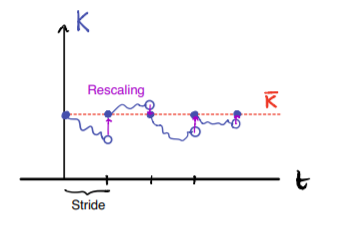
\includegraphics[width=0.7\textwidth]{Thermostats/images/velocity rescaling.PNG}
    \caption{Example of a trajectory $K(t)$ produced using the Velocity rescaling thermostat.}
    \label{fig:velocity rescaling}
\end{figure}		

As we can see, in this case the change in the kinetic energy is made on its total value, and not on the specific values $K_i$ of the single particles: this feature defines the so called \textit {Global thermostats}.

Although, as also qualitatively represented in Figure \ref{fig:velocity rescaling}, this algorithm works well in the equilibration to the target value $\bar K$, reached in a time interval $\propto {\textit {stride}}$, this is not an optimal choice for two main reasons: first of all, the distribution we are sampling from is unknown, and certainly it is not the canonical since the fluctuations of $K$ are not the proper ones (see Figure \ref{fig:fluctuations}); then, the trajectory is discontinuous, and this does not allow us to convert the algorithm into a differential equation.

\begin{figure}
    \centering
    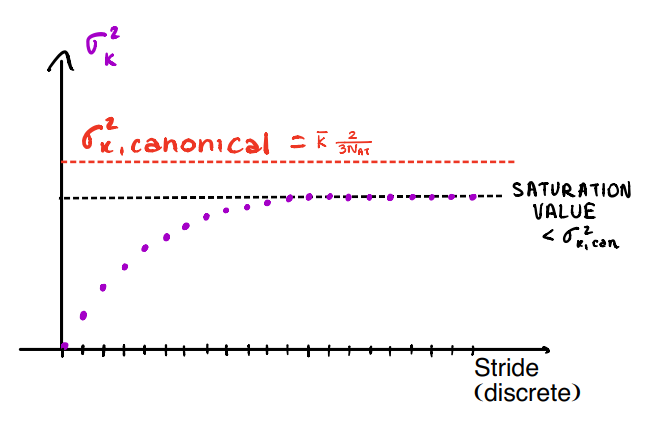
\includegraphics[width=0.7\textwidth]{Thermostats/images/fluctuations.PNG}
    \caption{Behaviour of $\sigma_K^2$ as a function of \textit {stride}. If \textit {stride} is small, the trajectory is smoother and $<K>=\bar K$, but the fluctuations are too small. If \textit{stride} is too big, the fluctuations will reach a saturation value smaller than the correct one, and also $K$ doesn't reach the target: in fact, this choice would basically correspond to evolving the system according to Velocity Verlet, which guarantees the conservation of the total energy and then produces configurations drawn from the Microcanonical distribution. }
    \label{fig:fluctuations}
\end{figure}

\subsection{Berendsen thermostat}
The problem of discontinuity in Velocity rescaling algorithm is soon solved by the Berendsen thermostat, which can be interpreted as its "continuous version".

It is based on the idea of modifying $K$ at each step, rescaling it by a properly weighted sum of the current value and the target value.

In practice, this operation would consist into the multiplication of the current value of the momentum $p$ by a factor
\begin{equation}
    F={\sqrt{\frac{c_1K+c_2 \bar K}{K}}}.
\end{equation}

In particular, the choice of the weights ${c_1}$ and ${c_2}$ has to guarantee the following properties:
\begin{itemize}
    \item $c_1+c_2=1$
    since, when $K=\bar K$, the factor F must be equal to 1, because the target value has been reached, and then we do not have to modify the current value;
    \item the limit $c_1 \rightarrow 1$ ( $\implies c_2 \rightarrow 0$), which represents the absence of the thermostat (since there are no corrections to the current values $p$) should coincide with the limit case of $\textit{stride}=\tau \rightarrow \infty$ in Velocity rescaling;
    \item the limit $c_2 \rightarrow 1$ ($\implies c_1 \rightarrow 0$), which basically respresents the application of Velocity rescaling at each step, should coincide with the limit case of $\textit{stride}=\tau \rightarrow 0$.
\end{itemize}

A choice which guarantees the latter requests is:
\begin{equation}
   c_1=e^{-{\frac{\Delta t}{\tau}}} ;\quad
      c_2=1-c_1=1-e^{-{\frac{\Delta t}{\tau}}}
\end{equation}

At this point, we can try converting the algorithm into a differential equation:
\begin{multline*}
    K_{new}={\frac{e^{-{\frac{\Delta t}{\tau}}}K+\left(1-e^{-{\frac{\Delta t}{\tau}}}\right) \bar K}{K}}K \\ 
    \implies \Delta K=K_{new}-K=e^{-{\frac{\Delta t}{\tau}}}K + (1-e^{-{\frac{\Delta t}{\tau}}}) \bar K - K \\
    = (1-e^{-{\frac{\Delta t}{\tau}}} )(\bar K -K) 
\end{multline*}

Then, performing the infinitesimal limit:
\begin{equation*}
    \lim_{{\Delta t}\to 0} \Delta K = (1-1+\frac{\Delta t}{\tau} + \textit{h.o.t})(\bar K-K)=\frac{\Delta t}{\tau}(\bar K-K)
\end{equation*}

\begin{equation}
    \implies dK=dt \frac{(\bar K-K)}{\tau}
\end{equation}

that is actually a differential equation. This means its solution, i.e. $K(t)$, is continuous, and then we can say that the issue we had with Velocity rescaling is solved.

Another advantage with respect to Velocity rescaling is that now we have a control parameter $\tau$, which, differently from \textit{stride}, has a physical interpretation:
it is the relaxation time of the system, and gives a qualitative measure of the thermal inertia of it, since the greater is $\tau$, the more difficult will be to change $K$, namely $T$.

Moreover, as a smoother version of Velocity rescaling, Berendsen's is itself a global thermostat.

So, in conclusion, one of the main advantages of using this algorithm is that the trajectories it produces are continuous, but it is not the only one. In fact, according to the huge number of citations of the original paper by Berendsen (1984), it is probably the most used thermostat, and this is due to a series of properties: it empirically equilibrates well; it is easy to understand; it is efficient. Regarding the efficiency, this is what actually makes people prefer this algorithm to more exact ones like, for example, Hybrid Montecarlo: indeed, the approximation makes Berendsen thermostat quicker in simulating very large systems, for  which a more accurate algorithm would take a too long time.

However, this algorithm does not sample configurations from the canonical distribution. In fact, even if balance is satisfied, because a stationary distribution can be reached, this is not the canonical one, and this is due to the fact that $K$ does not respect the proper fluctuations. Detailed balance is instead not guaranteed, because $K$ is forced to reach $\bar K$ and a time-reversed trajectory is not even possible.




    \section{Maximum entropy principle and microcanonical ensemble}
As before, consider a system divided in two compartments with energies $E_1$ and $E_2$. The two subsystems can exchange energy, but the sum $E_1+E_2 = E$ is fixed. We have already demonstrated that the phase space of the system at the equilibrium is given by 
\begin{equation}
    \Gamma_{1+2}(E) = \Gamma_1(E_1^*)\,\Gamma_2(E-E_1^*),
\end{equation}
where $E_1^*$ is the energy that maximizes $\Gamma_{1+2}$. This relation is clearer if one thinks of $\Gamma_i$ as the degeneracy of a state with an energy $E_i$. The equilibrium condition then becomes
\begin{equation}
    \frac{\partial \Gamma_{1+2}}{\partial E_1}\bigg|_{E_1^*} = \frac{\partial \Gamma_1(E_1)}{\partial E_1} \Gamma_2(E - E_1) + \Gamma_1(E_1)\frac{\partial \Gamma_2(E - E_1)}{\partial E_1} = 0.
\end{equation}
Since we have the constraint $E_2 = E-E_1$, we can take the derivative of $\Gamma_2$ with respect to $E_2$, changing its sign. Ordering the terms and multiplying by the Boltzmann constant $k_B$ we obtain
\begin{equation}
    \frac{k_B}{\Gamma_1} \frac{\partial \Gamma_1}{\partial E_1} = \frac{k_B}{\Gamma_2} \frac{\partial \Gamma_2}{\partial E_2} \: \Longrightarrow \:
    k_B \frac{\partial (\ln{\Gamma_1})}{\partial E_1} = k_B \frac{\partial (\ln{\Gamma_2})}{\partial E_2}
\end{equation}
and $k_B\ln{\Gamma}$ was our definition of entropy $S$. So the equilibrium condition is 
\begin{equation}
    \frac{\partial S_1}{\partial E_1} = \frac{\partial S_2}{\partial E_2}
\end{equation}
which is equivalent to having the same temperature. \\ \\

Entropy is an observable, so its expected value can be written as $S = \int d\Gamma \rho f(q,p)$ for a certain function $f$ of positions and momenta. From an analogy with probability theory and Shannon entropy, entropy turns out to be
\begin{equation}
    S = -\int d\Gamma \rho \ln{\rho}.
\end{equation}
which is also equal to $S=\ln{\Gamma}$ (for $k_B=1$).
We don't give a formal proof of this statement, but we show that it gives correct results in two particular limit cases:
\begin{itemize}
    \item case 1: $n$ energy levels, with $p_1 = 1$ and $p_{i\neq 1} = 0 \: \Rightarrow \: S=0$. \\
    \item case 2: $p_i = 1/n$ for all $i \: \Rightarrow \: S= -\frac{1}{n}\ln(\frac{1}{n})^n = \ln{n}$.
\end{itemize}
The maximum entropy principle states that a system in equilibrium tends to maximize entropy, given the constraints, for every probability density $\rho$. For the microcanonical ensemble, we consider the following constraints for $\rho$:
\begin{gather}
    \int d\Gamma \rho = 1 \: \Rightarrow \: \text{normalization} \\
    \rho(\mathbf{q},\mathbf{p}) = 0 \: \text{if} \: H(\mathbf{q},\mathbf{p}) \not\in (E,E+\Delta).
\end{gather}
For $k_B=1$, $S = -\int d\Gamma \rho \ln{\rho}$ and introducing the Lagrange multiplier $\lambda$ we can construct the functional
\begin{equation}
    \mathcal{F}[\rho] = -\int d\Gamma (\rho \ln{\rho} - \lambda\rho)
\end{equation}
and our goal is to find $\rho^*$ that makes it stationary. More explicitly, we want the functional differential
\begin{equation}
    \partial\mathcal{F}[\rho^*] \equiv \mathcal{F}[\rho^*+\delta\rho] - \mathcal{F}[\rho^*]
\end{equation}
with no linear terms in $\delta\rho$. Then we get
\begin{align}
\label{eq:rho_micro}
    \partial\mathcal{F}[\rho^*] &= -\int d\Gamma [(\rho^*+\delta\rho)\ln(\rho^*+\delta\rho) - \lambda(\rho^*+\delta\rho)] + \int d\Gamma (\rho^*\ln\rho^* - \lambda\rho^*) \nonumber \\
    &= -\int d\Gamma (\delta\rho\ln{\rho^*}+\delta\rho-\lambda\,\delta\rho) + h.o.t. \nonumber \\
    &= -\int d\Gamma \delta\rho \,(\ln{\rho^*}+1-\lambda) = 0
\end{align}
where in the second line we have used the fact that 
\begin{equation}
    \ln(\rho^*+\delta\rho) \simeq \ln{\rho^*} + \frac{\delta\rho}{\rho^*} + h.o.t.
\end{equation}
Since eq. (\ref{eq:rho_micro}) has to hold for every $\delta\rho$, the integrand must be null, i.e.
\begin{equation}
    \ln{\rho^*}(\mathbf{q},\mathbf{p}) = \lambda-1
\end{equation}
that does not depend on $\mathbf{q}$ and $\mathbf{p}$, so we obtain a uniform \textit{a priori} probability. This is due to the fact that we had no constraints, except for the normalization of the probability density. We can repeat the same calculation adding the constraint 
\begin{equation}
    \int d\Gamma \rho\,H = \bar{E}
\end{equation}
that corresponds to the canonical ensemble.




    %by Elena C. WORK IN PROGRESS
\subsection{Leapfrog Algorithm}
The Velocity Verlet algorithm shown previously (Algorithm \ref{alg:velocity_verlet}) can be modified to reduce the computational cost.\\ In particular, compute a force is quite expensive: computing the force twice will require twice the simulation time. One solution to reduce the computational cost is to merge the momenta shifts together (using the same value of the force): this leads to a slightly faster simulation, but on the other side this kills the possibility of printing the values of p and q at the same time (access to the phase space). This solution is called \textbf{Leapfrog algorithm}.\\
\begin{algorithm}[H]
			\caption{Leapfrog algorithm}
			\label{alg:leapfrog}
			\begin{algorithmic}[1]
			    \State $p=p+f*\Delta t/2$	\For{$i=1,...,nsteps$}
    			\State	$q=q+p/m \Delta t$
                 \State	$f=force(q)$
    			\State	$p=p+f*\Delta t$
				\EndFor
			\end{algorithmic}
		\end{algorithm}
Momentum and position are moved in an alternate way: at the end of a cycle, we do not find the values of the positions and momenta at the same timestep, they are found at a difference of half timestep. Slightly faster than Velocity Verlet, not very significant. 
\begin{figure}[H]
    \centering
    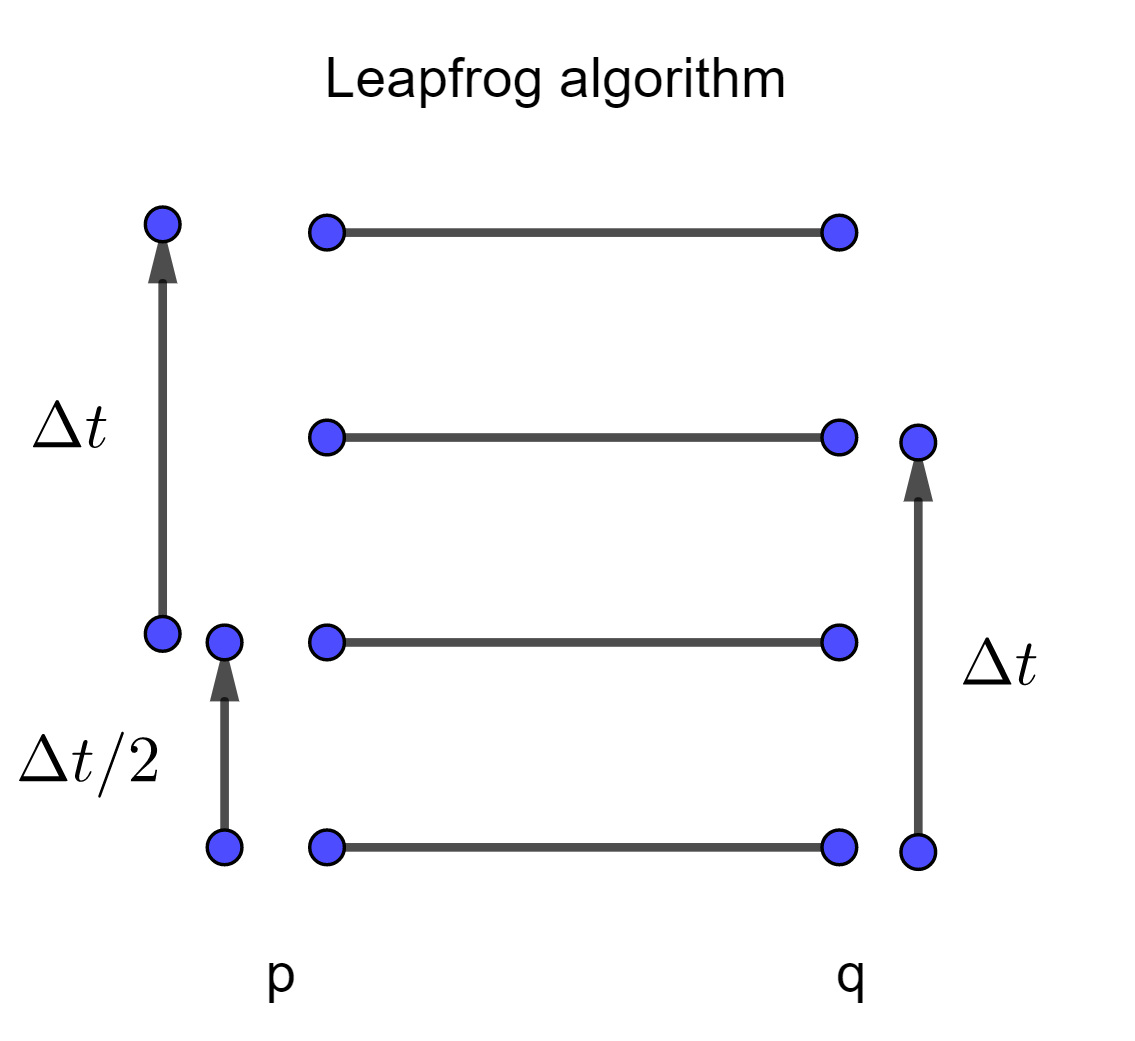
\includegraphics[width=50mm,scale=0.5]{Integrators/images/leapfrog.png}
    \caption{Scheme of the leapfrog algorithm}
    \label{fig:leapfrog}
\end{figure}
\subsection{Position Verlet}
Another alternative to the Velocity Verlet algorithm it is the so-called \textbf{Position Verlet algorithm}.
\begin{algorithm}[H]
			\caption{Position Verlet}
			\label{alg:position_verlet}
			\begin{algorithmic}[1]
        	\For{$i=1,...,nsteps$}
			\State	$q=q+p/m* \Delta t/2$
			\State	$f=force(q)$
			\State	$p=p+f*\Delta t$
			\State	$q=q+p/m* \Delta t/2$
				\EndFor
			\end{algorithmic}
		\end{algorithm}
This algorithm is the swapped version of Velocity Verlet, where the free particle is evolved for half timestep, then the infinite mass system is evolved for one timestep, then the free particle again for half timestep. 
\begin{itemize}
    \item \textbf{Advantages:} the force is computed only once, which is computationally advantageous (only one update of the momentum).
    \item \textbf{Disadvantages:} I cannot print the total energy. Potential energy needs to be computed with a similar procedure to the computation of forces (very expensive). Therefore, it is more convenient to compute forces and energies at the same time, but it is not possible with Position Verlet. Moreover, this algorithm is less used than Velocity Verlet, which is the simplest one.
\end{itemize}

\subsection{Other considerations on the Velocity Verlet algorithm}
Let us recall the Velocity Verlet algorithm:
    \begin{equation}\label{velocityverlet}
            \begin{cases}
                q(t+\Delta t)= q(t)+\frac{p(t)}{m}\Delta t+ \frac{f(t)}{m}\frac{\Delta t^2}{2}\\
                p(t+\Delta t)= p(t)+\frac{f(t)}{2}\Delta t+ \frac{f(t+\Delta t)}{2}\Delta t
            \end{cases}
            \end{equation}
Let's prove that the trajectories obtained with Velocity Verlet are equivalent to those obtained with Verlet algorithm. Trajectories are exactly time reversible, which means that we are allowed to compute $q(t-\Delta t)$ changing the sign of $\Delta t$ in the first equation \ref{velocityverlet}:
\begin{equation}\label{t-dt}
q(t-\Delta t)= q(t)-\frac{p(t)}{m}\Delta t+ \frac{f(t)}{m}\frac{\Delta t^2}{2}
\end{equation}
Let us sum $q(t-\Delta t)$ and $q(t+\Delta t)$ (first eq. \ref{velocityverlet} and eq. \ref{t-dt}):
\begin{equation*}
    q(t-\Delta t)+q(t+\Delta t)=2q(t)+\frac{f(t)}{m}\Delta t^2
\end{equation*}
This is consistent because equation \ref{velocityverlet} for the positions resembles a Taylor expansion of q.  The introduction of operator formalism is significant only for the sake of studying the evolution of momenta, while the evolution of positions is equivalent to the one obtained with the Verlet algorithm. 
In fact, the same trajectory results from the application of Verlet and Velocity Verlet algorithms.\\
Differences between the two algorithms are found by the fact that the Verlet algorithm considers differences between positions (current position $q(t_0)$ minus previous position $q(t_0-\Delta t$)): this leads to large round-off errors. Meanwhile, this problem is not present in Velocity Verlet, which is more numerically stable. Moreover, Velocity Verlet already includes a definition of the velocity, not present in Verlet algorithm: in the former case it is possible to compute the total energy and check if it is conserved.
We recall the properties of Velocity Verlet already discussed in section \ref{chapt:properites_vel_verlet}:
\begin{itemize}
\item \textbf{Trajectory is time reversible.}
\item \textbf{Volume in phase space is conserved.}
\item \textbf{Energy is not conserved}
\end{itemize}
Let us check the latter property for a simple example.
\subsubsection{Harmonic oscillator}
Force is given by 
\begin{equation*}
    f=- k q
\end{equation*}
Change slightly the notation:
\begin{equation*}
    \begin{cases}
        q=q(t)\\
        q'=q(t+\Delta t)
    \end{cases}
\end{equation*}
\begin{equation*}
    \begin{cases}
        q'=q+\frac{p}{m}\Delta t -\frac{k}{m}\frac{q \Delta t^2}{2}=(1-\frac{k}{m}\frac{\Delta t^2}{2})q+\frac{\Delta t}{m}p\\
        p'=p-\frac{k q \Delta t}{2}-\frac{k q' \Delta t}{2}
    \end{cases}
\end{equation*}
Substituting the first equation into the second equation we obtain:
\begin{equation}
    p'=p-k q \Delta t-\frac{k p \Delta t^2}{2m}+\frac{k \Delta t^3 k q}{4 m} = (1-\frac{k}{2m}\Delta t^2)p+(-k \Delta t+\frac{k^2 \Delta t^3}{4 m})q
\end{equation}
In a matrix form:\\
\begin{equation}
  \begin{pmatrix}
    q'\\
    p'
  \end{pmatrix}
  =
  \begin{pmatrix}
    1-\frac{k}{m}\frac{\Delta t^2}{2} & \frac{\Delta t}{m} \\
    -k \Delta t+\frac{k^2 \Delta t^3}{4 m} & 1-\frac{k}{m}\frac{\Delta t^2}{2}
  \end{pmatrix} 
  \begin{pmatrix}
    q \\
    p
  \end{pmatrix}
\end{equation}
  If k=m=1 (unit-less expression):
\begin{equation}
  \begin{pmatrix}
    q'\\
    p'
  \end{pmatrix}
  =
  \begin{pmatrix}
    1-\frac{\Delta t^2}{2} & \Delta t \\
    -\Delta t+\frac{\Delta t^3}{4} & 1-\frac{\Delta t^2}{2}
  \end{pmatrix} 
  \begin{pmatrix}
    q \\
    p
  \end{pmatrix}
\end{equation}
If energy is conserved, the exact solution should be given by a circular trajectory. In other words, the energy conservation is satisfied if the transformation matrix is a rotation.
A rotation matrix is given by
\begin{equation}
A=
    \begin{pmatrix}
      \cos{\theta} & -\sin{\theta} \\
      \sin{\theta} & \cos{\theta}
    \end{pmatrix}
\end{equation}
Therefore, we could impose $\cos{\theta}=1-\frac{\Delta t^2}{2}$ and it is okay because the elements on the diagonal are equal, but $ \Delta t\neq -(-\Delta t+\frac{\Delta t^3}{4})$ in general. Let us also check if the determinant is equal to 1 as the determinant of a rotational matrix.
\begin{equation}
    det(A)= \left(1-\frac{\Delta t^2}{2}\right)^2-\left(-\Delta t+\frac{\Delta t^3}{4}\right)*\Delta t =1
\end{equation}
Still, this is not exactly a rotational matrix but only approximately. This implies that, starting from a point on the trajectory, the next one will not follow the exact trajectory. In order to study the behaviour of the trajectory, i.e., if the trajectory explodes, implodes or fluctuates, let us consider the eigenvalues of $A$.
\begin{equation}
det(A-\lambda \mathbb{1})=(1-\frac{\Delta t^2}{2}-\lambda)^2-(-\Delta t+\frac{\Delta t^3}{4})*\Delta t=0
\end{equation}
\begin{equation*}
(1-\frac{\Delta t^2}{2}-\lambda)^2=(-\Delta t+\frac{\Delta t^3}{4})*\Delta t
\end{equation*}
\begin{equation*}
    \lambda_{1,2}=1-\frac{\Delta t^2}{2}\pm \sqrt{-\Delta t^2 + \frac{\Delta t^4}{4}} 
\end{equation*}
Eigenvalues can be either both real or both complex and conjugated (see graph \ref{fig:complexplane}) in the former case, their product should be 1 ($\lambda_1*\lambda_2=1$). 
\begin{figure}[H]
    \centering
    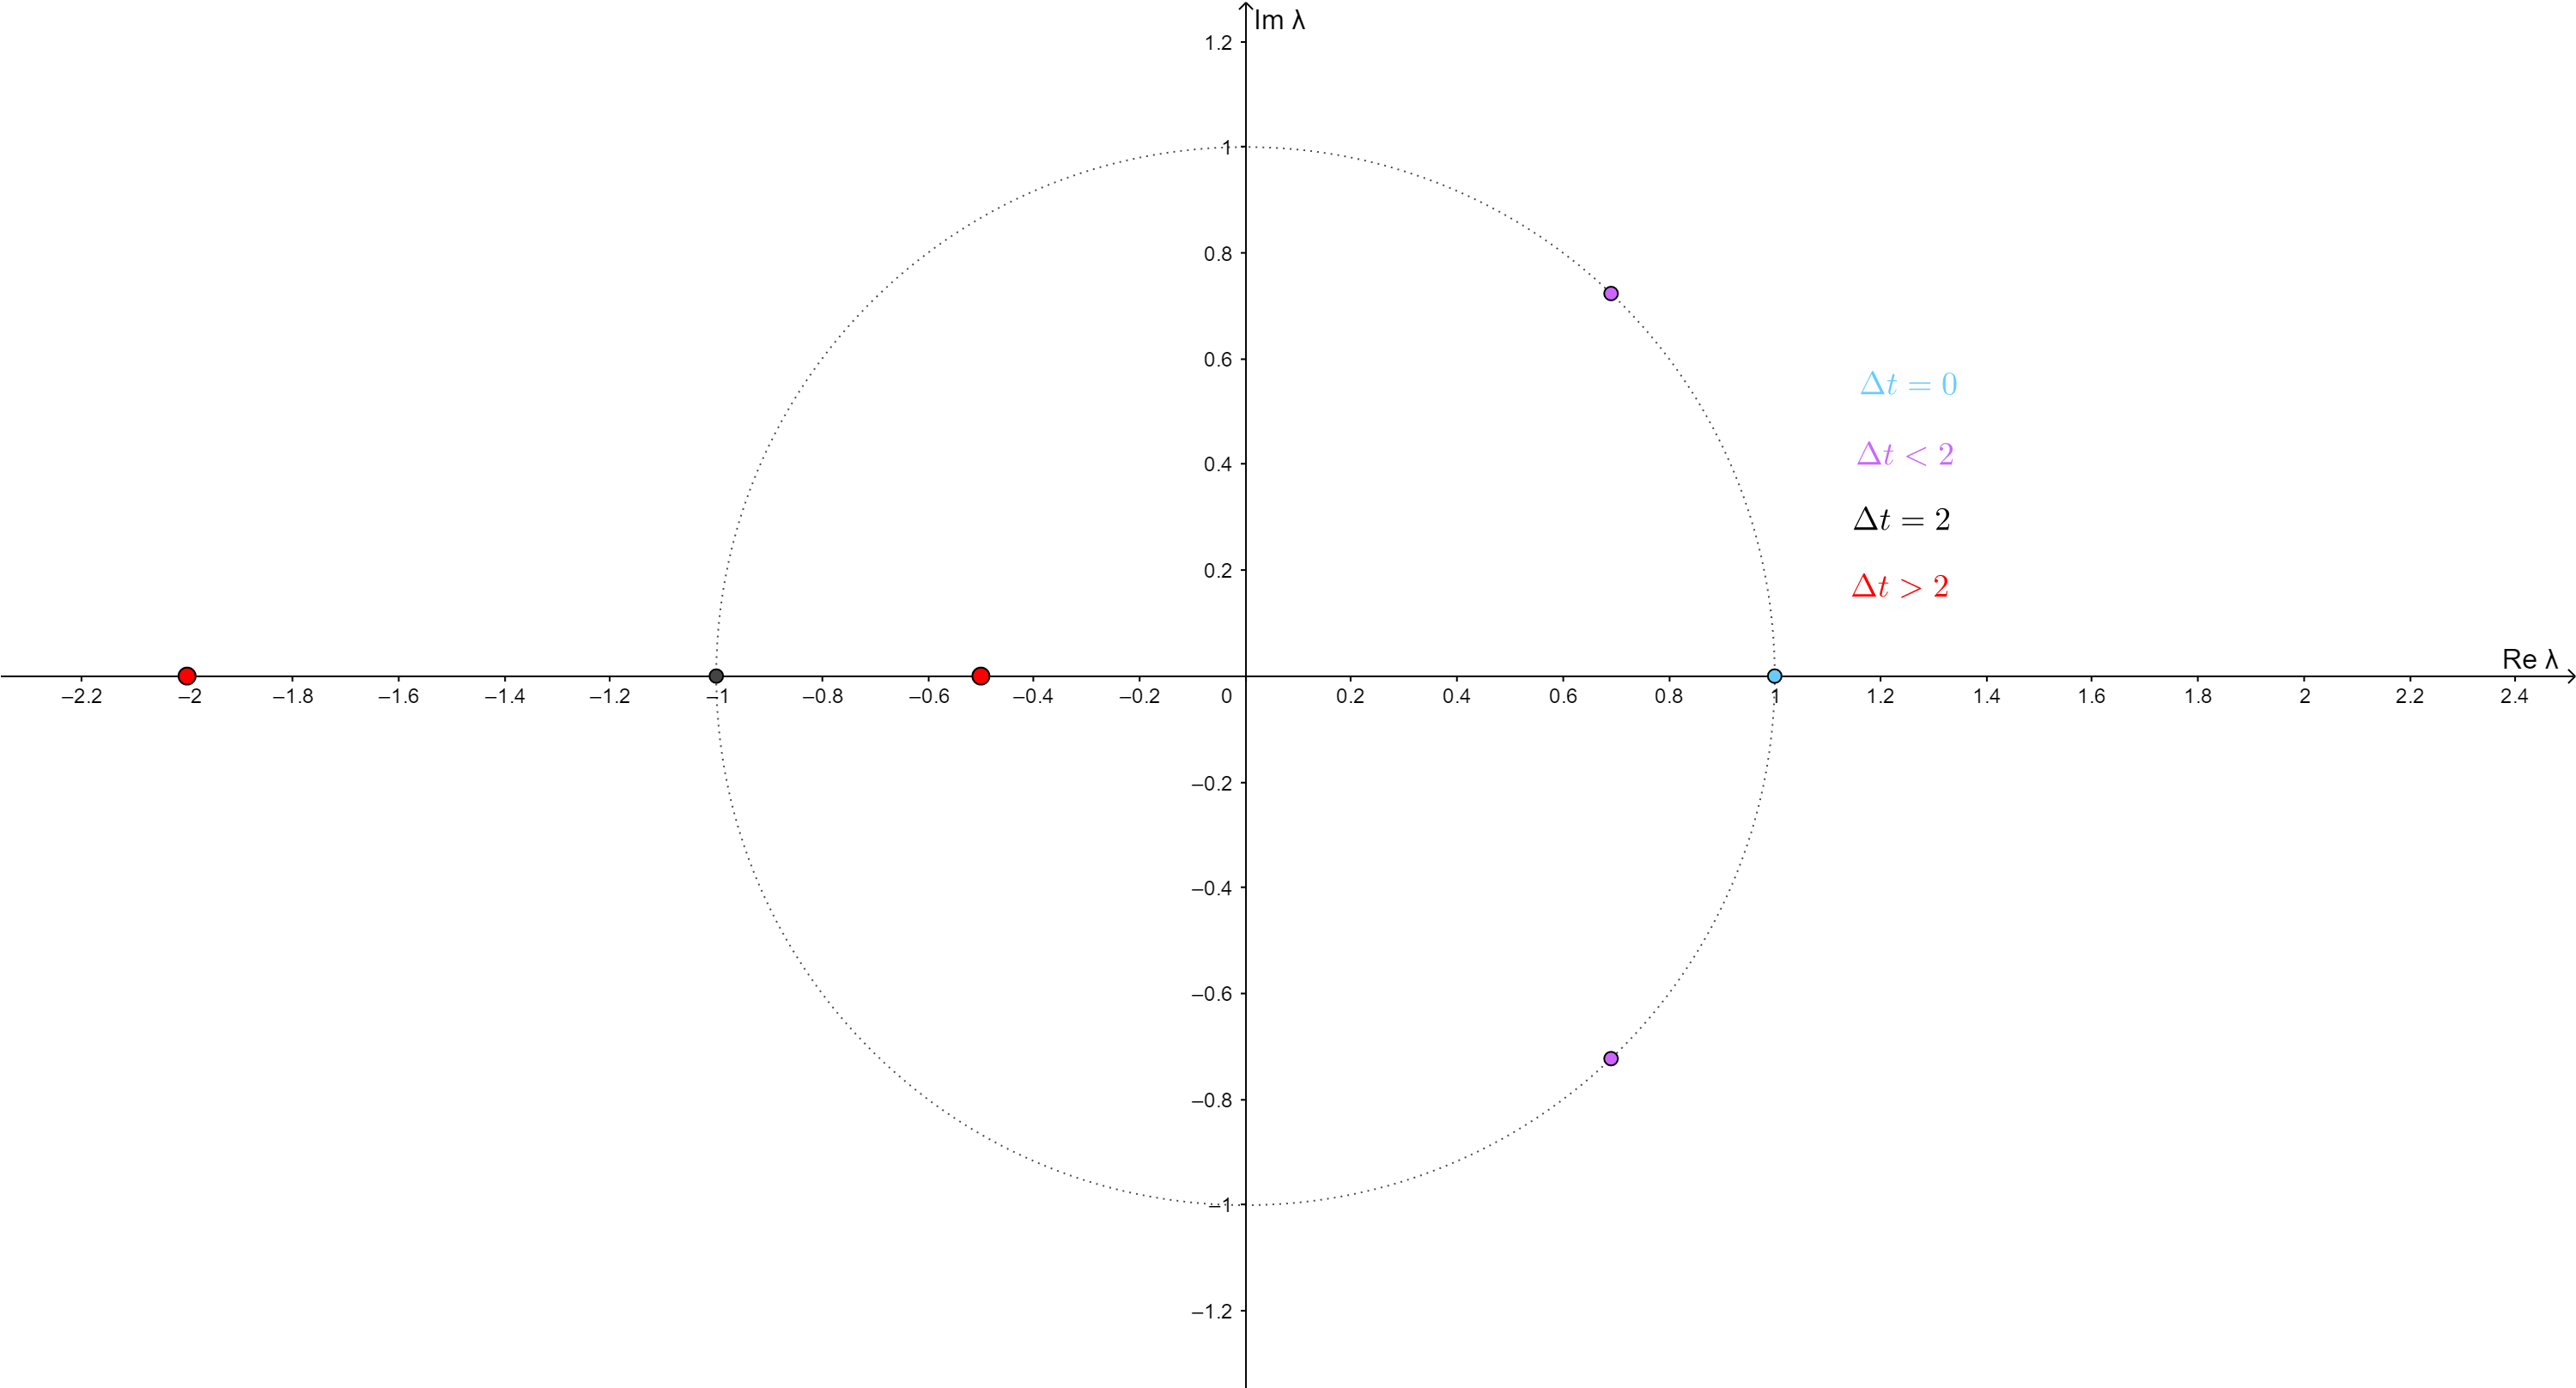
\includegraphics[scale=3.0]{Integrators/images/complexplane.png}
    \caption{Possible eigenvalues of the matrix $A$}
    \label{fig:complexplane}
\end{figure}
In the case where they are complex, their imaginary part is opposite and the real parts are equal.
After n steps:
\begin{equation}
    \begin{pmatrix}
      q' \\
      p'
    \end{pmatrix}
    = A^n
    \begin{pmatrix}
      q \\
      p
    \end{pmatrix}
\end{equation}
Check the behaviour for a large number of time steps ($n\xrightarrow{}\infty$):
\begin{itemize}
    \item if $A^n$ contains some infinite term, then the trajectory will diverge.
    \item if $A^n$ goes to 0, then the trajectory will converge (oscillate around the circular trajectory).
\end{itemize}
The eigenvalues of $A^n$ are equal to the eigenvalues of $A$ raised to the n-th power, therefore:
\begin{itemize}
    \item  $\lambda_1=\lambda_2=-1$: trajectory will oscillate\footnote{$\lambda_1=\lambda_2=1$ is the case when the timestep is equal to zero, therefore the system is not moving}. $$\Delta t = 2$$
    \item $\lambda_1> -1$, $\lambda_2< -1$ or $\lambda_2> -1$, $\lambda_1< -1$: matrix explodes, trajectory diverges. $$\Delta t > 2$$
    \item complex eigenvalues with unitary modulus: trajectory will oscillate.  $$\Delta t < 2$$
\end{itemize}
Threshold for stability of a numerical simulation:
\begin{equation}
    \Delta t < \frac{T}{\pi}
\end{equation}
This is the theoretical limit for the timestep, given the period. The criterion for the timestep is the same for Verlet and Velocity Verlet.
\subsection{Multiple springs}
Let us consider a situation where there are 3 particles with the same mass connected by springs with $k_1 >> k_2$. Let us estimate the maximum time step that should be used. The solution is to take the stiffest spring to impose the limit on the timestep, i.e., that gives the shortest timestep.
In general, this condition is given by the fastest degree of freedom, in other words, by the lightest possible atom with the stiffest spring. This is the way to find the upper bound for our timestep:
computing the period $2\pi \sqrt{\frac{m}{k}}$.
If energy is sufficiently conserved, this means that the timestep is small enough. It is difficult to predict a priori a good value of the timestep because there could be nonlinear potentials.


\chapter{Stochastic Differential Equations (SDE)}
    %Here there is the introduction

The general form of a first order differential equation is
\[
dx=A(x,t)dt,
\]
which can be expressed as 
\begin{equation}\label{s}
\Delta x=A(x,t)\Delta t
\end{equation}
in the limit $\Delta t \to 0$. In order to consider the noise, we can introduce in Eq. \eqref{s} a random component, that is
\begin{equation}\label{sd}
\Delta x=A(x,t)\Delta t+B(x,t)\sqrt{\Delta t}R(t),
\end{equation}

where $R(t)$ is a random variable drawn from a normal distribution with zero mean and unitary variance\footnote{We can always trace back to this case redefining $A(x,t)$ and $B(x,t)$ when it is drawn from a normal distribution with different mean and variance.}, while the term $B(x,t)$ represents the amplitude of the noise.

To understand why in the random component the power of $\Delta t$ is $1/2$, 
let us first consider just the deterministic part, that is the case in which $B(x,t)=0$ (and for simplicity $A(x,t)=A$, \emph{i.e.} $A(x,t)$ is constant). Thus, defining $\delta t = \Delta t/N$, we have
\[
\Delta x=A\sum_{i=1}^N\delta t=A\sum_{i=1}^N\frac{\Delta t}{N}=A\Delta t.
\]
This means that in this case the power of $\Delta t$ must be $1$, because it should be the same if we move once for $\Delta t$ or $N$ times for $\Delta t/N$.

In the case $A(x,t)=0$ and $B(x,t)=B$, \emph{i.e.} $B(x,t)$ is constant, we have
\[
\Delta x= B\sqrt{\Delta t}R.
\]
Defining again $\delta t = \Delta t/N$ and considering $N$ independent random variables $R_i$, each drawn from a normal distribution with zero mean and unitary variance, we obtain
\[
\Delta x= \sum_{i=1}^NB\sqrt{\delta t}R_i=B\sqrt{\delta t}\sum_{i=1}^NR_i=B\sqrt{\delta t}\sqrt{N}R=B\sqrt{\Delta t}R,
\]
since $\sum_{i=1}^NR_i$ is itself a normal random variable with mean $0$ and variance $N$.\footnote{In the limit $\Delta t \to 0$ the random variables $R_i$ could be drawn from whatever distribution with zero mean and unitary variance since for the Central Limit Theorem $\sum_{i=1}^NR_i$ will converge to a normal distribution with mean $0$ and variance $N$.} Consequently we obtain statistically the same result if we move once for $\Delta t$ or $N$ times for $\Delta t/N$, thus in this case the power of $\Delta t$ must be $1/2$.

Coming back to Eq. \eqref{sd}, in the limit $\Delta t \to 0$ the stochastic part dominates, nevertheless, the deterministic part cannot be neglected since the random contributions tend to cancel out among them.

In a more formal way, we can rephrase Eq. \eqref{sd} as follows.
\begin{equation}
dx=A(x,t)dt+B(x,t)dW(t),
\end{equation}
where $dW(t)$ is called Wiener noise. 
    \section{Ito chain rule}
\subsection{Formal derivation}
 We can write the discrete version of the SDE as:
 \begin{equation}
     \Delta x = A(x,t)\Delta t + B(x,t)\Delta W(t)
     \label{SDE}
 \end{equation}
 with the following conditions on $\Delta W$:
 \begin{equation}
     \begin{cases}
      \begin{aligned}
           & \langle \Delta W(t)\rangle = 0\\[2ex]
           & \langle \Delta W(t)\Delta W(t')\rangle = \delta_{t,t'}\Delta t
      \end{aligned}
     \end{cases}
 \end{equation}
 which enforce that the $\Delta W(t)$ are uncorrelated in time.\\
 We want now to find how to evolve this type of equation, that is we have $y(x)$ and we want to compute $\Delta y(x)$. We can expand $\Delta y(x)$ in series:
 \begin{equation}
 \begin{split}
     & y = y_0 + y'\Delta x + \frac{1}{2}y''\Delta x^2 + \frac{1}{6}y'''\Delta x^3 + \dots \\
     & \Delta y = y'\Delta x + \frac{1}{2}y''\Delta x^2 + \frac{1}{6}y'''\Delta x^3 + \dots 
 \end{split}
 \end{equation}
 and when $\Delta x$ is small we can keep only the terms up to the second order.\\
 We replace $\Delta x$ with Eq. \ref{SDE}, obtaining:
 \begin{equation}
     \Delta y = y'(A\Delta t + B\Delta W)+\frac{1}{2}y''(A^2\Delta t^2 + 2AB\Delta t\Delta W + B^2\Delta W^2) + \dots
 \end{equation}
 and we can check if some of the new terms are of an higher order than what we want to keep.\\
 Indeed we have that:
 \begin{equation}
     \begin{split}
         & A^2\Delta t^2 < A\Delta t\;\;for\;\;\Delta t\xrightarrow[]{} 0\\
         & 2AB\Delta t\Delta W < B\Delta W\;\;for\;\;\Delta t\xrightarrow[]{} 0
     \end{split}
 \end{equation}
 so we can neglect them.\\
 The remaining term ($B^2\Delta W^2 =B^2\Delta t R^2$) should be discarded on the basis that the power of $\Delta t$ is one and $R^2$ is a random number. Although we notice that we have $\langle R^2 \rangle = 1$, which means that the average contribution of this term is a drift, namely $B^2 \Delta t$. We can, then, keep just the term $B^2\Delta t$.\\
 Now we can write the equation that describes the evolution of $y(x)$, called \textbf{Ito chain rule}:
 \begin{equation}
 \Delta y = y'A(x,t)\Delta t + y'B(x,t)\Delta W + \frac{1}{2}y''B^2(x,t)\Delta t
     \label{Ito}
 \end{equation}
 we can see that the first two terms come from the classic chain rule, while the last is the one given by the stochastic nature of $x$.
 

 \subsection{Examples}
 
In this section we apply the Ito chain rule (Equation \ref{Ito}) to some practical examples: \\

\textbf{Example 1:} \begin{equation}
    dx = -xdt + dW \hspace{10mm} y = x^2
    \label{SDE_x_1}
\end{equation}

A numerical integration of the SDE on $x$ is the following:
\begin{figure}[H]
  \centering
  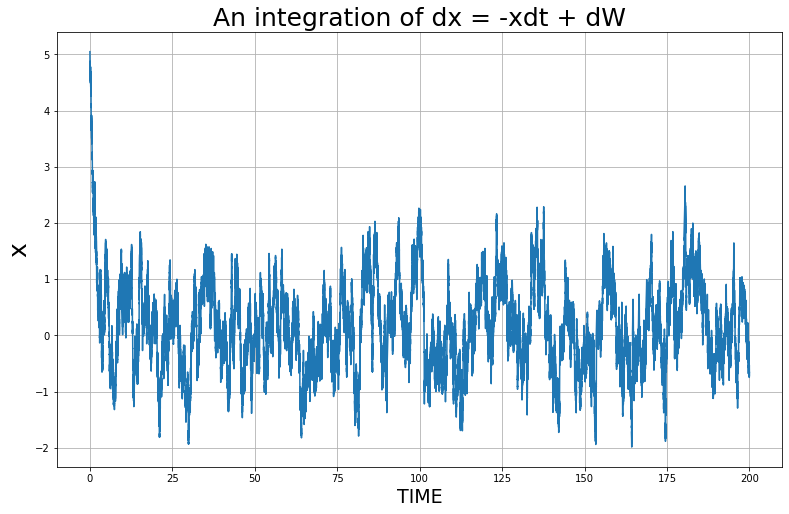
\includegraphics[width=0.8\textwidth]{SDE/Figures/SDEx.png}
  \caption{This numerical integration is produced using dt = 0.01, x(t=0) = 5, initializing the pseudo-random number generator with np.random.seed(1) and discarding the first element.} 
  \label{Fig:SDE_x_1}
\end{figure}

In this case we have:
 \begin{equation}
     \begin{split}
         & y' = 2x \\
         & y'' = 2 \\
         & A(x, t) = -x \\
         & B(x, t) = 1
     \end{split}
 \end{equation}

Applying Ito chain rule we get: 
  
\begin{align}
        \nonumber dy &= -2x^2dt + dt + 2xdW \\
        \nonumber &= (1-2x^2)dt + 2xdW\\
        \nonumber &= (1-2y)dt \pm 2\sqrt{y}dW\\
                  &= (1-2y)dt + 2\sqrt{y}dW
    \end{align}
\label{SDE_y_1}

Where in the last equation we used the fact that the plus and the minus sign generate the same SDE, since they are multiplied by an even random variable (i.e. gaussian random variable with zero mean).
We stress the fact that deriving a new SDE independent from $x$ (as in this case) is not always possible. \\
Equation (\ref{SDE_y_1}) might seem wrong because, if integrated with a finite time step $dt$, it can produce negative $y$'s, while we set $y = x^2$. This problem arises from the fact that we are using a finite time step. The smaller we set $dt$, the more it is unlikely to have negative $y$'s. So, instead of integrating Equation (\ref{SDE_y_1}), we simply square the values of Figure \ref{Fig:SDE_x_1} and produce the following figure: 
\begin{figure}[H]
  \centering
  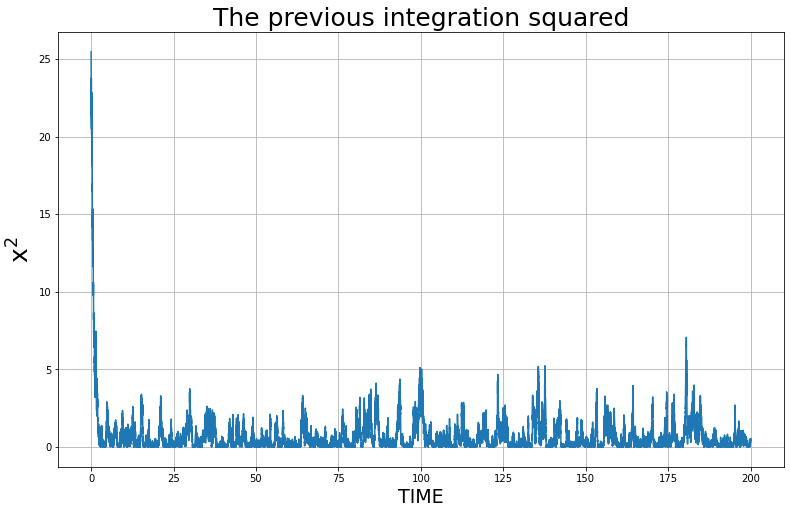
\includegraphics[width=0.8\textwidth]{SDE/Figures/SDEy.png}
  \caption{To produce this Figure we took the values in Figure \ref{Fig:SDE_x_1} and squared them.}
  \label{Fig:SDE_y}
\end{figure}

\textbf{Example 2:} 
\begin{equation}
    dx = BdW \hspace{10mm} y = e^x \hspace{10mm} B\hspace{1.5mm}constant
    \label{SDE_x_2}
\end{equation}
This is an example of Brownian motion/Random walk. 
3 numerical integrations of the same SDE on x are the following:
\begin{figure}[H]
  \centering
  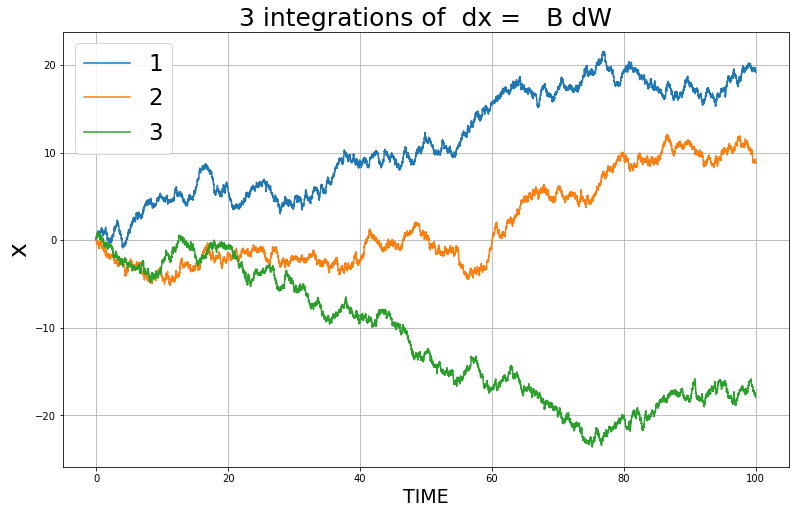
\includegraphics[width=0.8\textwidth]{SDE/Figures/SDEx_2.png}
  \caption{These numerical integrations are produced using dt = 0.01, x(t=0) = 0, initializing the pseudo-random number generator with np.random.seed(2) and discarding the first element.} 
  \label{Fig:SDE_x_2}
\end{figure}

In this case we have:
 \begin{equation}
     \begin{split}
         & y' = e^x = y \\
         & y'' = e^x = y \\
         & A(x, t) = 0 \\
         & B(x, t) = B
     \end{split}
 \end{equation}

Applying Ito chain rule we get: 
  
\begin{equation}
    dy = \frac{B^2y}{2}dt + BydW
    \label{SDE_y_2}
\end{equation}

It is worth noticing that, from Equation \ref{SDE_x_2}, we cannot expect $x$ to oscillate around a value as in the previous exercise (here there is only the random contribution). 

If we take the orange curve in Figure \ref{Fig:SDE_x_2} and apply the transformation y = $e^x$ we get:
\begin{figure}[H]
  \centering
  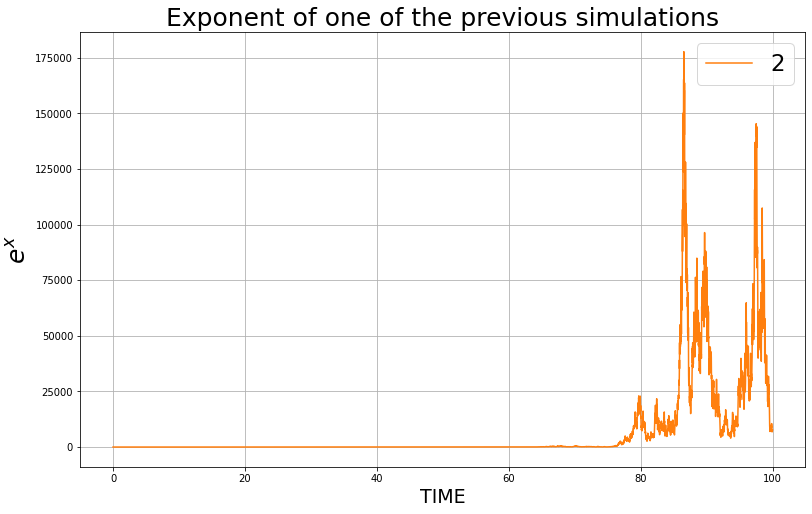
\includegraphics[width=0.8\textwidth]{SDE/Figures/SDEy_2.png}
  \caption{The exponent of each value of the orange simulation.}
  \label{Fig:SDE_x_2}
\end{figure}

\textbf{Example 3:} \begin{equation}
    dx_i = -x_i dt + dW_i \hspace{6mm} y = \sum_i x_i^2 \hspace{6mm} i = 1, ..., N
    \label{SDE_x_3}
\end{equation}

Defining $y_i$ = $x_i^2$ and  recalling Example 1 we write:
\begin{equation}
    dy_i = (1-2y_i)dt + 2\sqrt{y_i}dW_i
\end{equation}

Since $y$ is the sum of independent variables we can write:

\begin{align}
        \nonumber dy &= \sum_i dy_i = \sum_i (1-2y_i)dt + \sum_i 2\sqrt{y_i}dW_i \\
        \nonumber &= Ndt - 2\sum_i y_i dt + 2 \sum_i \sqrt{y_i}dW_i\\
        \nonumber &= Ndt - 2\sum_i y_i dt + 2 \sum_i \text{(Gaussian mean 0, variance $y_idt$)}\\
        \nonumber &= Ndt - 2y dt + 2\text{(Gaussian mean 0, variance $\sum_i y_idt$ = $ydt$)}\\
                  &= (N -2y) dt + 2\sqrt{y}dW
    \end{align}
\label{SDE_y_3}

We see that for N = 1 we recover the results of Exercise 1. \\

In this section we've always considered the random component to be normally distributed, but, in a stochastic process it could be possible to have different distributions that model the noise. In case of infinite variance we get discontinuity in the trajectory (the so-called Levy flights).


\subsection{Stratonovich formalism}
A stochastic differential equation can be represented also by using the so-called Stratonovich formalism, according to which
\begin{equation}\label{st}
\Delta x=A\Delta t+B(x+\frac{\Delta x}{2},t)\Delta W.
\end{equation}
As we can see from Eq. \eqref{st}, the random component $B$ is now evaluated in the middle point between the present position and the next position.

The same equation can therefore be expressed in two different ways depending on which formalism is used. In particular, we have
 \begin{align}
        \nonumber &dx=Adt+BdW \quad (\text{Ito})\\
        \nonumber &\dot{x}=A+B\eta \quad (\text{Stratonovich}),
    \end{align}
 where the coefficients $A,B$ are different for each formalism.
 
 


    \section{Fokker-Planck equation}
\subsection{Formula derivation}
Now we want to derive the Fokker-Planck equation, that corresponds to the Liouville equation when stochastic contributions are added to the system.\\
We start considering the Ito chain rule neglecting the time dependence of $A(x,t)$ and $B(x,t)$, that is 
\[
dy=y'A(x)dt+y'B(x)dW+\frac{1}{2}y''B^2(x)dt
\]
We now want to propagate the density on the phase space of different copies of the system, and in order to do so we need to count how many copies are present in a volume $\bar{x}$ of the phase space.

\begin{figure}[H]
  \centering
  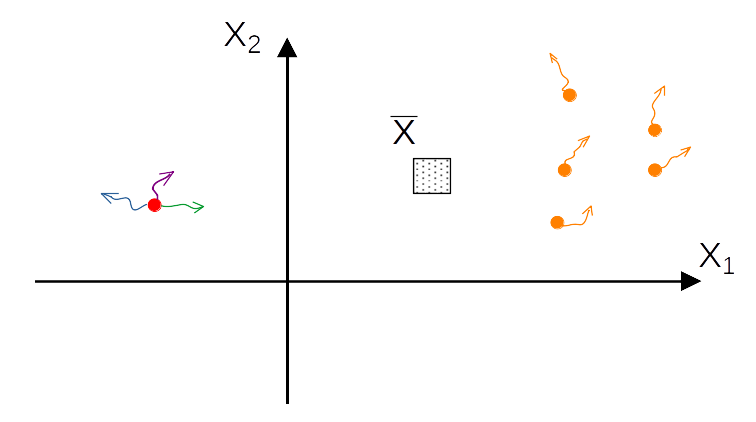
\includegraphics[width=0.8\textwidth]{SDE/Figures/Phase_space_Fokker.png}
  \caption{Two dimensional phase space.\\\hspace{\textwidth}
  Each point represent a specific configuration of the phase space. \\\hspace{\textwidth}
  As the {\color{red} red point} highlights, each point in the phase space can have different evolution due to randomness. On the other hand, we are usually interested in the evolution of an ensemble of many points ({\color{orange} orange points}). $\bar{x}$ represents a volume in the phase space.
  } 
  \label{Fig:Fokker_phase_space}
\end{figure}

Since we are dealing with continuous variables, in order to count the copies, we use the function $y(x)= \delta(x-\bar{x})$, then $y'(x)=\delta'(x-\bar{x}), y''(x)=\delta''(x-\bar{x})$.
Thus for a single trajectory we get
\begin{equation}
dy=\delta'(x-\bar{x})A(x)dt+\delta'(x-\bar{x})B(x)dW+\frac{1}{2}\delta''(x-\bar{x})B^2(x)dt.
\end{equation}
If we consider the double average we have:

\begin{equation}
    \begin{split}
        \langle dy \rangle &=\int dxP(x)\Big\langle\delta'(x-\bar{x})A(x)dt+\delta'(x-\bar{x})B(x)dW+\frac{1}{2}\delta''(x-\bar{x})B^2(x)dt\Big\rangle\\
        & =\int dxP(x)\left[\delta'(x-\bar{x})A(x)+\frac{1}{2}\delta''(x-\bar{x})B^2(x)\right]dt \label{eqn:sub}
    \end{split}
\end{equation}
where the integral represents the average over the phase space, ($P(x)$ is the probability of finding a copy in position $x$), while $\langle \rangle$ is the average among all the copies. The second term vanishes since the noises cancel out taking the average.
Assuming $x$ to be one dimensional and with no boundaries (\emph{i.e.} $x \in (-\infty,+\infty)$) we can compute the two terms in the integral of Eq. \eqref{eqn:sub}. For the first we have
\[
\int dx\left(P(x)A(x)\right)\delta'(x-\bar{x})\underbrace{=}_{\text{by parts}}-\int dx\left(\frac{\partial}{\partial x}P(x)A(x)\right)\delta(x-\bar{x})=-\frac{\partial}{\partial x}P(x)A(x)\bigg|_{x=\bar{x}}
\]
since $P(x)A(x)=0$ at $\pm\infty$. For the second term we have
\begin{equation*}
    \begin{split}
\frac{1}{2}\int dx\left(P(x)B^2(x)\right)\delta''(x-\bar{x})&\underbrace{=}_{\text{by parts}}-\frac{1}{2}\int dx\left(\frac{\partial}{\partial x}P(x)B^2(x)\right)\delta'(x-\bar{x})= \\
&\underbrace{=}_{\text{by parts}}+\frac{1}{2}\int dx \frac{\partial^2}{\partial x^2}\left(P(x)B^2(x)\right)\delta(x-\bar{x})= \\
&\,\,\,\,\,\,=\frac{1}{2}\frac{\partial^2}{\partial x^2}P(x)B^2(x)\bigg|_{x=\bar{x}}.
    \end{split}
\end{equation*}
Thus
\begin{equation}
\langle dy \rangle =\left[-\frac{\partial}{\partial x}\left(P(x,t)A(x)\right)+\frac{1}{2}\frac{\partial^2}{\partial x^2}\left( P(x,t)B^2(x)\right)\right]dt.
\end{equation}
Finally, since $\langle y \rangle =P(\bar{x})$, we get to the Fokker-Planck equation
\begin{equation}
\frac{\partial P}{\partial t}=-\frac{\partial}{\partial x}AP+\frac{1}{2}\frac{\partial^2}{\partial x^2}B^2P
\label{Fokker-Planck equation}
\end{equation}
which is expressed in a compact way neglecting the dependences on $t$ and $x$.




\subsection{Current density J}
If we define the current density $J$ as:
\[
J \equiv AP - \frac{1}{2} \frac{\partial}{\partial x}B^2 P
\]

We can re-write the Fokker-Planck equation (\ref{Fokker-Planck equation}) as a continuity equation:
\begin{equation}
\frac{\partial P}{\partial t} = - \frac{\partial J}{\partial x}.
\label{K-P continuity equation}
\end{equation}

In multiple dimensions:
\[
J_i \equiv A_iP - \frac{1}{2}\sum_j \frac{\partial}{\partial x_j} \left( \sum_k B_{ik}B_{jk} P \right)
\]

and the Fokker-Planck equation becomes:
\begin{equation}
\frac{\partial P}{\partial t} = - \sum_i \frac{\partial J_i}{\partial x_i} \hspace{5mm}\text{with }\hspace{3mm} dx_i = A_idt + \sum_j B_{ij} dW_j.
\label{K-P multidimentonal continuity equation}
\end{equation}


The introduction of $J$ allows us to connect the Fokker-Plank equation to Balance and Detailed Balance. \\
As we know Balance implies that the probability distribution $P$ doesn't change over time. So, using Fokker Plank we can say:
\[
\text{Balance} \hspace{2mm} \implies \hspace{2mm} \frac{\partial P}{\partial t} = 0 \hspace{2mm} \implies \hspace{2mm} \sum_i \frac{\partial J_i}{\partial x_i} = 0.
\]
So, there can be a flux of probability $\partial J_i$ along direction $i$, but the divergence of this flux must be zero. On the other hand, Detailed Balance enforces a stronger condition, that is, there is no flux along any component:
\[
\text{Detailed balance} \hspace{2mm} \implies \hspace{2mm} J_i = 0.
\]

Note that in 1D Detailed Balance and Balance imply the same condition. Indeed we can see that in an infinite domain, assuming Balance implies that $J=const$, but on the other hand $J\propto P$. Since $P(x\xrightarrow{}\pm \infty) = 0$, then $J = 0$. \\

\textbf{Example}:\\
\newline
We can apply the Fokker-Planck equation to a simple example:
\begin{equation*}
    dx = -xdt + dW
\end{equation*}
where we have $A=-x$ and $B=1$, so we obtain:
\begin{equation*}
\begin{split}
    & J=-xP-\frac{1}{2}\frac{\partial P}{\partial x}\\
    & \frac{\partial P}{\partial t} = \frac{\partial}{\partial x}(xP)+\frac{1}{2}\frac{\partial^2}{\partial x^2}P
    \end{split}
\end{equation*}
we can see in Fig. \ref{fok_ex} that the equation above \textit{flatten} $P(x)$, since around the peak the second derivative is negative, hence those points are decreased, while the points in the tails increase due to the positive second derivative. The ultimate result is a flat distribution.

\begin{figure}[H]
  \centering
  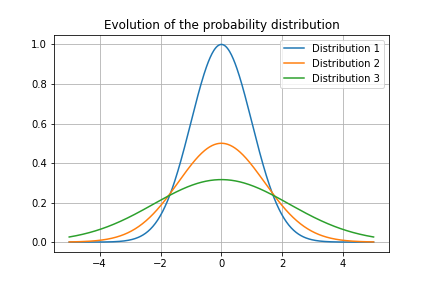
\includegraphics[width=0.7\textwidth]{SDE/Figures/fokker_example.png}
  \caption{Evolution of the distribution following Fokker-Planck. This distribution is just a graphical example, it should not be considered an accurate description of $P(x)$.}
  \label{fok_ex}
\end{figure}
 


\subsection{Example: Sampling from the Canonical Ensemble}
We can use the conditions for balance and detailed balance on $J$ in order to sample from the canonical ensemble.\\
We want to find the coefficient $A$ and $B$ for a given $P(x)$ such that:
\begin{equation*}
    AP - \frac{1}{2}\frac{\partial}{\partial x}\left( B^2 P \right) = 0
\end{equation*}
namely we want to enforce detailed balance.\\
If we fix $B=const$ we can find the correct value for $A$ solving:
\begin{equation*}
    A = \frac{1}{2}\frac{1}{P}\frac{\partial}{\partial x}\left( B^2 P \right)
\end{equation*}
which can be written as:
\begin{equation*}
    A = \frac{B^2}{2}\frac{1}{P}\frac{\partial P}{\partial x} = \frac{B^2}{2}\frac{\partial \log P}{\partial x}
\end{equation*}
where we used the fact that $B$ is constant.\\
We have that $P(x) \propto \exp(-\beta U(x))$, which gives:
\begin{equation*}
    A = -\frac{B^2}{2}\beta \frac{\partial U(x)}{\partial x}
\end{equation*}
Now we have everything we need to write the stochastic differential equation that rules the evolution of $x$. We call $B^2 = 2D$, where $D$ is the \textit{diffusion coefficient}, and we obtain:
\begin{equation}
    dx = -\frac{D}{k_B T}\frac{\partial}{\partial x}U(x)dt + \sqrt{2D}dW
\end{equation}
This equation is called \textit{Overdamped Langevin Equation} and we can see that for large $T$ the dynamic is dominated by the stochastic term.\\

In some particular situations we may also have:
\begin{equation*}
    dx = \sqrt{2D(x)}dW
\end{equation*}
with $A=0$ for simplicity. In this situation we obtain (as before $B^2 = 2D(x)$):
\begin{equation*}
    \frac{\partial D P}{\partial x} = 0
\end{equation*}
which entails that:
\begin{equation*}
    P(x) \propto \frac{1}{D(x)}
\end{equation*}
that can be interpreted as the fact that the particle spends more time in the regions where $D(x)$ is small.
\chapter{Thermostats}
    \section{Introduction}
In molecular dynamics, a thermostat is an algorithm built with the purpose of generating samples from a statistical ensemble at constant temperature $T$.
At this point, we know that the typical choice among the statistical ensembles, when simulating a real physical system, is the Canonical one, which allows fluctuations of the total energy under the constraint that its average remains constant over time.
Therefore, our aim will be to build thermostats which sample configurations drawn from the Canonical ensemble. 

Before entering in the implementation of these algorithms, let's recall some of the main features of the ensemble we are interested in.

\subsection{Recap of the Canonical ensemble}
The probability distribution related to the Canonical ensemble, as defined in Chapter 1 (1.36), is given by
\begin{equation}
     P(x)=\frac{e^{-\beta H(x)}}{Z}
\end{equation}
with 
\begin{equation}
     Z=\int_ {}^{} e^{-\beta H(x)}dx
\label{zetafunc}
\end{equation} 

\par Is important to remember that here $x$ represents a vector that contains the position and momenta of all the particles of the system, so the integral (5.2) is taken over all the points composing the phase space of our system. 

As we have already seen, this formulation allows us to compute the average of a generic observable $A(x)$ as
\begin{equation}
     \langle A \rangle =\int_ {}^{} P(x)A(x)dx,
\end{equation}

and, as a consequence, its variation with respect to the temperature as
\begin{equation}
    \frac{\partial \langle A \rangle}{\partial T}=-\frac{1}{k_B T^2} (-\langle HA \rangle+\langle H \rangle\langle A\rangle). 
\end{equation}

Some relevant examples are the derivatives of the average values of:
\begin{itemize}
    \item The total energy $H$
    \begin{equation}
      \frac{\partial \langle H \rangle}{\partial T}=\frac{1}{k_B T^2} (\langle H^2\rangle-\langle H\rangle^2)=\frac{1}{k_B T^2}\sigma_H^2
    \end{equation} 
    which is proportional to the variance of $H$ (i.e. the amplitude of its fluctuations) and which can be physically interpreted as the amount of energy needed in order for the temperature to increase by 1 degree, i.e. the Heat capacity; 
    \item The potential energy $U$
    \begin{equation}
        \frac{\partial \langle U \rangle}{\partial T}=\frac{1}{k_B T^2} (\langle U^2 \rangle -\langle U \rangle^2)=\frac{1}{k_B T^2}\sigma_U^2 ;
    \end{equation}
    \item the kinetic energy $K$
    \begin{equation}
        \frac{\partial \langle K \rangle}{\partial T}=\frac{1}{k_B T^2} (\langle K^2\rangle-\langle K \rangle^2)=\frac{1}{k_B T^2}\sigma_K^2 .
    \end{equation}
\end{itemize}

In particular, the last two results are obtained exploiting the feature of the Hamiltonian of the majority of the systems we are interested in, built as the sum of a kinetic contribution \begin{math} K(p)=\sum_{i=1}^{N_a} \frac{{p_i}^2}{2m_i} \end{math}, which depends only on the momenta $p_i$ of the particles, and a potential contribution $U(q)$, specific of the system, which depends only on the positions $q_i$. 

This composition of the Hamiltonian makes the probability distribution $P(x=p,q)$ factorizable into two separate parts: \begin{math}P_K(p) \propto e^{-\beta \sum_{i=1}^{N_a} \frac{p_i^2}{2m_i}} \end{math} (which is a gaussian) and $P_U(q)$.

Then, from  $P_K(p)$ we can obtain the probability distribution of the kinetic energies $P_K(K)$, which is not a gaussian (because as $K<0$, $P_K$ is identically equal to $0$), but a Gamma distribution
\begin{equation}
    P_K(K) \propto K^{N_F/2 -1}e^{-\beta K}
\end{equation}
where $N_F=3N_a$ is the number of degrees of freedom, with average
\begin{equation}
    <K>=\frac{3}{2} N_a k_B T \implies \frac{\partial <K>}{\partial T}=\frac{3}{2} N_a k_B
\end{equation}

and width (from (5.7) and (5.8))
\begin{equation}
    \sigma_K=\sqrt{k_B T^2 \frac{\partial <K>}{\partial T}}=\sqrt{\frac{3}{2} N_a k_B^2 T^2}= \sqrt{<K>^2 \frac{2}{3 N_a}}.
\end{equation}
In particular, the factor $K^{N_F/2 -1}$ is in some way related to the density of state: this explains why negative kinetic energies are not allowed ($P_K(K<0)=0$) and why, without the compensation of the Boltzmann factor \begin{math} e^{-\beta K} \end{math}, high kinetic energies would be more likely.
A qualitative description of the behaviour of $P_K(K)$ can be seen in Figure \ref{fig:kinetic distribution}

\begin{figure}
    \centering
    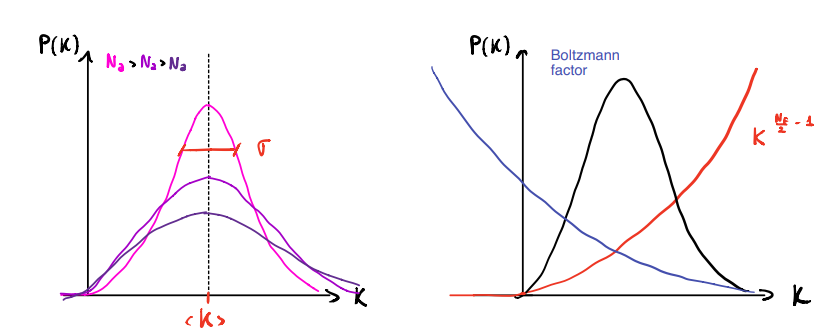
\includegraphics[width=0.7\textwidth]{Thermostats/images/kinetic distribution.PNG}
    \caption{On the left: qualitative behaviour of the Gamma distribution $P_K(K)$ at different values of $N_a$, always centered in the same value in order to compare visually the different shapes. On the right: qualitative behaviour of the two factors that compose $P_K(K)$, whose coexistence leads to the typical shape of the Gamma distribution.}
    \label{fig:kinetic distribution}
\end{figure}

\section{Algorithms}

As mentioned in the Introduction, the two main properties of the thermostats we want to implement are:
\begin{itemize}
    \item Equilibration of the system to a target value of the temperature $\bar T$, that, after an early transient, have to remain constant;
    \item Production of configurations drawn from the Canonical ensemble.
\end{itemize}

First of all, we have seen, as one of the main results of the theoretical description of the Canonical ensemble, that \begin{math} <K> \propto T \end{math}. 
Therefore, we can think about controlling the value of the temperature through the control of the kinetic energy $K(p)$, which will have to reach the target value $\bar K \propto \bar T$. This control on $K(p)$ can be realized imposing proper variations of $K(p)$ itself, in such a way that $<K>= \bar K$. 

But this will not be sufficient in order to satisfy the second request: in fact, in order for our simulation to produce canonical configurations, we need also the fluctuations on $K(p)$ to be coherent with the canonical distribution, and so equal to its variance $\sigma_K^2$.

As a consequence of these requirements, the main idea to implement thermostats is by choosing a rule for the variation of $K(p)$, and evolving the system through a modified version of Hamilton equations, which will determine variations of potential energy $U(q)$ in such a way that the ones of $K(p)$ are balanced, and so that the total energy is approximately conserved.


\subsection{Trial and error}

The first attempt, which can not be called an actual algorithm, but is useful to introduce us to the logic underlying thermostats, is the "Trial and error". 
It exploits the behaviour of the simulation to set the proper value of the initialization $K_0$ which, after a transient, will lead to the target value \begin{math} \bar K \end{math} (and so to the target value \begin{math} \bar T \end{math}).

At first, in fact, we could try initializating the kinetic energy at its target value. Unfortunately, starting the simulation we would see that $K$ doesn't remain constant at $\bar K$, but equilibrates to a different value.

So, we could think of starting a new simulation from a different $K_0$, shifted from the previous by the difference between $\bar K$ and the previous equilibration value.
Typically, the optimal result can not be reached in a unique attempt, but after various iterations, which can be stopped when the difference between $\bar K$ and the new equilibration value of $K$ is small enough.

\begin{figure}
    \centering
    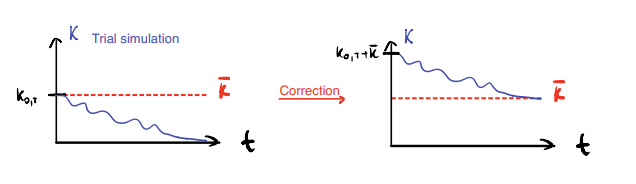
\includegraphics[width=0.7\textwidth]{Thermostats/images/Trial and error.PNG}
    \caption{The first image represent the Trial simulation, where the kinetic energy is initialized to its target value. The second represent the correct simulation, where the initialization is set to that value from which, after the equilibration, the kinetic energy reaches the target value.}
    \label{fig:trial and error}
\end{figure}

In Figure \ref{fig:trial and error} we see how this procedure would look if a unique attempt would be sufficient.

Unfortunately, as we can imagine looking at the triviality of this algorithm, this is not a suitable choice for implementing a thermostat.

\subsection{Velocity rescaling}
The Velocity rescaling algorithm is based on the following idea:
\begin{itemize}
    \item Given an initial configuration of the system, we run a number \textit {stride} of steps using a Hamilton equations integrator, like, for example, Velocity Verlet;
    \item We check the istantaneous value of $K$ and we change it rescaling it by a factor that makes it equal to the target value $\bar K=\frac{3}{2}N_a K_B \bar T$.
\end{itemize}

A pseudocode representing these operations would be:
\begin{algorithm}[H]\label{velocity_rescaling}
			\caption{Velocity rescaling algorithm}
			\begin{algorithmic}[1]
				\For{$i step\; inrange (nsteps)$}
    				\State $p+=f*\Delta t/2$
    				\State $q+=p*\Delta t/m$
    				\State $p+=f*\Delta t/2$
    				\If{$i step\%stride==0$}
    				    \State $K= \frac{\sum_{i}{p_i^2}}{{2m_i}}$
    				    \State $p* = \sqrt{\frac{\Bar{K}}{K}}$
    				\EndIf
				\EndFor
			\end{algorithmic}
		\end{algorithm}

\begin{figure}
    \centering
    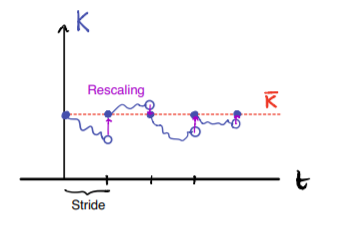
\includegraphics[width=0.7\textwidth]{Thermostats/images/velocity rescaling.PNG}
    \caption{Example of a trajectory $K(t)$ produced using the Velocity rescaling thermostat.}
    \label{fig:velocity rescaling}
\end{figure}		

As we can see, in this case the change in the kinetic energy is made on its total value, and not on the specific values $K_i$ of the single particles: this feature defines the so called \textit {Global thermostats}.

Although, as also qualitatively represented in Figure \ref{fig:velocity rescaling}, this algorithm works well in the equilibration to the target value $\bar K$, reached in a time interval $\propto {\textit {stride}}$, this is not an optimal choice for two main reasons: first of all, the distribution we are sampling from is unknown, and certainly it is not the canonical since the fluctuations of $K$ are not the proper ones (see Figure \ref{fig:fluctuations}); then, the trajectory is discontinuous, and this does not allow us to convert the algorithm into a differential equation.

\begin{figure}
    \centering
    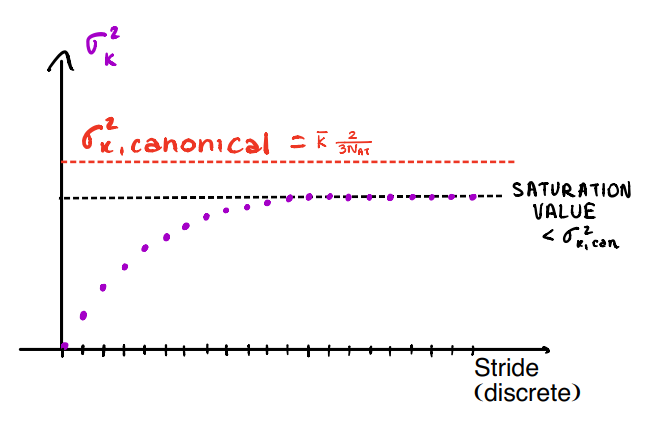
\includegraphics[width=0.7\textwidth]{Thermostats/images/fluctuations.PNG}
    \caption{Behaviour of $\sigma_K^2$ as a function of \textit {stride}. If \textit {stride} is small, the trajectory is smoother and $<K>=\bar K$, but the fluctuations are too small. If \textit{stride} is too big, the fluctuations will reach a saturation value smaller than the correct one, and also $K$ doesn't reach the target: in fact, this choice would basically correspond to evolving the system according to Velocity Verlet, which guarantees the conservation of the total energy and then produces configurations drawn from the Microcanonical distribution. }
    \label{fig:fluctuations}
\end{figure}

\subsection{Berendsen thermostat}
The problem of discontinuity in Velocity rescaling algorithm is soon solved by the Berendsen thermostat, which can be interpreted as its "continuous version".

It is based on the idea of modifying $K$ at each step, rescaling it by a properly weighted sum of the current value and the target value.

In practice, this operation would consist into the multiplication of the current value of the momentum $p$ by a factor
\begin{equation}
    F={\sqrt{\frac{c_1K+c_2 \bar K}{K}}}.
\end{equation}

In particular, the choice of the weights ${c_1}$ and ${c_2}$ has to guarantee the following properties:
\begin{itemize}
    \item $c_1+c_2=1$
    since, when $K=\bar K$, the factor F must be equal to 1, because the target value has been reached, and then we do not have to modify the current value;
    \item the limit $c_1 \rightarrow 1$ ( $\implies c_2 \rightarrow 0$), which represents the absence of the thermostat (since there are no corrections to the current values $p$) should coincide with the limit case of $\textit{stride}=\tau \rightarrow \infty$ in Velocity rescaling;
    \item the limit $c_2 \rightarrow 1$ ($\implies c_1 \rightarrow 0$), which basically respresents the application of Velocity rescaling at each step, should coincide with the limit case of $\textit{stride}=\tau \rightarrow 0$.
\end{itemize}

A choice which guarantees the latter requests is:
\begin{equation}
   c_1=e^{-{\frac{\Delta t}{\tau}}} ;\quad
      c_2=1-c_1=1-e^{-{\frac{\Delta t}{\tau}}}
\end{equation}

At this point, we can try converting the algorithm into a differential equation:
\begin{multline*}
    K_{new}={\frac{e^{-{\frac{\Delta t}{\tau}}}K+\left(1-e^{-{\frac{\Delta t}{\tau}}}\right) \bar K}{K}}K \\ 
    \implies \Delta K=K_{new}-K=e^{-{\frac{\Delta t}{\tau}}}K + (1-e^{-{\frac{\Delta t}{\tau}}}) \bar K - K \\
    = (1-e^{-{\frac{\Delta t}{\tau}}} )(\bar K -K) 
\end{multline*}

Then, performing the infinitesimal limit:
\begin{equation*}
    \lim_{{\Delta t}\to 0} \Delta K = (1-1+\frac{\Delta t}{\tau} + \textit{h.o.t})(\bar K-K)=\frac{\Delta t}{\tau}(\bar K-K)
\end{equation*}

\begin{equation}
    \implies dK=dt \frac{(\bar K-K)}{\tau}
\end{equation}

that is actually a differential equation. This means its solution, i.e. $K(t)$, is continuous, and then we can say that the issue we had with Velocity rescaling is solved.

Another advantage with respect to Velocity rescaling is that now we have a control parameter $\tau$, which, differently from \textit{stride}, has a physical interpretation:
it is the relaxation time of the system, and gives a qualitative measure of the thermal inertia of it, since the greater is $\tau$, the more difficult will be to change $K$, namely $T$.

Moreover, as a smoother version of Velocity rescaling, Berendsen's is itself a global thermostat.

So, in conclusion, one of the main advantages of using this algorithm is that the trajectories it produces are continuous, but it is not the only one. In fact, according to the huge number of citations of the original paper by Berendsen (1984), it is probably the most used thermostat, and this is due to a series of properties: it empirically equilibrates well; it is easy to understand; it is efficient. Regarding the efficiency, this is what actually makes people prefer this algorithm to more exact ones like, for example, Hybrid Montecarlo: indeed, the approximation makes Berendsen thermostat quicker in simulating very large systems, for  which a more accurate algorithm would take a too long time.

However, this algorithm does not sample configurations from the canonical distribution. In fact, even if balance is satisfied, because a stationary distribution can be reached, this is not the canonical one, and this is due to the fact that $K$ does not respect the proper fluctuations. Detailed balance is instead not guaranteed, because $K$ is forced to reach $\bar K$ and a time-reversed trajectory is not even possible.




    \section{Maximum entropy principle and microcanonical ensemble}
As before, consider a system divided in two compartments with energies $E_1$ and $E_2$. The two subsystems can exchange energy, but the sum $E_1+E_2 = E$ is fixed. We have already demonstrated that the phase space of the system at the equilibrium is given by 
\begin{equation}
    \Gamma_{1+2}(E) = \Gamma_1(E_1^*)\,\Gamma_2(E-E_1^*),
\end{equation}
where $E_1^*$ is the energy that maximizes $\Gamma_{1+2}$. This relation is clearer if one thinks of $\Gamma_i$ as the degeneracy of a state with an energy $E_i$. The equilibrium condition then becomes
\begin{equation}
    \frac{\partial \Gamma_{1+2}}{\partial E_1}\bigg|_{E_1^*} = \frac{\partial \Gamma_1(E_1)}{\partial E_1} \Gamma_2(E - E_1) + \Gamma_1(E_1)\frac{\partial \Gamma_2(E - E_1)}{\partial E_1} = 0.
\end{equation}
Since we have the constraint $E_2 = E-E_1$, we can take the derivative of $\Gamma_2$ with respect to $E_2$, changing its sign. Ordering the terms and multiplying by the Boltzmann constant $k_B$ we obtain
\begin{equation}
    \frac{k_B}{\Gamma_1} \frac{\partial \Gamma_1}{\partial E_1} = \frac{k_B}{\Gamma_2} \frac{\partial \Gamma_2}{\partial E_2} \: \Longrightarrow \:
    k_B \frac{\partial (\ln{\Gamma_1})}{\partial E_1} = k_B \frac{\partial (\ln{\Gamma_2})}{\partial E_2}
\end{equation}
and $k_B\ln{\Gamma}$ was our definition of entropy $S$. So the equilibrium condition is 
\begin{equation}
    \frac{\partial S_1}{\partial E_1} = \frac{\partial S_2}{\partial E_2}
\end{equation}
which is equivalent to having the same temperature. \\ \\

Entropy is an observable, so its expected value can be written as $S = \int d\Gamma \rho f(q,p)$ for a certain function $f$ of positions and momenta. From an analogy with probability theory and Shannon entropy, entropy turns out to be
\begin{equation}
    S = -\int d\Gamma \rho \ln{\rho}.
\end{equation}
which is also equal to $S=\ln{\Gamma}$ (for $k_B=1$).
We don't give a formal proof of this statement, but we show that it gives correct results in two particular limit cases:
\begin{itemize}
    \item case 1: $n$ energy levels, with $p_1 = 1$ and $p_{i\neq 1} = 0 \: \Rightarrow \: S=0$. \\
    \item case 2: $p_i = 1/n$ for all $i \: \Rightarrow \: S= -\frac{1}{n}\ln(\frac{1}{n})^n = \ln{n}$.
\end{itemize}
The maximum entropy principle states that a system in equilibrium tends to maximize entropy, given the constraints, for every probability density $\rho$. For the microcanonical ensemble, we consider the following constraints for $\rho$:
\begin{gather}
    \int d\Gamma \rho = 1 \: \Rightarrow \: \text{normalization} \\
    \rho(\mathbf{q},\mathbf{p}) = 0 \: \text{if} \: H(\mathbf{q},\mathbf{p}) \not\in (E,E+\Delta).
\end{gather}
For $k_B=1$, $S = -\int d\Gamma \rho \ln{\rho}$ and introducing the Lagrange multiplier $\lambda$ we can construct the functional
\begin{equation}
    \mathcal{F}[\rho] = -\int d\Gamma (\rho \ln{\rho} - \lambda\rho)
\end{equation}
and our goal is to find $\rho^*$ that makes it stationary. More explicitly, we want the functional differential
\begin{equation}
    \partial\mathcal{F}[\rho^*] \equiv \mathcal{F}[\rho^*+\delta\rho] - \mathcal{F}[\rho^*]
\end{equation}
with no linear terms in $\delta\rho$. Then we get
\begin{align}
\label{eq:rho_micro}
    \partial\mathcal{F}[\rho^*] &= -\int d\Gamma [(\rho^*+\delta\rho)\ln(\rho^*+\delta\rho) - \lambda(\rho^*+\delta\rho)] + \int d\Gamma (\rho^*\ln\rho^* - \lambda\rho^*) \nonumber \\
    &= -\int d\Gamma (\delta\rho\ln{\rho^*}+\delta\rho-\lambda\,\delta\rho) + h.o.t. \nonumber \\
    &= -\int d\Gamma \delta\rho \,(\ln{\rho^*}+1-\lambda) = 0
\end{align}
where in the second line we have used the fact that 
\begin{equation}
    \ln(\rho^*+\delta\rho) \simeq \ln{\rho^*} + \frac{\delta\rho}{\rho^*} + h.o.t.
\end{equation}
Since eq. (\ref{eq:rho_micro}) has to hold for every $\delta\rho$, the integrand must be null, i.e.
\begin{equation}
    \ln{\rho^*}(\mathbf{q},\mathbf{p}) = \lambda-1
\end{equation}
that does not depend on $\mathbf{q}$ and $\mathbf{p}$, so we obtain a uniform \textit{a priori} probability. This is due to the fact that we had no constraints, except for the normalization of the probability density. We can repeat the same calculation adding the constraint 
\begin{equation}
    \int d\Gamma \rho\,H = \bar{E}
\end{equation}
that corresponds to the canonical ensemble.




    %by Elena C. WORK IN PROGRESS
\subsection{Leapfrog Algorithm}
The Velocity Verlet algorithm shown previously (Algorithm \ref{alg:velocity_verlet}) can be modified to reduce the computational cost.\\ In particular, compute a force is quite expensive: computing the force twice will require twice the simulation time. One solution to reduce the computational cost is to merge the momenta shifts together (using the same value of the force): this leads to a slightly faster simulation, but on the other side this kills the possibility of printing the values of p and q at the same time (access to the phase space). This solution is called \textbf{Leapfrog algorithm}.\\
\begin{algorithm}[H]
			\caption{Leapfrog algorithm}
			\label{alg:leapfrog}
			\begin{algorithmic}[1]
			    \State $p=p+f*\Delta t/2$	\For{$i=1,...,nsteps$}
    			\State	$q=q+p/m \Delta t$
                 \State	$f=force(q)$
    			\State	$p=p+f*\Delta t$
				\EndFor
			\end{algorithmic}
		\end{algorithm}
Momentum and position are moved in an alternate way: at the end of a cycle, we do not find the values of the positions and momenta at the same timestep, they are found at a difference of half timestep. Slightly faster than Velocity Verlet, not very significant. 
\begin{figure}[H]
    \centering
    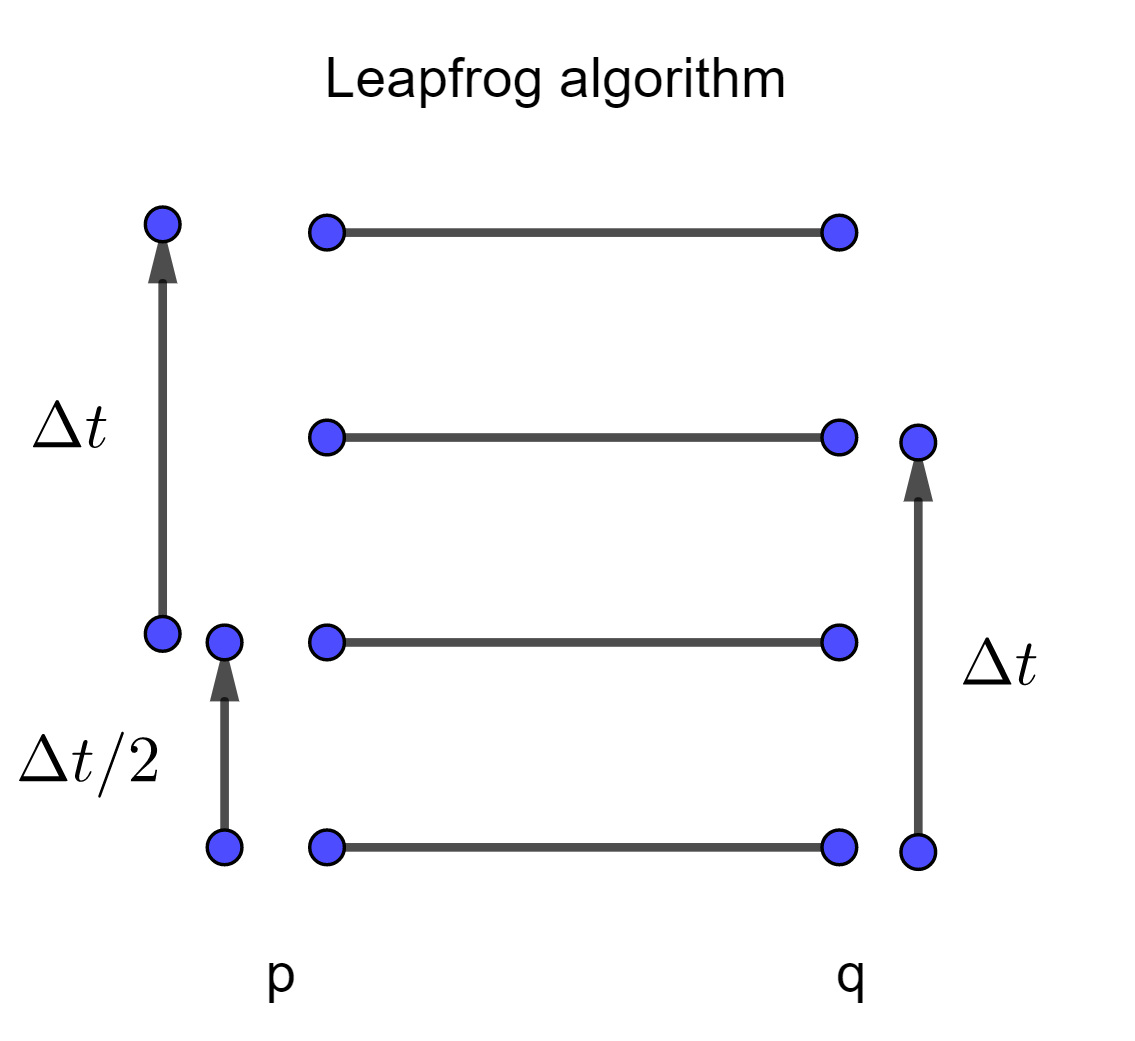
\includegraphics[width=50mm,scale=0.5]{Integrators/images/leapfrog.png}
    \caption{Scheme of the leapfrog algorithm}
    \label{fig:leapfrog}
\end{figure}
\subsection{Position Verlet}
Another alternative to the Velocity Verlet algorithm it is the so-called \textbf{Position Verlet algorithm}.
\begin{algorithm}[H]
			\caption{Position Verlet}
			\label{alg:position_verlet}
			\begin{algorithmic}[1]
        	\For{$i=1,...,nsteps$}
			\State	$q=q+p/m* \Delta t/2$
			\State	$f=force(q)$
			\State	$p=p+f*\Delta t$
			\State	$q=q+p/m* \Delta t/2$
				\EndFor
			\end{algorithmic}
		\end{algorithm}
This algorithm is the swapped version of Velocity Verlet, where the free particle is evolved for half timestep, then the infinite mass system is evolved for one timestep, then the free particle again for half timestep. 
\begin{itemize}
    \item \textbf{Advantages:} the force is computed only once, which is computationally advantageous (only one update of the momentum).
    \item \textbf{Disadvantages:} I cannot print the total energy. Potential energy needs to be computed with a similar procedure to the computation of forces (very expensive). Therefore, it is more convenient to compute forces and energies at the same time, but it is not possible with Position Verlet. Moreover, this algorithm is less used than Velocity Verlet, which is the simplest one.
\end{itemize}

\subsection{Other considerations on the Velocity Verlet algorithm}
Let us recall the Velocity Verlet algorithm:
    \begin{equation}\label{velocityverlet}
            \begin{cases}
                q(t+\Delta t)= q(t)+\frac{p(t)}{m}\Delta t+ \frac{f(t)}{m}\frac{\Delta t^2}{2}\\
                p(t+\Delta t)= p(t)+\frac{f(t)}{2}\Delta t+ \frac{f(t+\Delta t)}{2}\Delta t
            \end{cases}
            \end{equation}
Let's prove that the trajectories obtained with Velocity Verlet are equivalent to those obtained with Verlet algorithm. Trajectories are exactly time reversible, which means that we are allowed to compute $q(t-\Delta t)$ changing the sign of $\Delta t$ in the first equation \ref{velocityverlet}:
\begin{equation}\label{t-dt}
q(t-\Delta t)= q(t)-\frac{p(t)}{m}\Delta t+ \frac{f(t)}{m}\frac{\Delta t^2}{2}
\end{equation}
Let us sum $q(t-\Delta t)$ and $q(t+\Delta t)$ (first eq. \ref{velocityverlet} and eq. \ref{t-dt}):
\begin{equation*}
    q(t-\Delta t)+q(t+\Delta t)=2q(t)+\frac{f(t)}{m}\Delta t^2
\end{equation*}
This is consistent because equation \ref{velocityverlet} for the positions resembles a Taylor expansion of q.  The introduction of operator formalism is significant only for the sake of studying the evolution of momenta, while the evolution of positions is equivalent to the one obtained with the Verlet algorithm. 
In fact, the same trajectory results from the application of Verlet and Velocity Verlet algorithms.\\
Differences between the two algorithms are found by the fact that the Verlet algorithm considers differences between positions (current position $q(t_0)$ minus previous position $q(t_0-\Delta t$)): this leads to large round-off errors. Meanwhile, this problem is not present in Velocity Verlet, which is more numerically stable. Moreover, Velocity Verlet already includes a definition of the velocity, not present in Verlet algorithm: in the former case it is possible to compute the total energy and check if it is conserved.
We recall the properties of Velocity Verlet already discussed in section \ref{chapt:properites_vel_verlet}:
\begin{itemize}
\item \textbf{Trajectory is time reversible.}
\item \textbf{Volume in phase space is conserved.}
\item \textbf{Energy is not conserved}
\end{itemize}
Let us check the latter property for a simple example.
\subsubsection{Harmonic oscillator}
Force is given by 
\begin{equation*}
    f=- k q
\end{equation*}
Change slightly the notation:
\begin{equation*}
    \begin{cases}
        q=q(t)\\
        q'=q(t+\Delta t)
    \end{cases}
\end{equation*}
\begin{equation*}
    \begin{cases}
        q'=q+\frac{p}{m}\Delta t -\frac{k}{m}\frac{q \Delta t^2}{2}=(1-\frac{k}{m}\frac{\Delta t^2}{2})q+\frac{\Delta t}{m}p\\
        p'=p-\frac{k q \Delta t}{2}-\frac{k q' \Delta t}{2}
    \end{cases}
\end{equation*}
Substituting the first equation into the second equation we obtain:
\begin{equation}
    p'=p-k q \Delta t-\frac{k p \Delta t^2}{2m}+\frac{k \Delta t^3 k q}{4 m} = (1-\frac{k}{2m}\Delta t^2)p+(-k \Delta t+\frac{k^2 \Delta t^3}{4 m})q
\end{equation}
In a matrix form:\\
\begin{equation}
  \begin{pmatrix}
    q'\\
    p'
  \end{pmatrix}
  =
  \begin{pmatrix}
    1-\frac{k}{m}\frac{\Delta t^2}{2} & \frac{\Delta t}{m} \\
    -k \Delta t+\frac{k^2 \Delta t^3}{4 m} & 1-\frac{k}{m}\frac{\Delta t^2}{2}
  \end{pmatrix} 
  \begin{pmatrix}
    q \\
    p
  \end{pmatrix}
\end{equation}
  If k=m=1 (unit-less expression):
\begin{equation}
  \begin{pmatrix}
    q'\\
    p'
  \end{pmatrix}
  =
  \begin{pmatrix}
    1-\frac{\Delta t^2}{2} & \Delta t \\
    -\Delta t+\frac{\Delta t^3}{4} & 1-\frac{\Delta t^2}{2}
  \end{pmatrix} 
  \begin{pmatrix}
    q \\
    p
  \end{pmatrix}
\end{equation}
If energy is conserved, the exact solution should be given by a circular trajectory. In other words, the energy conservation is satisfied if the transformation matrix is a rotation.
A rotation matrix is given by
\begin{equation}
A=
    \begin{pmatrix}
      \cos{\theta} & -\sin{\theta} \\
      \sin{\theta} & \cos{\theta}
    \end{pmatrix}
\end{equation}
Therefore, we could impose $\cos{\theta}=1-\frac{\Delta t^2}{2}$ and it is okay because the elements on the diagonal are equal, but $ \Delta t\neq -(-\Delta t+\frac{\Delta t^3}{4})$ in general. Let us also check if the determinant is equal to 1 as the determinant of a rotational matrix.
\begin{equation}
    det(A)= \left(1-\frac{\Delta t^2}{2}\right)^2-\left(-\Delta t+\frac{\Delta t^3}{4}\right)*\Delta t =1
\end{equation}
Still, this is not exactly a rotational matrix but only approximately. This implies that, starting from a point on the trajectory, the next one will not follow the exact trajectory. In order to study the behaviour of the trajectory, i.e., if the trajectory explodes, implodes or fluctuates, let us consider the eigenvalues of $A$.
\begin{equation}
det(A-\lambda \mathbb{1})=(1-\frac{\Delta t^2}{2}-\lambda)^2-(-\Delta t+\frac{\Delta t^3}{4})*\Delta t=0
\end{equation}
\begin{equation*}
(1-\frac{\Delta t^2}{2}-\lambda)^2=(-\Delta t+\frac{\Delta t^3}{4})*\Delta t
\end{equation*}
\begin{equation*}
    \lambda_{1,2}=1-\frac{\Delta t^2}{2}\pm \sqrt{-\Delta t^2 + \frac{\Delta t^4}{4}} 
\end{equation*}
Eigenvalues can be either both real or both complex and conjugated (see graph \ref{fig:complexplane}) in the former case, their product should be 1 ($\lambda_1*\lambda_2=1$). 
\begin{figure}[H]
    \centering
    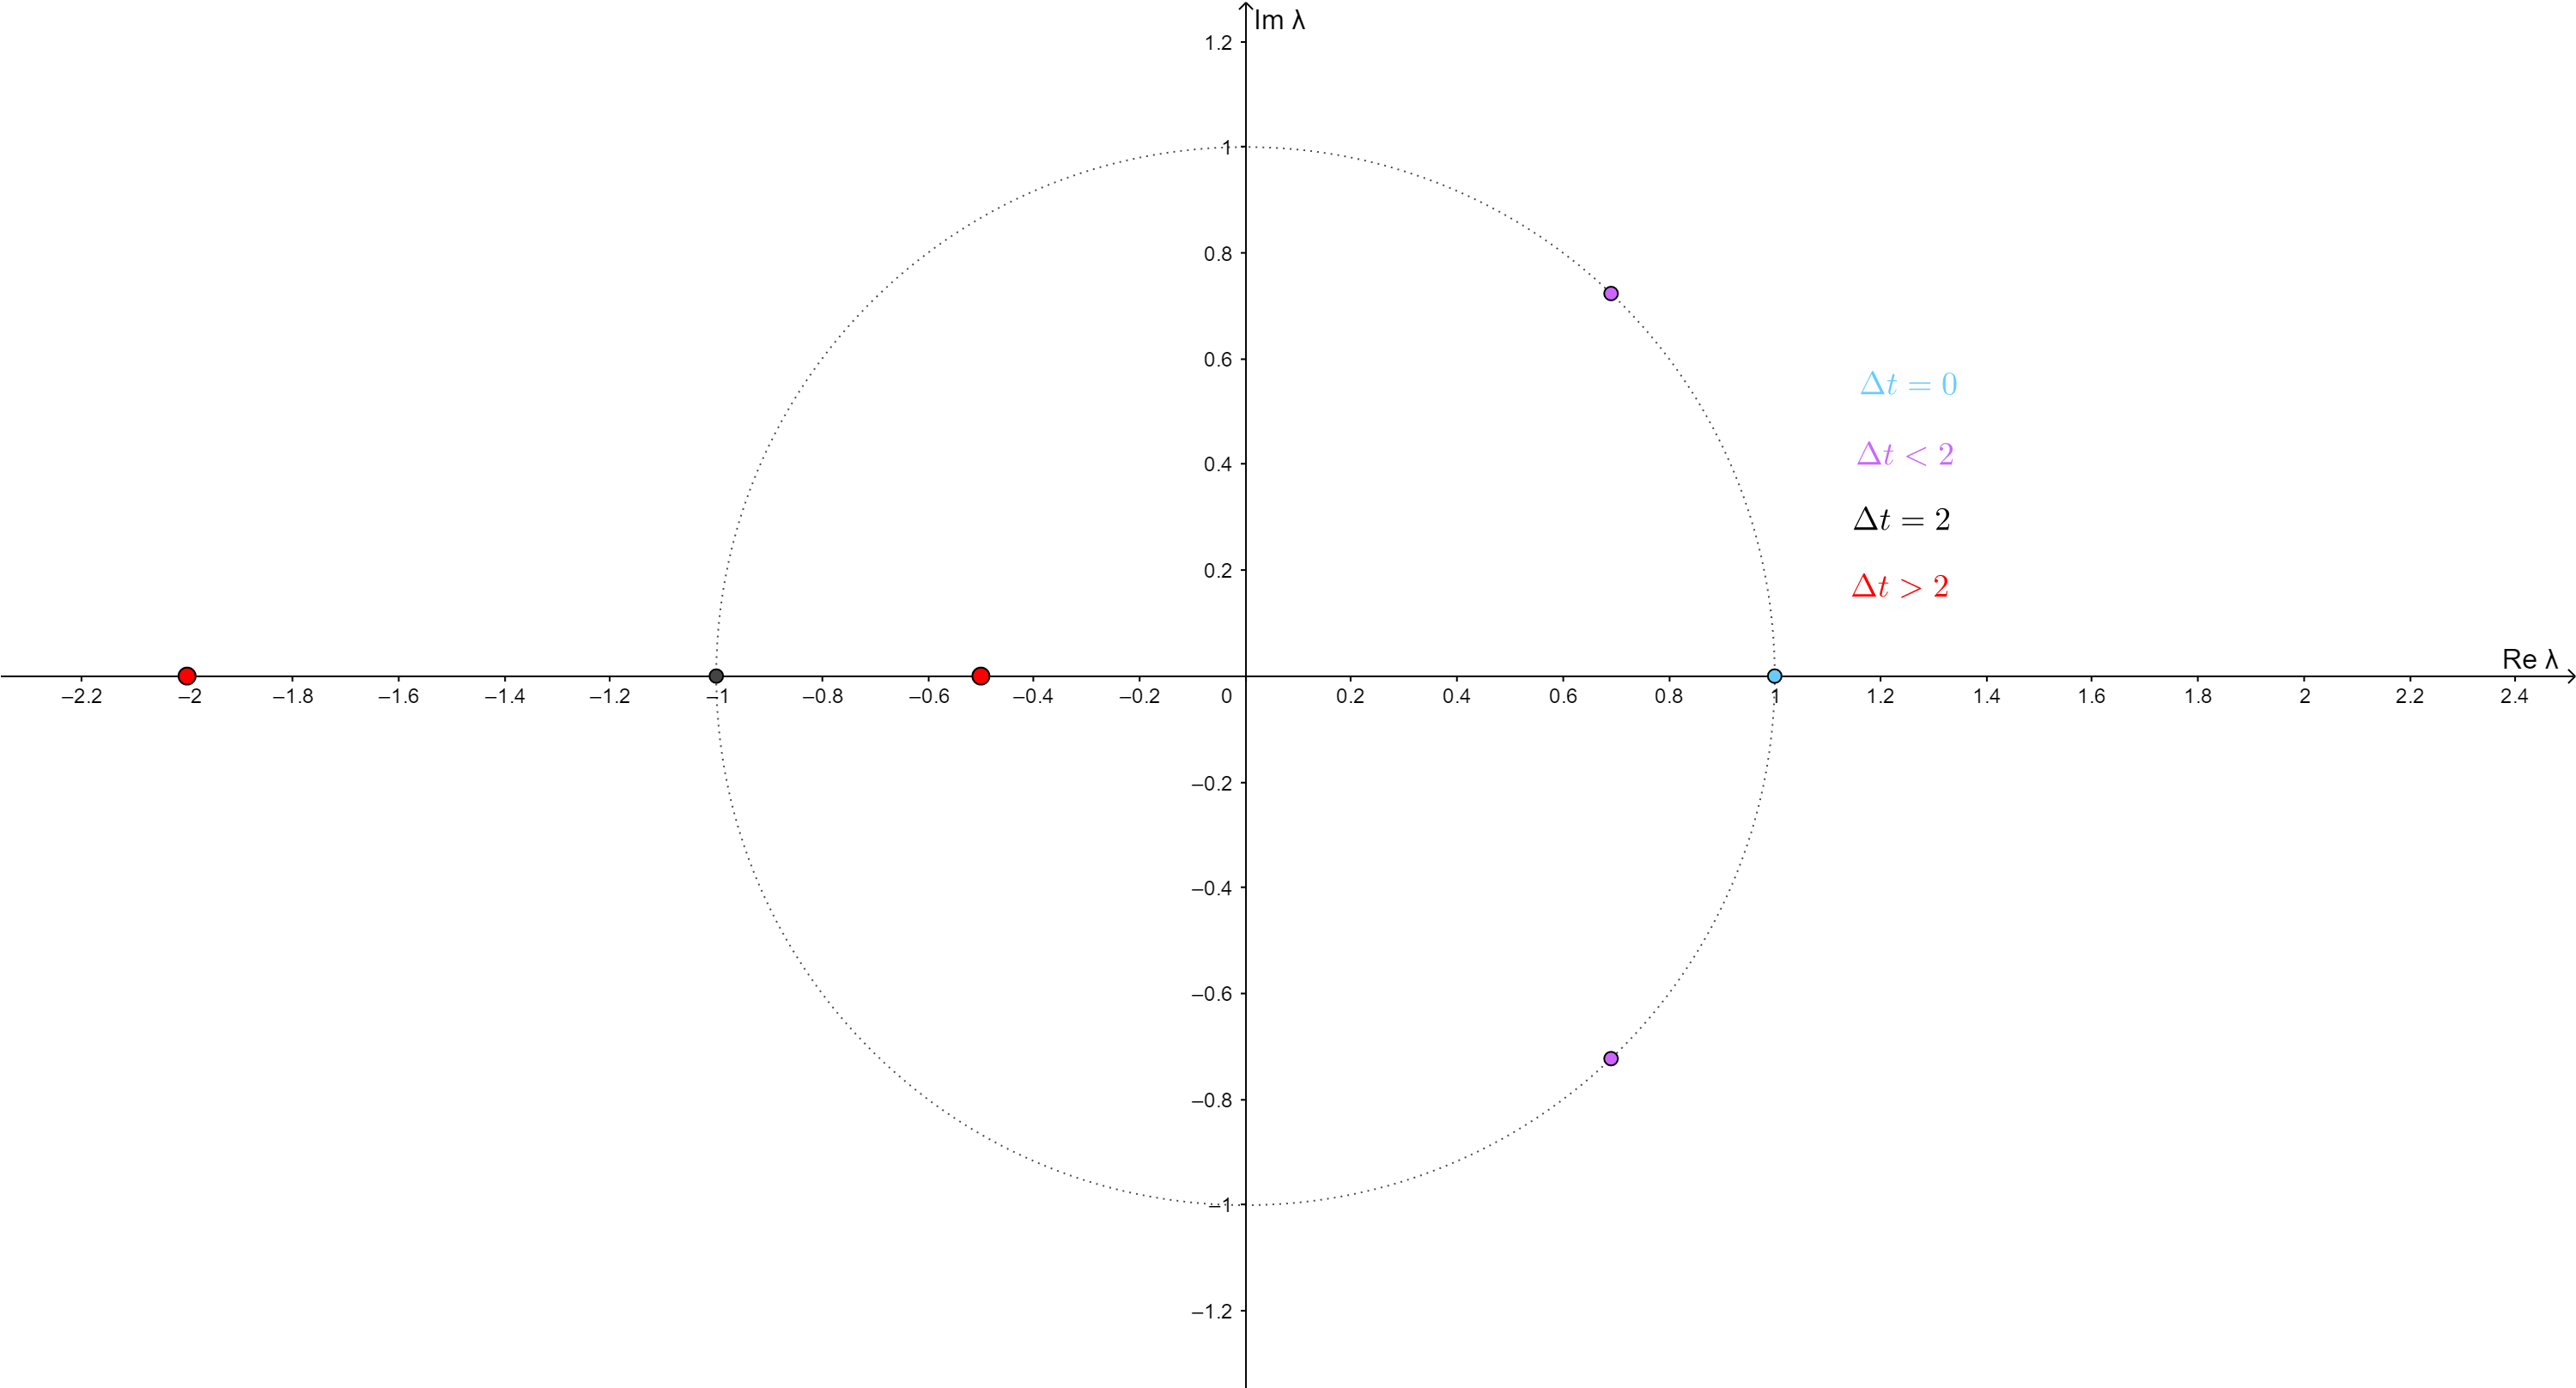
\includegraphics[scale=3.0]{Integrators/images/complexplane.png}
    \caption{Possible eigenvalues of the matrix $A$}
    \label{fig:complexplane}
\end{figure}
In the case where they are complex, their imaginary part is opposite and the real parts are equal.
After n steps:
\begin{equation}
    \begin{pmatrix}
      q' \\
      p'
    \end{pmatrix}
    = A^n
    \begin{pmatrix}
      q \\
      p
    \end{pmatrix}
\end{equation}
Check the behaviour for a large number of time steps ($n\xrightarrow{}\infty$):
\begin{itemize}
    \item if $A^n$ contains some infinite term, then the trajectory will diverge.
    \item if $A^n$ goes to 0, then the trajectory will converge (oscillate around the circular trajectory).
\end{itemize}
The eigenvalues of $A^n$ are equal to the eigenvalues of $A$ raised to the n-th power, therefore:
\begin{itemize}
    \item  $\lambda_1=\lambda_2=-1$: trajectory will oscillate\footnote{$\lambda_1=\lambda_2=1$ is the case when the timestep is equal to zero, therefore the system is not moving}. $$\Delta t = 2$$
    \item $\lambda_1> -1$, $\lambda_2< -1$ or $\lambda_2> -1$, $\lambda_1< -1$: matrix explodes, trajectory diverges. $$\Delta t > 2$$
    \item complex eigenvalues with unitary modulus: trajectory will oscillate.  $$\Delta t < 2$$
\end{itemize}
Threshold for stability of a numerical simulation:
\begin{equation}
    \Delta t < \frac{T}{\pi}
\end{equation}
This is the theoretical limit for the timestep, given the period. The criterion for the timestep is the same for Verlet and Velocity Verlet.
\subsection{Multiple springs}
Let us consider a situation where there are 3 particles with the same mass connected by springs with $k_1 >> k_2$. Let us estimate the maximum time step that should be used. The solution is to take the stiffest spring to impose the limit on the timestep, i.e., that gives the shortest timestep.
In general, this condition is given by the fastest degree of freedom, in other words, by the lightest possible atom with the stiffest spring. This is the way to find the upper bound for our timestep:
computing the period $2\pi \sqrt{\frac{m}{k}}$.
If energy is sufficiently conserved, this means that the timestep is small enough. It is difficult to predict a priori a good value of the timestep because there could be nonlinear potentials.


    \section{The Gran-Canonical ensemble}
Let's now consider a system for which the number of particles is allowed to fluctuate, as if the system were in contact with a larger system at the same temperature, with which it can exchange particles. In order to treat this case, we need to add to the phase space distribution function an extra index accounting for the number of particles N:
\begin{equation}
    \rho(\textbf{q},\textbf{p}) \rightarrow \rho_N(\textbf{q},\textbf{p}).
\end{equation}
A more general definition of Entropy may be written too:
\begin{equation}
        S = -k_B \sum_N \int \frac{d\Gamma_N}{h^{3N}}  \rho_N\ln{\rho_N},\label{S}
\end{equation}
  This corresponds to the most general integration over phase space of the expression $\rho_N\ln{\rho_N}$. $h^{3N}$ is a dimensional factor deriving from quantization of phase space. Being it a constant, we will neglect this factor from now on. Again, due to the maximum entropy principle, an expression for the density $\rho_N$ can be found maximizing entropy with the appropriate constraints:
\begin{itemize}
    \item $\sum_N \int d\Gamma_N  \rho_N = 1 \: \Rightarrow \: \text{normalization} $\\
    \item $\sum_N \int d\Gamma_N  \rho_N H_N = <E> \: \Rightarrow \: \text{mean energy conservation}\\$
    \item $\sum_N \int d\Gamma_N  \rho_N N = <N> \: \Rightarrow \: \text{mean n. of particles conservation}\\$
\end{itemize}
Hence, we're looking for $\rho_N^*$ such that the functional 
\begin{equation}
    \mathcal{F}[\rho_N] = -\sum_N\int d\Gamma_N \rho_N ( \ln{\rho_N} - \lambda + \beta H_N - \beta \mu N)
\end{equation}
is stationary. Imposing: 
\begin{align}
    \partial\mathcal{F}[\rho_N^*] &\equiv \mathcal{F}[\rho_N^*+\delta\rho_N] - \mathcal{F}[\rho_N^*]\\
    &\simeq -\sum_N\int d\Gamma_N \delta\rho_N(\ln{\rho_N^*}+1-\lambda+\beta H_N -\beta \mu N)=0
\end{align}
we get the following expression:
\begin{equation}
\label{eq:rho_micro}
    \rho_N^*=\frac{e^{-\beta(H_N-\mu N)}}{Z_{GC}}\:. 
\end{equation}
An \textit{ad hoc} extra factor $1/N!$ has to be introduced to obtain the correct additive Entropy (see Huang), so that the final result is:
\begin{equation}\label{incriminate} 
    \rho_N^*=\frac{e^{-\beta(H_N-\mu N)}}{N! Z_{GC}},\hspace{0.5 cm} \text{with} \: Z_{GC}= \sum_N\int d\Gamma_N \frac{e^{-\beta(H_N-\mu N)}}{N!}.
\end{equation}
The new Lagrange multiplier we have introduced, $\mu$, is called \textit{chemical potential}. We will later give an interpretation for it.\\

\textit{\textbf{Comment:} I believe Micheletti was imprecise here. In eq.\ref{incriminate} the factor $1/N!$ should be present in the expression for $Z$ but not in the one for $\rho$. Actually, if both expressions contained it, we would be multiplying $\rho$ for a $N!/N!=1$ factor and eq.\ref{S} would remain unchanged. The correct interpretation is the following: being atoms quantum mechanically indistinguishable, any permutation of the atoms indexes does not produce a new state of the system. Then the factor $1/N!$ accounts for the fact that an infinitesimal volume $dpdq$ in phase space corresponds to $dpdq/N!$ different micro-states only. In conclusion, when taking averages of functions $f(p,q)$ over the possible micro-states of the system, we should write integrals as:
\begin{equation}
    <f> = \sum_N \int \frac{d\Gamma_N}{N!h^{3N}}  \rho_N f(q,p).
\end{equation}
This explains why $1/N!$ is only present in the expression for $Z$. Also, computing entropy like this all factors $1/N!$ simplify apart from the one inside the logarithm, so that we obtain the correctly rescaled expression.
}\\

As an example, we can compute the Gran-Canonical partition function $Z_{GC}$ for an ideal gas:
\begin{equation}
    \begin{split}
    Z_{GC} &= \sum_N \frac{1}{N!}\int d\Gamma_N e^{-\beta(H_N-\mu N)}\\
    &=\sum_N \frac{e^{\beta \mu N}}{N!}\int d\Gamma_N e^{-\beta H_N}\\
    &=\sum_N \frac{e^{\beta \mu N}}{N!}V^N\biggl( \frac{2\pi m}{\beta}\biggr)^{3N/2}\\
    &=\sum_N \frac{x^N}{N!}=e^x, \hspace{0.5 cm} \text{with} \:x=e^{\beta \mu}V \biggl(\frac{2\pi m}{\beta}\biggr)^{3/2}.
    \end{split}
\end{equation}
We have used the expression \ref{eq:zcannone} for the Canonical partition function computed in the previous section. We call the factor $z=e^{\beta \mu}$ \textit{fugacity}. The mean number of particles $<N>$ can be computed too. Being $Z_{GC}$ a cumulant generating function, 
\begin{equation}
    <N>=\frac{\partial ln Z_{GC}}{\partial (\beta \mu)}
    =e^{\beta \mu}V \biggl(\frac{2\pi     m}{\beta}\biggr)^{3/2}. \label{eq.N}
\end{equation}
Consequently:
\begin{equation}
   \begin{split}
    & e^{-\beta \mu}=\frac{V}{<N>}\biggl(\frac{2\pi m}{\beta}\biggr)^{3/2} \\
    & \mu=-K_B T ln \biggl[\frac{V}{<N>}\biggl(\frac{2\pi m}{\beta}\biggr)^{3/2} \biggr].
    \end{split}
\end{equation}
The equation we have obtained for $\mu$ tells us something important about its physical interpretation. Recalling the equation for the \textit{free energy} for a canonical ensemble in the case of an ideal gas,
\begin{equation}
    \begin{split}
    F_{CAN}&=-k_B T \ln{Z_{CAN}}\\
    &=-k_B T ln\biggl[ \frac{V^N}{N!}\left(\frac{2\pi m}{\beta} \right)^{3N/2}\biggr]\\
    &=-k_B T \biggl[N\ln{V}-ln(N!)+\frac{3N}{2}\ln{\left(\frac{2\pi m}{\beta} \right)}\biggr]\\
    &\simeq -k_B T \biggl[N\ln{V}-(NlnN-N)+\frac{3N}{2}\ln{\left(\frac{2\pi m}{\beta} \right)}\biggr],\\
    \end{split}
\end{equation}
where we have used Stirling's approximation, we have that:
\begin{equation}
   \frac{\partial F_{CAN}}{\partial N}=-K_B T ln \biggl[\frac{V}{N}\biggl(\frac{2\pi m}{\beta}\biggr)^{3/2} \biggr]=\mu.
\end{equation}
In conclusion, $\mu$ corresponds to the difference in \textit{free energy} due to variations of the number of particles the system is composed of.

\subsection{Equilibrium condition for chemical reactions}
The \textit{chemical potential} $\mu$ turns out to be very useful in some chemistry problems. Let's consider a generic chemical reaction involving n reactants and m products:
\begin{equation}
    \nu_1 x_1 + ... + \nu_n x_n \rightleftharpoons \nu_{n+1} x_{n+1} + ... + \nu_{n+m} x_{n+m}
\end{equation}
Clearly, when elements react, the number of molecules $N_i$ of element i varies: $N_i \rightarrow N_i+\delta N_i$. This makes the system we're studying a Gran-Canonical one. On the other hand, starting from equilibrium, the ratio $\delta N_i/\nu_i$ between the variation of the number of molecules of element i and its stoichiometric coefficient must be constant and equal for all i's. Also, if the system keeps at equilibrium the \textit{free energy} F must be minimal. Then:
\begin{equation}
    \begin{split}
    \partial F &= F(N_1+\delta N_1,...,N_{n+m}+\delta N_{n+m})-F(N_1,...,N_{n+m})\\
    &=\frac{\partial F}{\partial N_1}\delta N_1+...+\frac{\partial F}{\partial N_{n+m}}\delta N_{n+m}\\
    &=\mu_1 \delta N_1+...+\mu_{n+m} \delta N_{n+m}=0.
    \end{split}
\end{equation}
Knowing $\delta N_i/\nu_i= const=\delta N$, with $\delta N$ arbitrary, we get to the equilibrium condition:
\begin{equation}
    \sum_i \mu_i \nu_i=0.
\end{equation}
Notice that, for convention, stoichiometric coefficients $\nu_i$ are positive for reactants and negative for products. This same condition may be written in terms of the fugacity $z$ as:
\begin{equation}
    e^{\beta\sum_i \mu_i \nu_i}=\prod_i (z_i)^{\nu_i}=1.\label{eq.fugacity}
\end{equation}
From eq.\ref{eq.N}:
\begin{equation}
    z=\bigl[ v \bigl( \frac{2\pi m}{\beta}\bigr)^{3/2}\bigr]^{-1}, 
\end{equation}
where $v=\frac{V}{N}$ is the concentration of the $i_{th}$ element. Then eq.\ref{eq.fugacity} tells us:
\begin{equation}
    \prod_i v_i^{\nu_i}\sim\prod_i (m^{\nu_i})^{-3/2}.  
\end{equation}
This is known as the law of mass action, stating that the the quantity $\prod_i v_i^{\nu_i}$ is a constant for reactions at equilibrium, namely the \textit{equilibrium constant}.  
%\chapter{Exercises}
  %  \section{Verlet Exercise}
 %   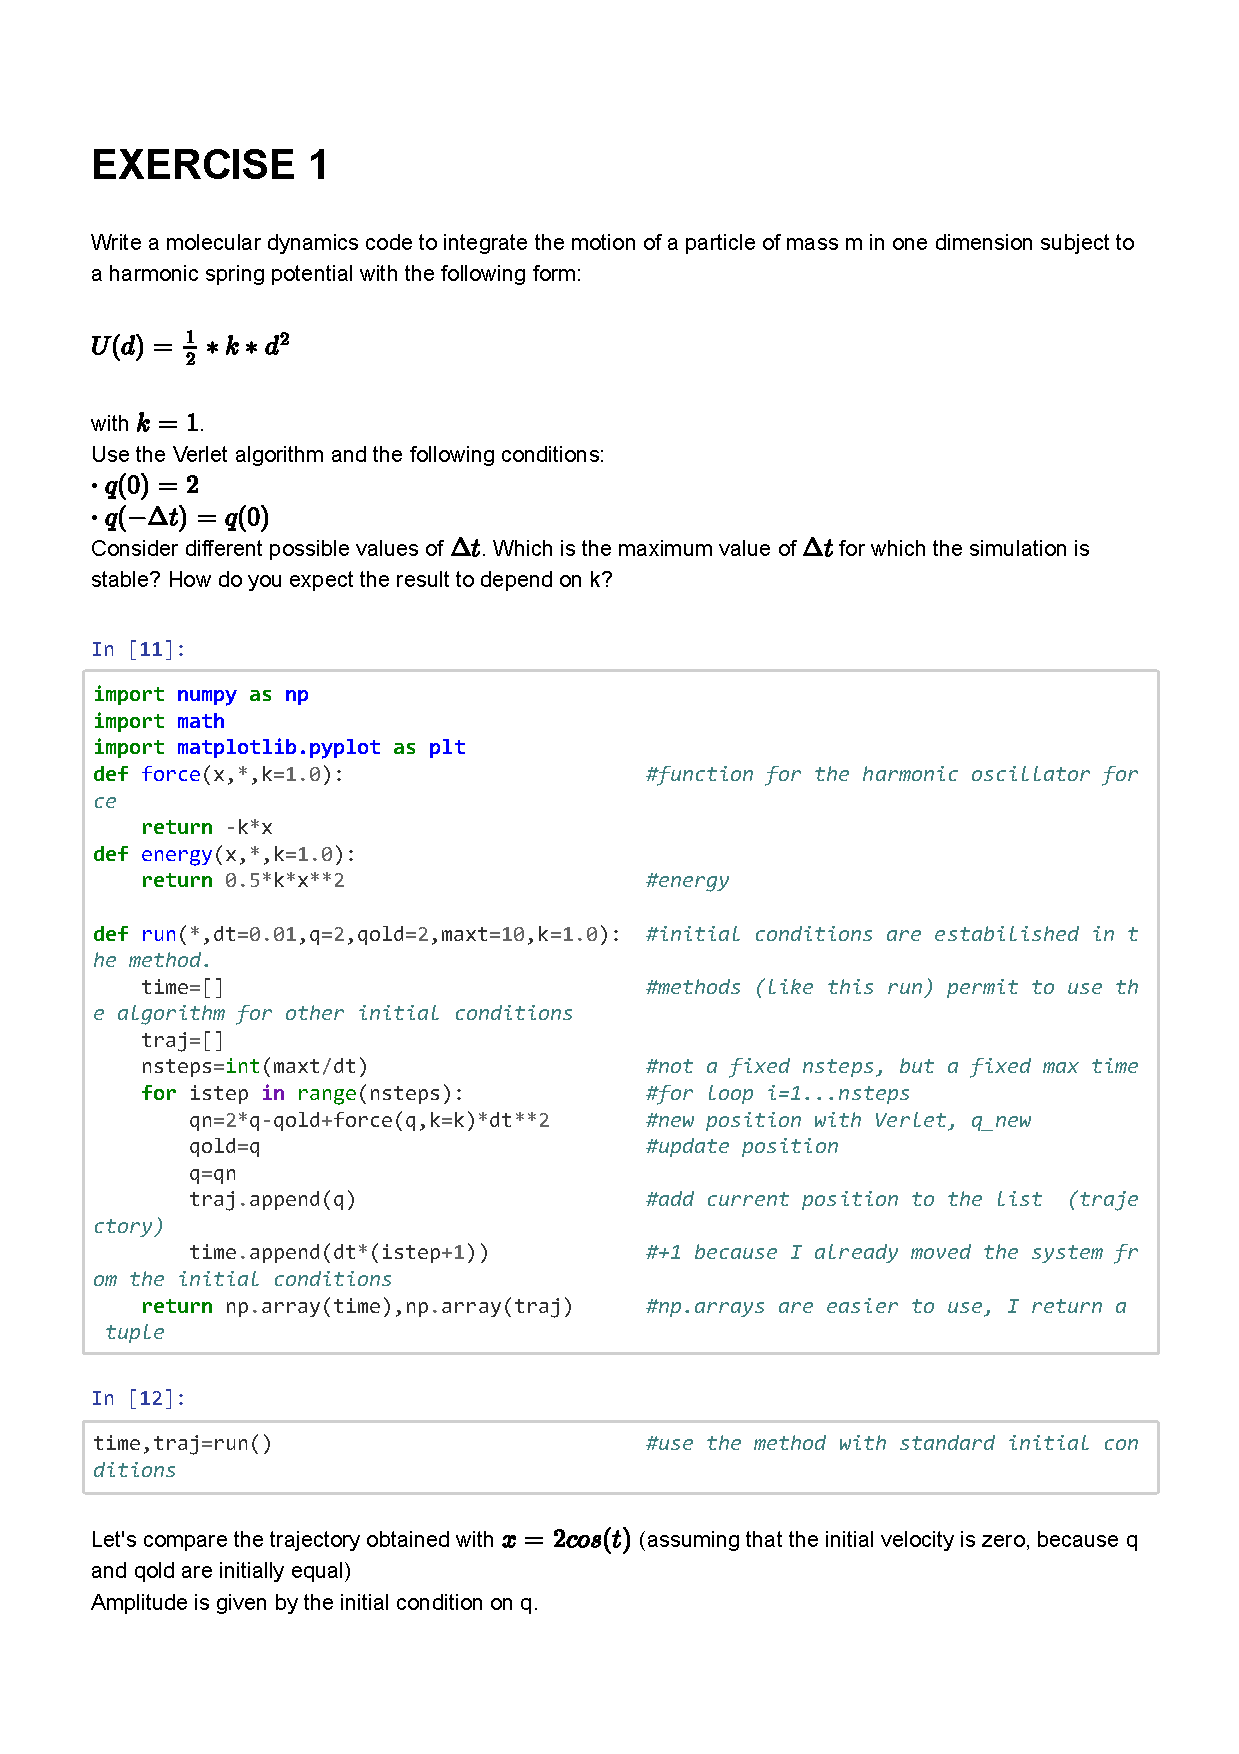
\includepdf[pages=-]{Integrators/ex1.pdf}
%    \section{MC exercise}
%    We will propose a solution for the MC exercise. The code has been commented widely to make it more readable.
%    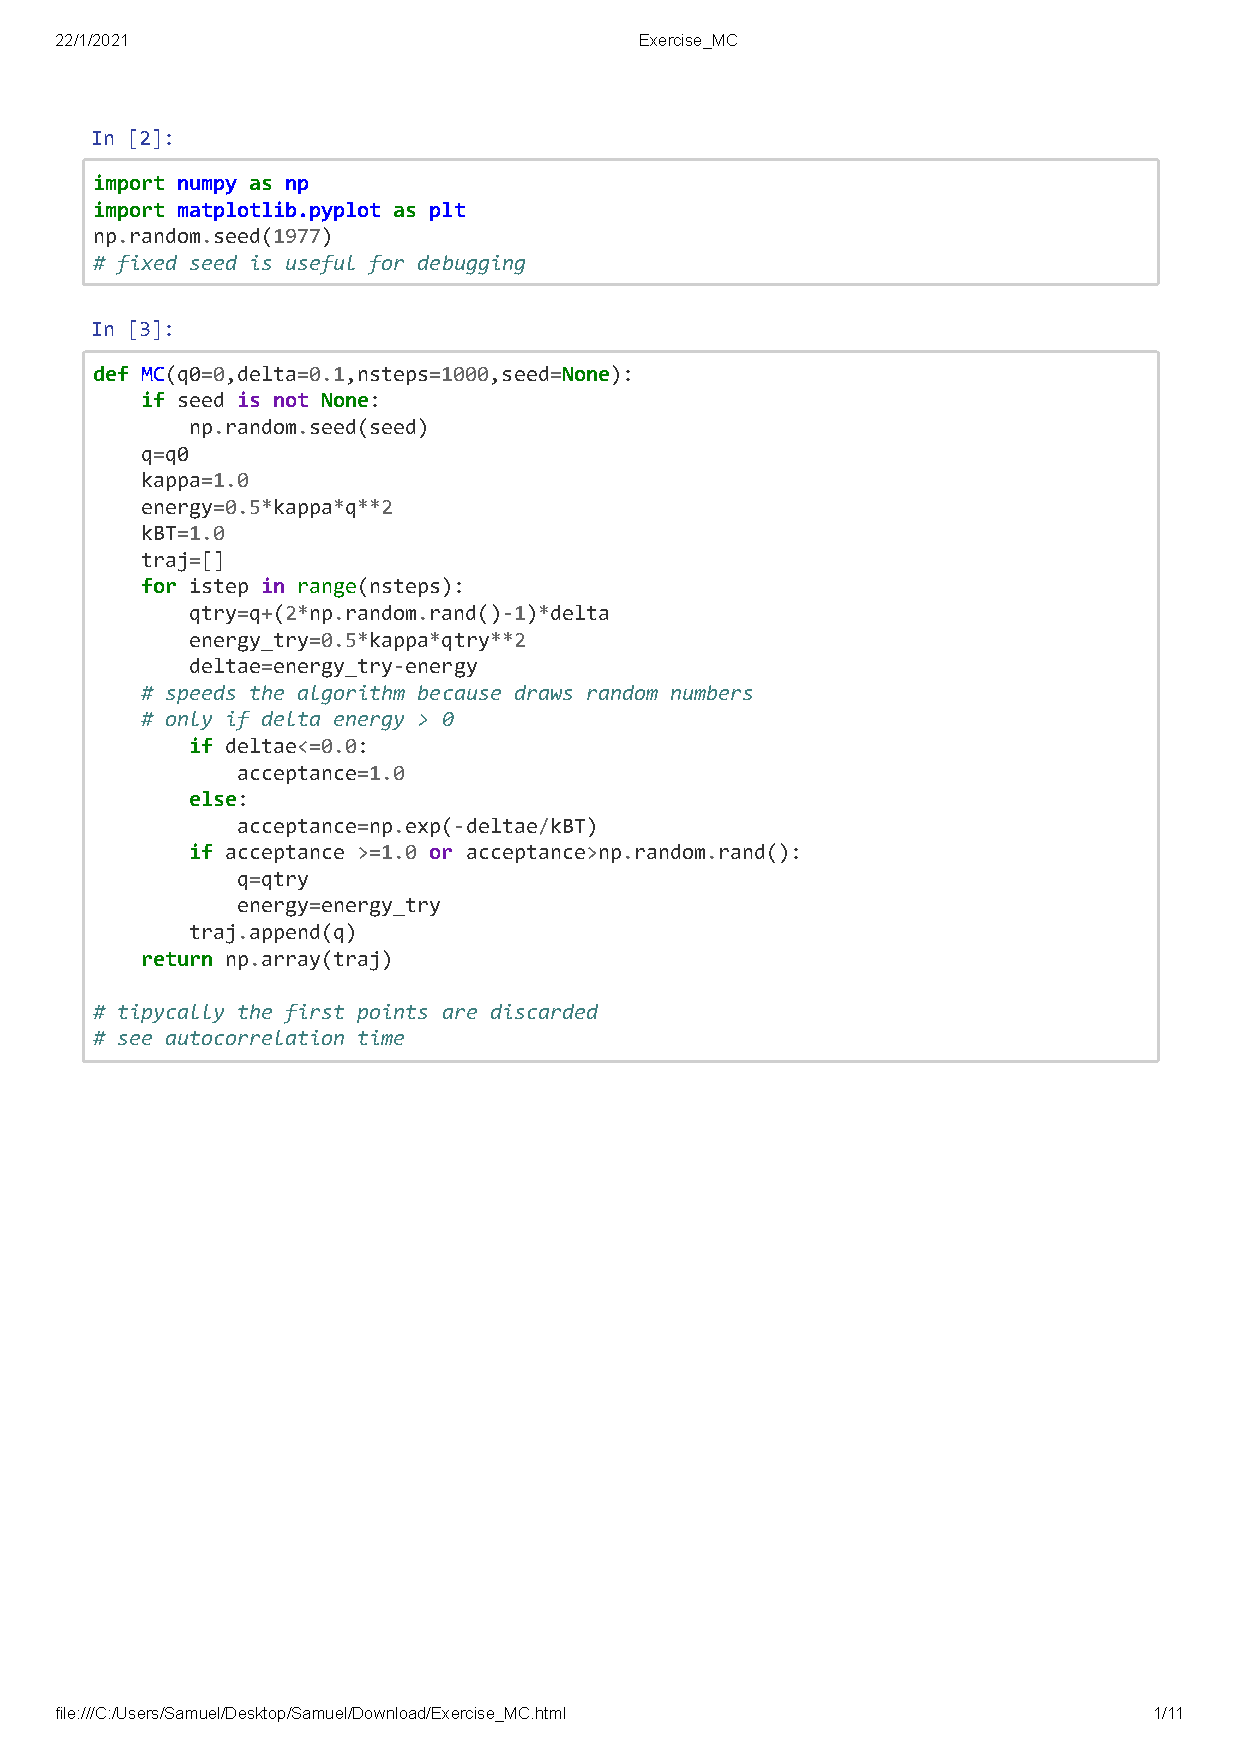
\includepdf[pages=-]{Exercise_MC.pdf}
%From the last result we can make an important observation. The result for the mean distance is $4.4$ and not $4$ as one would have naively expected. This comes out because in a three dimensional system, such as the one of the two particles considered in the problem, the number of available states scales like $r^2$, where $r$ is the distance between the two particles. Therefore in computing the average distance there is an additional entropic term, that shifts away a little the average distance from the minimum of the energy. If one evaluates analytically this quantity, this factor comes out naturally using the canonical distribution and performing a change of variables in the integral from cartesian to spherical coordinates.
%    \section{SDE Exercise}
%    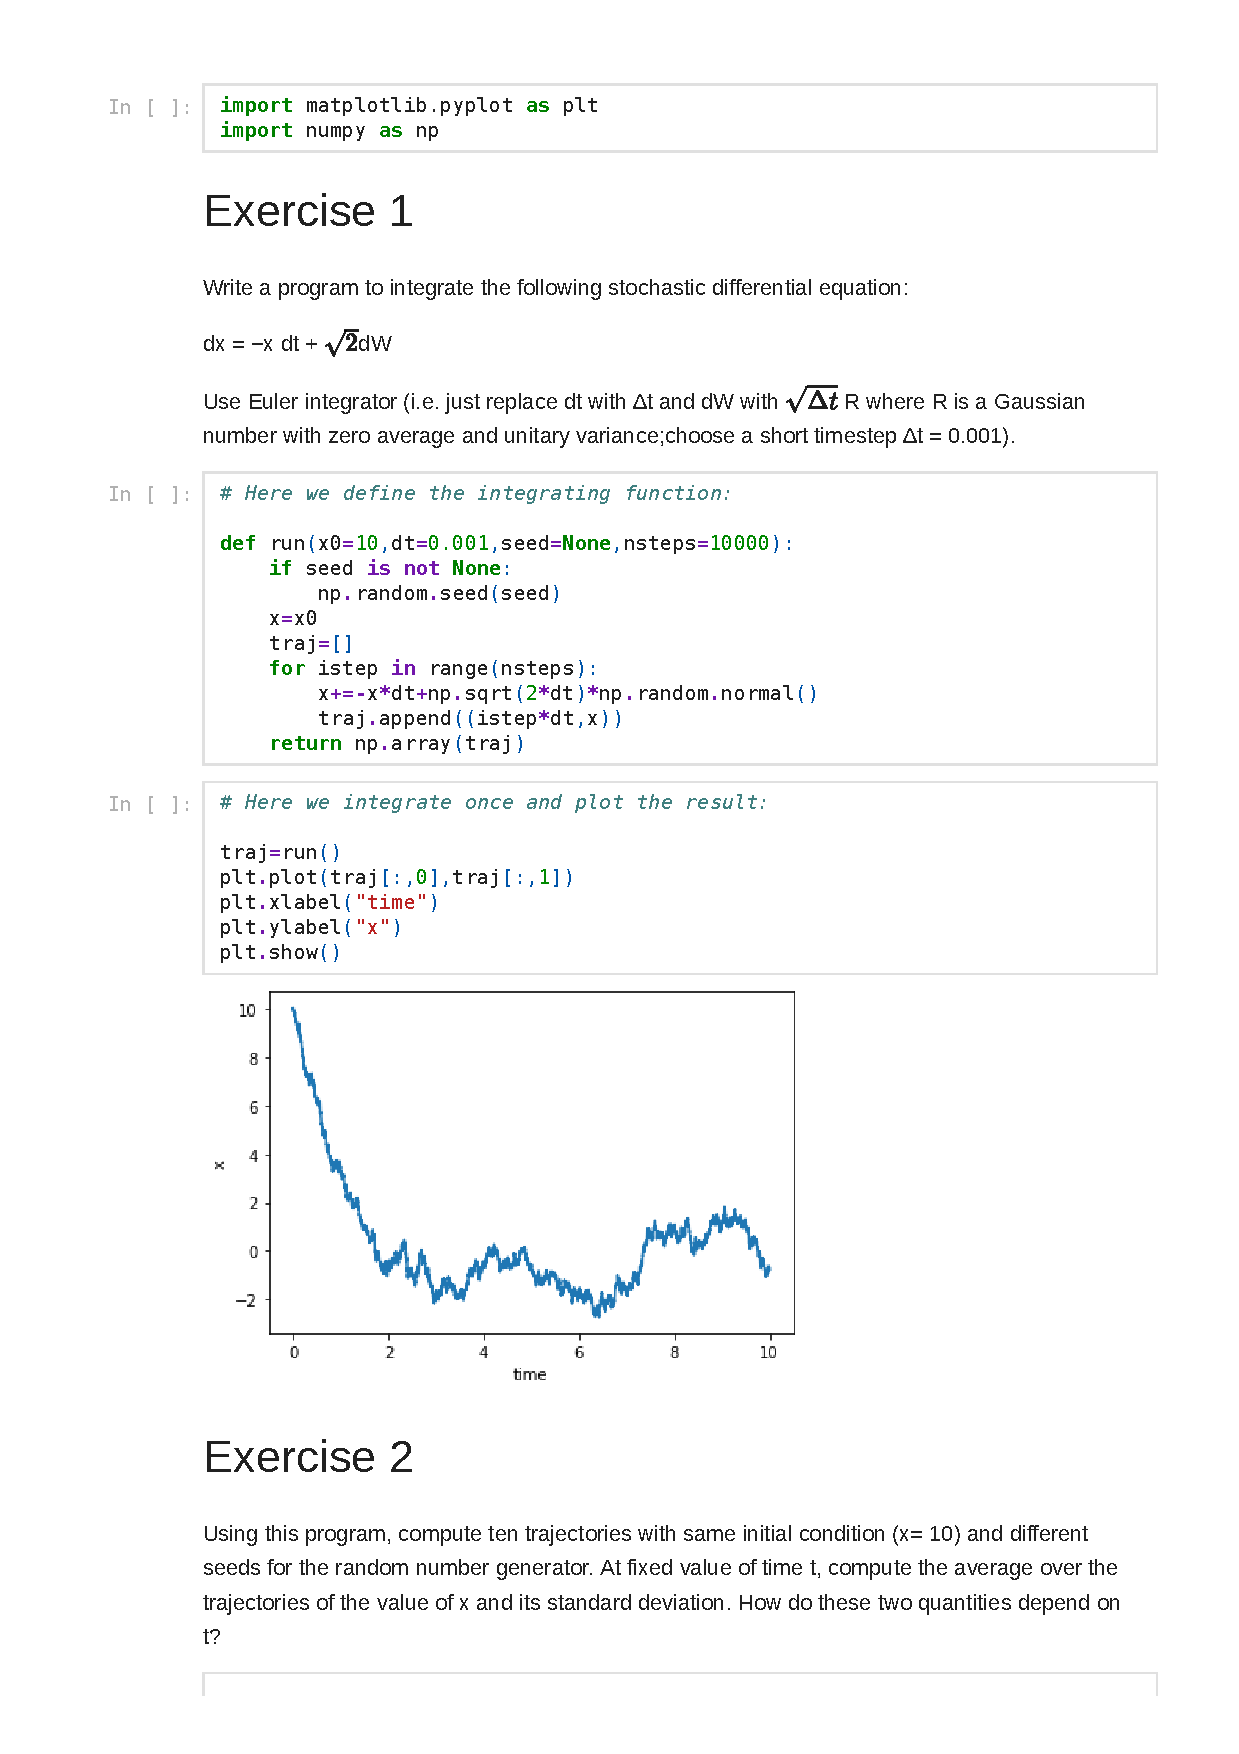
\includepdf[pages=-]{SDE/bussi_es.pdf}
%    \section{Thermostats Exercise}
%    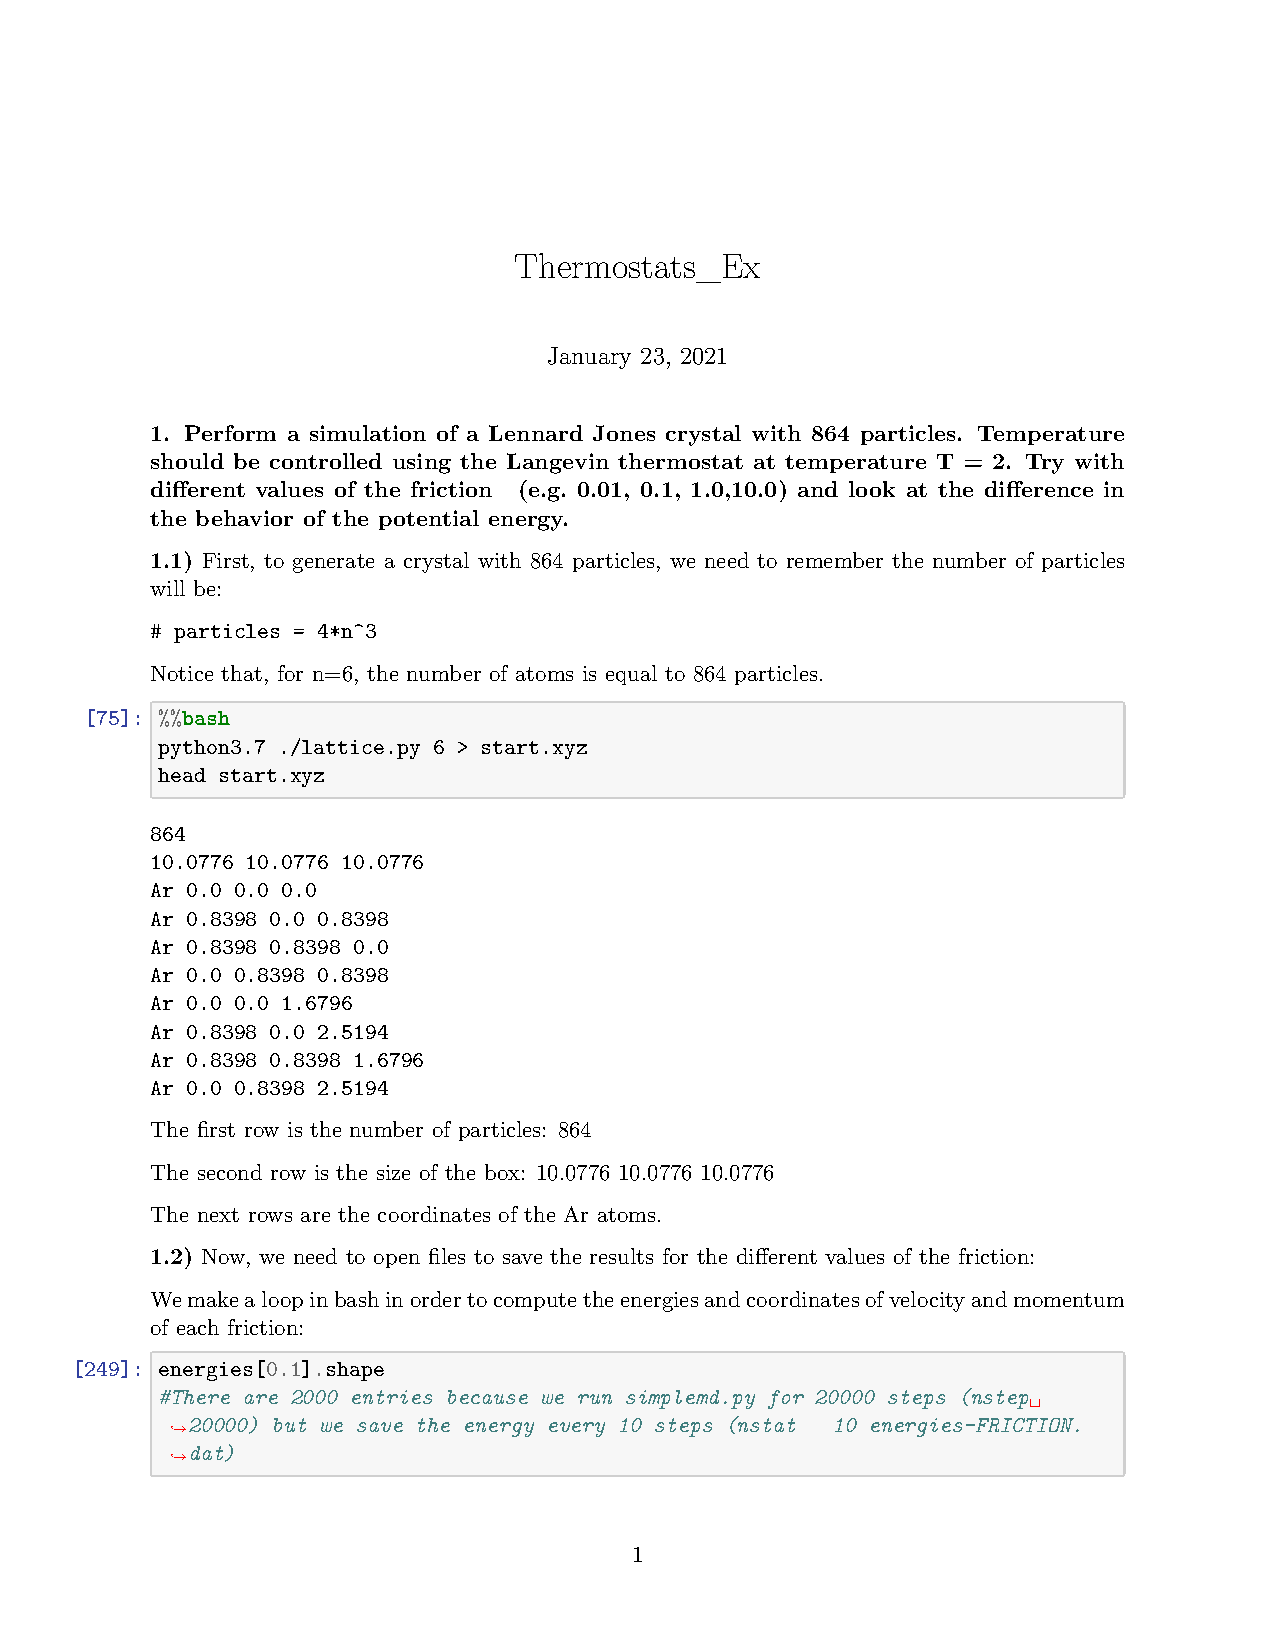
\includepdf[pages=-]{Thermostats_Ex.pdf}
\bibliographystyle{unsrt}
\bibliography{bibliography}
\end{document}
